


% Header, overrides base

    % Make sure that the sphinx doc style knows who it inherits from.
    \def\sphinxdocclass{article}

    % Declare the document class
    \documentclass[letterpaper,10pt,english]{/Users/edwsurewin/anaconda/lib/python2.7/site-packages/sphinx/texinputs/sphinxhowto}

    % Imports
    \usepackage[utf8]{inputenc}
    \DeclareUnicodeCharacter{00A0}{\\nobreakspace}
    \usepackage[T1]{fontenc}
    \usepackage{babel}
    \usepackage{times}
    \usepackage{import}
    \usepackage[Bjarne]{/Users/edwsurewin/anaconda/lib/python2.7/site-packages/sphinx/texinputs/fncychap}
    \usepackage{longtable}
    \usepackage{/Users/edwsurewin/anaconda/lib/python2.7/site-packages/sphinx/texinputs/sphinx}
    \usepackage{multirow}

    \usepackage{amsmath}
    \usepackage{amssymb}
    \usepackage{ucs}
    \usepackage{enumerate}

    % Used to make the Input/Output rules follow around the contents.
    \usepackage{needspace}

    % Pygments requirements
    \usepackage{fancyvrb}
    \usepackage{color}
    % ansi colors additions
    \definecolor{darkgreen}{rgb}{.12,.54,.11}
    \definecolor{lightgray}{gray}{.95}
    \definecolor{brown}{rgb}{0.54,0.27,0.07}
    \definecolor{purple}{rgb}{0.5,0.0,0.5}
    \definecolor{darkgray}{gray}{0.25}
    \definecolor{lightred}{rgb}{1.0,0.39,0.28}
    \definecolor{lightgreen}{rgb}{0.48,0.99,0.0}
    \definecolor{lightblue}{rgb}{0.53,0.81,0.92}
    \definecolor{lightpurple}{rgb}{0.87,0.63,0.87}
    \definecolor{lightcyan}{rgb}{0.5,1.0,0.83}

    % Needed to box output/input
    \usepackage{tikz}
        \usetikzlibrary{calc,arrows,shadows}
    \usepackage[framemethod=tikz]{mdframed}

    \usepackage{alltt}

    % Used to load and display graphics
    \usepackage{graphicx}
    \graphicspath{ {figs/} }
    \usepackage[Export]{adjustbox} % To resize

    % used so that images for notebooks which have spaces in the name can still be included
    \usepackage{grffile}


    % For formatting output while also word wrapping.
    \usepackage{listings}
    \lstset{breaklines=true}
    \lstset{basicstyle=\small\ttfamily}
    \def\smaller{\fontsize{9.5pt}{9.5pt}\selectfont}

    %Pygments definitions
    
\makeatletter
\def\PY@reset{\let\PY@it=\relax \let\PY@bf=\relax%
    \let\PY@ul=\relax \let\PY@tc=\relax%
    \let\PY@bc=\relax \let\PY@ff=\relax}
\def\PY@tok#1{\csname PY@tok@#1\endcsname}
\def\PY@toks#1+{\ifx\relax#1\empty\else%
    \PY@tok{#1}\expandafter\PY@toks\fi}
\def\PY@do#1{\PY@bc{\PY@tc{\PY@ul{%
    \PY@it{\PY@bf{\PY@ff{#1}}}}}}}
\def\PY#1#2{\PY@reset\PY@toks#1+\relax+\PY@do{#2}}

\expandafter\def\csname PY@tok@gd\endcsname{\def\PY@tc##1{\textcolor[rgb]{0.63,0.00,0.00}{##1}}}
\expandafter\def\csname PY@tok@gu\endcsname{\let\PY@bf=\textbf\def\PY@tc##1{\textcolor[rgb]{0.50,0.00,0.50}{##1}}}
\expandafter\def\csname PY@tok@gt\endcsname{\def\PY@tc##1{\textcolor[rgb]{0.00,0.27,0.87}{##1}}}
\expandafter\def\csname PY@tok@gs\endcsname{\let\PY@bf=\textbf}
\expandafter\def\csname PY@tok@gr\endcsname{\def\PY@tc##1{\textcolor[rgb]{1.00,0.00,0.00}{##1}}}
\expandafter\def\csname PY@tok@cm\endcsname{\let\PY@it=\textit\def\PY@tc##1{\textcolor[rgb]{0.25,0.50,0.50}{##1}}}
\expandafter\def\csname PY@tok@vg\endcsname{\def\PY@tc##1{\textcolor[rgb]{0.10,0.09,0.49}{##1}}}
\expandafter\def\csname PY@tok@m\endcsname{\def\PY@tc##1{\textcolor[rgb]{0.40,0.40,0.40}{##1}}}
\expandafter\def\csname PY@tok@mh\endcsname{\def\PY@tc##1{\textcolor[rgb]{0.40,0.40,0.40}{##1}}}
\expandafter\def\csname PY@tok@go\endcsname{\def\PY@tc##1{\textcolor[rgb]{0.53,0.53,0.53}{##1}}}
\expandafter\def\csname PY@tok@ge\endcsname{\let\PY@it=\textit}
\expandafter\def\csname PY@tok@vc\endcsname{\def\PY@tc##1{\textcolor[rgb]{0.10,0.09,0.49}{##1}}}
\expandafter\def\csname PY@tok@il\endcsname{\def\PY@tc##1{\textcolor[rgb]{0.40,0.40,0.40}{##1}}}
\expandafter\def\csname PY@tok@cs\endcsname{\let\PY@it=\textit\def\PY@tc##1{\textcolor[rgb]{0.25,0.50,0.50}{##1}}}
\expandafter\def\csname PY@tok@cp\endcsname{\def\PY@tc##1{\textcolor[rgb]{0.74,0.48,0.00}{##1}}}
\expandafter\def\csname PY@tok@gi\endcsname{\def\PY@tc##1{\textcolor[rgb]{0.00,0.63,0.00}{##1}}}
\expandafter\def\csname PY@tok@gh\endcsname{\let\PY@bf=\textbf\def\PY@tc##1{\textcolor[rgb]{0.00,0.00,0.50}{##1}}}
\expandafter\def\csname PY@tok@ni\endcsname{\let\PY@bf=\textbf\def\PY@tc##1{\textcolor[rgb]{0.60,0.60,0.60}{##1}}}
\expandafter\def\csname PY@tok@nl\endcsname{\def\PY@tc##1{\textcolor[rgb]{0.63,0.63,0.00}{##1}}}
\expandafter\def\csname PY@tok@nn\endcsname{\let\PY@bf=\textbf\def\PY@tc##1{\textcolor[rgb]{0.00,0.00,1.00}{##1}}}
\expandafter\def\csname PY@tok@no\endcsname{\def\PY@tc##1{\textcolor[rgb]{0.53,0.00,0.00}{##1}}}
\expandafter\def\csname PY@tok@na\endcsname{\def\PY@tc##1{\textcolor[rgb]{0.49,0.56,0.16}{##1}}}
\expandafter\def\csname PY@tok@nb\endcsname{\def\PY@tc##1{\textcolor[rgb]{0.00,0.50,0.00}{##1}}}
\expandafter\def\csname PY@tok@nc\endcsname{\let\PY@bf=\textbf\def\PY@tc##1{\textcolor[rgb]{0.00,0.00,1.00}{##1}}}
\expandafter\def\csname PY@tok@nd\endcsname{\def\PY@tc##1{\textcolor[rgb]{0.67,0.13,1.00}{##1}}}
\expandafter\def\csname PY@tok@ne\endcsname{\let\PY@bf=\textbf\def\PY@tc##1{\textcolor[rgb]{0.82,0.25,0.23}{##1}}}
\expandafter\def\csname PY@tok@nf\endcsname{\def\PY@tc##1{\textcolor[rgb]{0.00,0.00,1.00}{##1}}}
\expandafter\def\csname PY@tok@si\endcsname{\let\PY@bf=\textbf\def\PY@tc##1{\textcolor[rgb]{0.73,0.40,0.53}{##1}}}
\expandafter\def\csname PY@tok@s2\endcsname{\def\PY@tc##1{\textcolor[rgb]{0.73,0.13,0.13}{##1}}}
\expandafter\def\csname PY@tok@vi\endcsname{\def\PY@tc##1{\textcolor[rgb]{0.10,0.09,0.49}{##1}}}
\expandafter\def\csname PY@tok@nt\endcsname{\let\PY@bf=\textbf\def\PY@tc##1{\textcolor[rgb]{0.00,0.50,0.00}{##1}}}
\expandafter\def\csname PY@tok@nv\endcsname{\def\PY@tc##1{\textcolor[rgb]{0.10,0.09,0.49}{##1}}}
\expandafter\def\csname PY@tok@s1\endcsname{\def\PY@tc##1{\textcolor[rgb]{0.73,0.13,0.13}{##1}}}
\expandafter\def\csname PY@tok@sh\endcsname{\def\PY@tc##1{\textcolor[rgb]{0.73,0.13,0.13}{##1}}}
\expandafter\def\csname PY@tok@sc\endcsname{\def\PY@tc##1{\textcolor[rgb]{0.73,0.13,0.13}{##1}}}
\expandafter\def\csname PY@tok@sx\endcsname{\def\PY@tc##1{\textcolor[rgb]{0.00,0.50,0.00}{##1}}}
\expandafter\def\csname PY@tok@bp\endcsname{\def\PY@tc##1{\textcolor[rgb]{0.00,0.50,0.00}{##1}}}
\expandafter\def\csname PY@tok@c1\endcsname{\let\PY@it=\textit\def\PY@tc##1{\textcolor[rgb]{0.25,0.50,0.50}{##1}}}
\expandafter\def\csname PY@tok@kc\endcsname{\let\PY@bf=\textbf\def\PY@tc##1{\textcolor[rgb]{0.00,0.50,0.00}{##1}}}
\expandafter\def\csname PY@tok@c\endcsname{\let\PY@it=\textit\def\PY@tc##1{\textcolor[rgb]{0.25,0.50,0.50}{##1}}}
\expandafter\def\csname PY@tok@mf\endcsname{\def\PY@tc##1{\textcolor[rgb]{0.40,0.40,0.40}{##1}}}
\expandafter\def\csname PY@tok@err\endcsname{\def\PY@bc##1{\setlength{\fboxsep}{0pt}\fcolorbox[rgb]{1.00,0.00,0.00}{1,1,1}{\strut ##1}}}
\expandafter\def\csname PY@tok@kd\endcsname{\let\PY@bf=\textbf\def\PY@tc##1{\textcolor[rgb]{0.00,0.50,0.00}{##1}}}
\expandafter\def\csname PY@tok@ss\endcsname{\def\PY@tc##1{\textcolor[rgb]{0.10,0.09,0.49}{##1}}}
\expandafter\def\csname PY@tok@sr\endcsname{\def\PY@tc##1{\textcolor[rgb]{0.73,0.40,0.53}{##1}}}
\expandafter\def\csname PY@tok@mo\endcsname{\def\PY@tc##1{\textcolor[rgb]{0.40,0.40,0.40}{##1}}}
\expandafter\def\csname PY@tok@kn\endcsname{\let\PY@bf=\textbf\def\PY@tc##1{\textcolor[rgb]{0.00,0.50,0.00}{##1}}}
\expandafter\def\csname PY@tok@mi\endcsname{\def\PY@tc##1{\textcolor[rgb]{0.40,0.40,0.40}{##1}}}
\expandafter\def\csname PY@tok@gp\endcsname{\let\PY@bf=\textbf\def\PY@tc##1{\textcolor[rgb]{0.00,0.00,0.50}{##1}}}
\expandafter\def\csname PY@tok@o\endcsname{\def\PY@tc##1{\textcolor[rgb]{0.40,0.40,0.40}{##1}}}
\expandafter\def\csname PY@tok@kr\endcsname{\let\PY@bf=\textbf\def\PY@tc##1{\textcolor[rgb]{0.00,0.50,0.00}{##1}}}
\expandafter\def\csname PY@tok@s\endcsname{\def\PY@tc##1{\textcolor[rgb]{0.73,0.13,0.13}{##1}}}
\expandafter\def\csname PY@tok@kp\endcsname{\def\PY@tc##1{\textcolor[rgb]{0.00,0.50,0.00}{##1}}}
\expandafter\def\csname PY@tok@w\endcsname{\def\PY@tc##1{\textcolor[rgb]{0.73,0.73,0.73}{##1}}}
\expandafter\def\csname PY@tok@kt\endcsname{\def\PY@tc##1{\textcolor[rgb]{0.69,0.00,0.25}{##1}}}
\expandafter\def\csname PY@tok@ow\endcsname{\let\PY@bf=\textbf\def\PY@tc##1{\textcolor[rgb]{0.67,0.13,1.00}{##1}}}
\expandafter\def\csname PY@tok@sb\endcsname{\def\PY@tc##1{\textcolor[rgb]{0.73,0.13,0.13}{##1}}}
\expandafter\def\csname PY@tok@k\endcsname{\let\PY@bf=\textbf\def\PY@tc##1{\textcolor[rgb]{0.00,0.50,0.00}{##1}}}
\expandafter\def\csname PY@tok@se\endcsname{\let\PY@bf=\textbf\def\PY@tc##1{\textcolor[rgb]{0.73,0.40,0.13}{##1}}}
\expandafter\def\csname PY@tok@sd\endcsname{\let\PY@it=\textit\def\PY@tc##1{\textcolor[rgb]{0.73,0.13,0.13}{##1}}}

\def\PYZbs{\char`\\}
\def\PYZus{\char`\_}
\def\PYZob{\char`\{}
\def\PYZcb{\char`\}}
\def\PYZca{\char`\^}
\def\PYZam{\char`\&}
\def\PYZlt{\char`\<}
\def\PYZgt{\char`\>}
\def\PYZsh{\char`\#}
\def\PYZpc{\char`\%}
\def\PYZdl{\char`\$}
\def\PYZhy{\char`\-}
\def\PYZsq{\char`\'}
\def\PYZdq{\char`\"}
\def\PYZti{\char`\~}
% for compatibility with earlier versions
\def\PYZat{@}
\def\PYZlb{[}
\def\PYZrb{]}
\makeatother


    %Set pygments styles if needed...
    
        \definecolor{nbframe-border}{rgb}{0.867,0.867,0.867}
        \definecolor{nbframe-bg}{rgb}{0.969,0.969,0.969}
        \definecolor{nbframe-in-prompt}{rgb}{0.0,0.0,0.502}
        \definecolor{nbframe-out-prompt}{rgb}{0.545,0.0,0.0}

        \newenvironment{ColorVerbatim}
        {\begin{mdframed}[%
            roundcorner=1.0pt, %
            backgroundcolor=nbframe-bg, %
            userdefinedwidth=1\linewidth, %
            leftmargin=0.1\linewidth, %
            innerleftmargin=0pt, %
            innerrightmargin=0pt, %
            linecolor=nbframe-border, %
            linewidth=1pt, %
            usetwoside=false, %
            everyline=true, %
            innerlinewidth=3pt, %
            innerlinecolor=nbframe-bg, %
            middlelinewidth=1pt, %
            middlelinecolor=nbframe-bg, %
            outerlinewidth=0.5pt, %
            outerlinecolor=nbframe-border, %
            needspace=0pt
        ]}
        {\end{mdframed}}
        
        \newenvironment{InvisibleVerbatim}
        {\begin{mdframed}[leftmargin=0.1\linewidth,innerleftmargin=3pt,innerrightmargin=3pt, userdefinedwidth=1\linewidth, linewidth=0pt, linecolor=white, usetwoside=false]}
        {\end{mdframed}}

        \renewenvironment{Verbatim}[1][\unskip]
        {\begin{alltt}\smaller}
        {\end{alltt}}
    

    % Help prevent overflowing lines due to urls and other hard-to-break 
    % entities.  This doesn't catch everything...
    \sloppy

    % Document level variables
    \title{A Study on S\&P500 Index}
    \date{May 9, 2014}
    \release{}
    \author{Changhyn Ahn\\Xi Edward Cai\\Biwei Betti Tao}
    \renewcommand{\releasename}{}

    % TODO: Add option for the user to specify a logo for his/her export.
    \newcommand{\sphinxlogo}{}

    % Make the index page of the document.
    \makeindex

    % Import sphinx document type specifics.
     


% Body

    % Start of the document
    \begin{document}

        
            \maketitle
        

        


        
        \section{SP 500 Analysis}\label{sp-500-analysis}

This is a group project for the Master's Capstone course STAT222 at UC
Berkeley, Statistics Department. We have three group members: Changhyn
Ahn, Xi Edward Cai, and Biwei Betti Tao; our research object is the
public SP500 data, and our public github is at
https://github.com/changhyunahn/STAT222\_SP500 .

We splitted the research into two modules: 1) volatility comparison, and
2) weekend effect.

In modeule 1, we intend to find out if the market was more responsive to
bad news as opposed to good news? Restoring from a recent financial
crisis in 2008, the world witnessed a volatile stock market - in
particular, in the notion of the financial sector - during the period of
2008 to 2013. One perhaps might wonder, ``In chain of unprecedented bad
news in that meltdown, has the market suffered from an everlasting
increased systemic risk in contrast to pre-event state?'' Looking at the
historical quotes of global stock market indices (e.g.~SP500, DJ,
NASDAQ), we firstly attempt to identify world-renown infamous financial
crisis (such as dot-com and sub-prime) occurred during the last decades
- in particular, the late 90's and 00's. On the above datasets, we are
going to apply time-series analytics (such as ARIMA and GARCH) to
construct models, which can illustrate then-market volatilities with
their corresponding parameters. Then, we compare the above figures
against those of the pre-event times, referred as the control group.

In module 2, we intend to employ a series of conventional statistical
methods to analyze whether or not the stock market, resembled by the
SP500 Index, exhibited a tendency against the weekend evenings. Our
intention is to change minds of the traders who believe in the Weekend
Effect, defined as, ``A phenomenon in financial markets in which stock
returns on Mondays are often significantly lower than those of the
immediate preceding Fridays.''\section{Volatility Comparison}\label{volatility-comparison}\subsection{Price data infile}\label{price-data-infile}

    % Make sure that atleast 4 lines are below the HR
    \needspace{4\baselineskip}

    
        \vspace{6pt}
        \makebox[0.1\linewidth]{\smaller\hfill\tt\color{nbframe-in-prompt}In\hspace{4pt}{[}57{]}:\hspace{4pt}}\\*
        \vspace{-2.65\baselineskip}
        \begin{ColorVerbatim}
            \vspace{-0.7\baselineskip}
            \begin{Verbatim}[commandchars=\\\{\}]
\PY{k+kn}{import} \PY{n+nn}{os}
\PY{k}{print} \PY{n}{os}\PY{o}{.}\PY{n}{getcwd}\PY{p}{(}\PY{p}{)}
\PY{n}{os}\PY{o}{.}\PY{n}{chdir}\PY{p}{(}\PY{l+s}{\PYZdq{}}\PY{l+s}{/Users/edwsurewin/Dropbox/Berkeley MA/222/STAT222\PYZhy{}SP500}\PY{l+s}{\PYZdq{}}\PY{p}{)} 

\PY{k+kn}{from} \PY{n+nn}{pandas} \PY{k+kn}{import} \PY{n}{read\PYZus{}csv}
\PY{n}{df} \PY{o}{=} \PY{n}{read\PYZus{}csv}\PY{p}{(}\PY{l+s}{\PYZdq{}}\PY{l+s}{daily.csv}\PY{l+s}{\PYZdq{}}\PY{p}{,} \PY{p}{)}
\PY{n}{Date}\PY{o}{=} \PY{n+nb}{tuple}\PY{p}{(}\PY{n}{df}\PY{p}{[}\PY{l+s}{\PYZsq{}}\PY{l+s}{Date}\PY{l+s}{\PYZsq{}}\PY{p}{]}\PY{p}{)}
\PY{n}{Price}\PY{o}{=} \PY{n+nb}{tuple}\PY{p}{(}\PY{n}{df}\PY{p}{[}\PY{l+s}{\PYZsq{}}\PY{l+s}{Adj Close}\PY{l+s}{\PYZsq{}}\PY{p}{]}\PY{p}{)}

\PY{n}{price} \PY{o}{=} \PY{n+nb}{range}\PY{p}{(}\PY{l+m+mi}{16143}\PY{p}{)}
\PY{n}{date} \PY{o}{=} \PY{n+nb}{range}\PY{p}{(}\PY{l+m+mi}{16143}\PY{p}{)}
\PY{k}{for} \PY{n}{x} \PY{o+ow}{in} \PY{n+nb}{range}\PY{p}{(}\PY{l+m+mi}{16143}\PY{p}{)}\PY{p}{:}
	\PY{n}{price}\PY{p}{[}\PY{n}{x}\PY{p}{]} \PY{o}{=} \PY{n}{Price}\PY{p}{[}\PY{l+m+mi}{16142}\PY{o}{\PYZhy{}}\PY{n}{x}\PY{p}{]}
	\PY{n}{date}\PY{p}{[}\PY{n}{x}\PY{p}{]} \PY{o}{=} \PY{n}{Date}\PY{p}{[}\PY{l+m+mi}{16142}\PY{o}{\PYZhy{}}\PY{n}{x}\PY{p}{]}
\end{Verbatim}

            
                \vspace{-0.2\baselineskip}
            
        \end{ColorVerbatim}
    

    

        % If the first block is an image, minipage the image.  Else
        % request a certain amount of space for the input text.
        \needspace{4\baselineskip}
        
        

            % Add document contents.
            
                \begin{InvisibleVerbatim}
                \vspace{-0.5\baselineskip}
\begin{alltt}/Users/edwsurewin/Dropbox/Berkeley MA/222/STAT222-SP500
\end{alltt}

            \end{InvisibleVerbatim}
            
        
    
Financial markets definitely react to bad news, but how? We think that
once a financial market suffers from a crisis, then it will be changed
inherently and thereafter will not adjust back to previous state any
time soon. We will show this by some time series analysis techniques.
Basically, we are using S\&P 500 index rather than using an arbitrary
stock price. One reason why we choose this particular dataset as our
primary source is that composed indiced, such as S\&P500 itself, are
highly representative to the global economies. S\&P 500 is from the U.S.
stock markets and the U.S. Stock markets heavily influence the world. In
addition to the above rational, a stock market is relatively appropriate
to serve the research objective than other financial instruments,
including real estates, bonds and derivatives. Stock is usually more
liquid and flexible than fixed income sercurities or long term bonds.
Liquidity makes the index directly reflect upon news just in time.
However, it is neither too risky nor too complex than futures or
derivatives markets whose results might not be applied to a general idea
as to how good news and bad news affect the economies. Finally,
individual price is not used for our research because we are hoping to
avoid having troubles from non-systematic risks or idiosyncratic risk.
In other words, we intend primarily to find out the effects on not a
single company but rather the whole economy.\subsection{Smoothed index}\label{smoothed-index}

    % Make sure that atleast 4 lines are below the HR
    \needspace{4\baselineskip}

    
        \vspace{6pt}
        \makebox[0.1\linewidth]{\smaller\hfill\tt\color{nbframe-in-prompt}In\hspace{4pt}{[}58{]}:\hspace{4pt}}\\*
        \vspace{-2.65\baselineskip}
        \begin{ColorVerbatim}
            \vspace{-0.7\baselineskip}
            \begin{Verbatim}[commandchars=\\\{\}]
\PY{k+kn}{from} \PY{n+nn}{decimal} \PY{k+kn}{import} \PY{o}{*}
\PY{n}{getcontext}\PY{p}{(}\PY{p}{)}\PY{o}{.}\PY{n}{prec}\PY{o}{=} \PY{l+m+mi}{6}
\PY{n}{enddate} \PY{o}{=} \PY{l+m+mi}{2014} \PY{o}{+} \PY{n}{Decimal}\PY{p}{(}\PY{l+m+mi}{59}\PY{p}{)}\PY{o}{/}\PY{n}{Decimal}\PY{p}{(}\PY{l+m+mi}{365}\PY{p}{)}
\PY{n}{begindate} \PY{o}{=} \PY{l+m+mi}{1950} \PY{o}{+} \PY{n}{Decimal}\PY{p}{(}\PY{l+m+mi}{3}\PY{p}{)}\PY{o}{/}\PY{n}{Decimal}\PY{p}{(}\PY{l+m+mi}{365}\PY{p}{)}
\PY{n}{gap} \PY{o}{=} \PY{p}{(}\PY{n}{enddate} \PY{o}{\PYZhy{}} \PY{n}{begindate}\PY{p}{)}\PY{o}{/}\PY{p}{(}\PY{n+nb}{len}\PY{p}{(}\PY{n}{date}\PY{p}{)}\PY{o}{\PYZhy{}}\PY{l+m+mi}{1}\PY{p}{)}
\PY{n}{numdate} \PY{o}{=} \PY{n+nb}{range}\PY{p}{(}\PY{n+nb}{len}\PY{p}{(}\PY{n}{date}\PY{p}{)}\PY{p}{)}
\PY{k}{for} \PY{n}{i} \PY{o+ow}{in} \PY{n+nb}{range}\PY{p}{(}\PY{n+nb}{len}\PY{p}{(}\PY{n}{date}\PY{p}{)}\PY{p}{)}\PY{p}{:}
	\PY{n}{numdate}\PY{p}{[}\PY{n}{i}\PY{p}{]} \PY{o}{=} \PY{n}{begindate} \PY{o}{+} \PY{n}{i} \PY{o}{*} \PY{n}{gap}

\PY{n}{sprice} \PY{o}{=} \PY{n+nb}{range}\PY{p}{(}\PY{l+m+mi}{16143}\PY{p}{)}
\PY{k+kn}{import} \PY{n+nn}{numpy}
\PY{k}{for} \PY{n}{x} \PY{o+ow}{in} \PY{n+nb}{range}\PY{p}{(}\PY{l+m+mi}{16143}\PY{p}{)}\PY{p}{:}
	\PY{k}{if} \PY{n}{x}\PY{o}{\PYZhy{}}\PY{l+m+mi}{60} \PY{o}{\PYZlt{}} \PY{l+m+mi}{0}\PY{p}{:}
		\PY{n}{sprice}\PY{p}{[}\PY{n}{x}\PY{p}{]} \PY{o}{=} \PY{n}{numpy}\PY{o}{.}\PY{n}{mean}\PY{p}{(}\PY{n}{price}\PY{p}{[}\PY{l+m+mi}{0}\PY{p}{:}\PY{n}{x}\PY{o}{+}\PY{l+m+mi}{60}\PY{p}{]}\PY{p}{)}
	\PY{k}{else}\PY{p}{:} 
		\PY{k}{if} \PY{n}{x}\PY{o}{+}\PY{l+m+mi}{60} \PY{o}{\PYZgt{}} \PY{l+m+mi}{16142}\PY{p}{:}
			\PY{n}{sprice}\PY{p}{[}\PY{n}{x}\PY{p}{]} \PY{o}{=} \PY{n}{numpy}\PY{o}{.}\PY{n}{mean}\PY{p}{(}\PY{n}{price}\PY{p}{[}\PY{n}{x}\PY{o}{\PYZhy{}}\PY{l+m+mi}{60}\PY{p}{:}\PY{l+m+mi}{16142}\PY{p}{]}\PY{p}{)}
		\PY{k}{else}\PY{p}{:}
			\PY{n}{sprice}\PY{p}{[}\PY{n}{x}\PY{p}{]} \PY{o}{=} \PY{n}{numpy}\PY{o}{.}\PY{n}{mean}\PY{p}{(}\PY{n}{price}\PY{p}{[}\PY{n}{x}\PY{o}{\PYZhy{}}\PY{l+m+mi}{60}\PY{p}{:}\PY{n}{x}\PY{o}{+}\PY{l+m+mi}{60}\PY{p}{]}\PY{p}{)}

\PY{k+kn}{from} \PY{n+nn}{pylab} \PY{k+kn}{import} \PY{o}{*}
\PY{o}{\PYZpc{}}\PY{k}{matplotlib} \PY{n}{inline}


\PY{k+kn}{from} \PY{n+nn}{matplotlib} \PY{k+kn}{import} \PY{n}{pyplot} \PY{k}{as} \PY{n}{plt}    

\PY{n}{font} \PY{o}{=} \PY{p}{\PYZob{}}\PY{l+s}{\PYZsq{}}\PY{l+s}{family}\PY{l+s}{\PYZsq{}} \PY{p}{:} \PY{l+s}{\PYZsq{}}\PY{l+s}{normal}\PY{l+s}{\PYZsq{}}\PY{p}{,}
        \PY{l+s}{\PYZsq{}}\PY{l+s}{weight}\PY{l+s}{\PYZsq{}} \PY{p}{:} \PY{l+s}{\PYZsq{}}\PY{l+s}{bold}\PY{l+s}{\PYZsq{}}\PY{p}{,}
        \PY{l+s}{\PYZsq{}}\PY{l+s}{size}\PY{l+s}{\PYZsq{}}   \PY{p}{:} \PY{l+m+mi}{12}\PY{p}{\PYZcb{}}

\PY{n}{matplotlib}\PY{o}{.}\PY{n}{rc}\PY{p}{(}\PY{l+s}{\PYZsq{}}\PY{l+s}{font}\PY{l+s}{\PYZsq{}}\PY{p}{,} \PY{o}{*}\PY{o}{*}\PY{n}{font}\PY{p}{)}

\PY{n}{fig} \PY{o}{=} \PY{n}{plt}\PY{o}{.}\PY{n}{figure}\PY{p}{(}\PY{p}{)}
\PY{n}{plt}\PY{o}{.}\PY{n}{plot}\PY{p}{(}\PY{n}{numdate}\PY{p}{,}\PY{n}{sprice}\PY{p}{)}
\PY{n}{fig}\PY{o}{.}\PY{n}{suptitle}\PY{p}{(}\PY{l+s}{\PYZsq{}}\PY{l+s}{Smoothed Index}\PY{l+s}{\PYZsq{}}\PY{p}{,} \PY{n}{fontsize}\PY{o}{=}\PY{l+m+mi}{16}\PY{p}{)}
\PY{n}{plt}\PY{o}{.}\PY{n}{xlabel}\PY{p}{(}\PY{l+s}{\PYZsq{}}\PY{l+s}{Years}\PY{l+s}{\PYZsq{}}\PY{p}{,} \PY{n}{fontsize}\PY{o}{=}\PY{l+m+mi}{14}\PY{p}{)}
\PY{n}{plt}\PY{o}{.}\PY{n}{ylabel}\PY{p}{(}\PY{l+s}{\PYZsq{}}\PY{l+s}{S\PYZam{}P 500}\PY{l+s}{\PYZsq{}}\PY{p}{,} \PY{n}{fontsize}\PY{o}{=}\PY{l+m+mi}{12}\PY{p}{)}
\PY{n}{fig}\PY{o}{.}\PY{n}{savefig}\PY{p}{(}\PY{l+s}{\PYZsq{}}\PY{l+s}{test.jpg}\PY{l+s}{\PYZsq{}}\PY{p}{)}
\end{Verbatim}

            
                \vspace{-0.2\baselineskip}
            
        \end{ColorVerbatim}
    

    

        % If the first block is an image, minipage the image.  Else
        % request a certain amount of space for the input text.
        \needspace{4\baselineskip}
        
        

            % Add document contents.
            
                \begin{InvisibleVerbatim}
                \vspace{-0.5\baselineskip}
    \begin{center}
    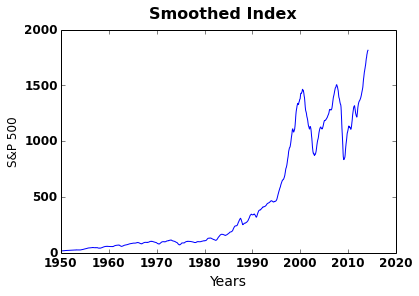
\includegraphics[max size={\textwidth}{\textheight}]{Final_Report_files/Final_Report_6_0.png}
    \par
    \end{center}
    
            \end{InvisibleVerbatim}
            
        
    
We tried to find the dates crises began and ended. We assumed that
crises began when bubbles were severe. In other words, the highest value
during a period of time and would be the starting date of crisis. But
the problem is, the index data is so volatile that there are so many
maxima. As a consequence, we rather use smoothing technique to estimate
a general pattern and then pick the maxima. By k-nearest neighbor
method, we estimated local maxima and chose the period we were using for
further analysis. The plot shows the result. Now we can see that it has
more smooth shape that we can pick maxima and minima.\subsection{Find max and min index}\label{find-max-and-min-index}

    % Make sure that atleast 4 lines are below the HR
    \needspace{4\baselineskip}

    
        \vspace{6pt}
        \makebox[0.1\linewidth]{\smaller\hfill\tt\color{nbframe-in-prompt}In\hspace{4pt}{[}59{]}:\hspace{4pt}}\\*
        \vspace{-2.65\baselineskip}
        \begin{ColorVerbatim}
            \vspace{-0.7\baselineskip}
            \begin{Verbatim}[commandchars=\\\{\}]
\PY{n}{maxprice} \PY{o}{=} \PY{n+nb}{range}\PY{p}{(}\PY{l+m+mi}{0}\PY{p}{)}
\PY{n}{maxdate} \PY{o}{=} \PY{n+nb}{range}\PY{p}{(}\PY{l+m+mi}{0}\PY{p}{)}
\PY{n}{maxobs} \PY{o}{=} \PY{n+nb}{range}\PY{p}{(}\PY{l+m+mi}{0}\PY{p}{)}
\PY{k}{for} \PY{n}{i} \PY{o+ow}{in} \PY{n+nb}{range}\PY{p}{(}\PY{l+m+mi}{16143}\PY{p}{)}\PY{p}{:}
	\PY{n}{maxi} \PY{o}{=} \PY{l+m+mi}{0}
	\PY{k}{if} \PY{n}{i}\PY{o}{\PYZhy{}}\PY{l+m+mi}{180} \PY{o}{\PYZlt{}} \PY{l+m+mi}{0}\PY{p}{:}
		\PY{n}{a} \PY{o}{=} \PY{n}{sprice}\PY{p}{[}\PY{l+m+mi}{0}\PY{p}{:}\PY{n}{i}\PY{o}{\PYZhy{}}\PY{l+m+mi}{1}\PY{p}{]} \PY{o}{+} \PY{n}{sprice}\PY{p}{[}\PY{n}{i}\PY{o}{+}\PY{l+m+mi}{1}\PY{p}{:}\PY{n}{i}\PY{o}{+}\PY{l+m+mi}{180}\PY{p}{]}
	\PY{k}{else}\PY{p}{:}
		\PY{k}{if} \PY{n}{i}\PY{o}{+}\PY{l+m+mi}{180} \PY{o}{\PYZgt{}} \PY{l+m+mi}{16142}\PY{p}{:}
			\PY{n}{a} \PY{o}{=} \PY{n}{sprice}\PY{p}{[}\PY{n}{i}\PY{o}{\PYZhy{}}\PY{l+m+mi}{180}\PY{p}{:}\PY{n}{i}\PY{o}{\PYZhy{}}\PY{l+m+mi}{1}\PY{p}{]} \PY{o}{+} \PY{n}{sprice}\PY{p}{[}\PY{n}{i}\PY{o}{+}\PY{l+m+mi}{1}\PY{p}{:}\PY{l+m+mi}{16142}\PY{p}{]}
		\PY{k}{else}\PY{p}{:}
			\PY{n}{a} \PY{o}{=} \PY{n}{sprice}\PY{p}{[}\PY{n}{i}\PY{o}{\PYZhy{}}\PY{l+m+mi}{180}\PY{p}{:}\PY{n}{i}\PY{o}{\PYZhy{}}\PY{l+m+mi}{1}\PY{p}{]} \PY{o}{+} \PY{n}{sprice}\PY{p}{[}\PY{n}{i}\PY{o}{+}\PY{l+m+mi}{1}\PY{p}{:}\PY{n}{i}\PY{o}{+}\PY{l+m+mi}{180}\PY{p}{]}
	\PY{k}{for} \PY{n}{number} \PY{o+ow}{in} \PY{n}{a}\PY{p}{:}
		\PY{k}{if} \PY{n}{number} \PY{o}{\PYZgt{}} \PY{n}{maxi}\PY{p}{:}
			\PY{n}{maxi} \PY{o}{=} \PY{n}{number}
	\PY{k}{if} \PY{n}{sprice}\PY{p}{[}\PY{n}{i}\PY{p}{]} \PY{o}{\PYZgt{}} \PY{n}{maxi}\PY{p}{:}
		\PY{n}{maxprice} \PY{o}{=} \PY{n}{maxprice} \PY{o}{+} \PY{p}{[}\PY{n}{sprice}\PY{p}{[}\PY{n}{i}\PY{p}{]}\PY{p}{]}
		\PY{n}{maxdate} \PY{o}{=} \PY{n}{maxdate} \PY{o}{+} \PY{p}{[}\PY{n}{numdate}\PY{p}{[}\PY{n}{i}\PY{p}{]}\PY{p}{]}
		\PY{n}{maxobs} \PY{o}{=} \PY{n}{maxobs} \PY{o}{+} \PY{p}{[}\PY{n}{i}\PY{p}{]}

\PY{n}{minprice} \PY{o}{=} \PY{n+nb}{range}\PY{p}{(}\PY{l+m+mi}{0}\PY{p}{)}
\PY{n}{mindate} \PY{o}{=} \PY{n+nb}{range}\PY{p}{(}\PY{l+m+mi}{0}\PY{p}{)}
\PY{n}{minobs} \PY{o}{=} \PY{n+nb}{range}\PY{p}{(}\PY{l+m+mi}{0}\PY{p}{)}
\PY{k}{for} \PY{n}{i} \PY{o+ow}{in} \PY{n+nb}{range}\PY{p}{(}\PY{l+m+mi}{16143}\PY{p}{)}\PY{p}{:}
	\PY{n}{mini} \PY{o}{=} \PY{l+m+mi}{2000}
	\PY{k}{if} \PY{n}{i}\PY{o}{\PYZhy{}}\PY{l+m+mi}{180} \PY{o}{\PYZlt{}} \PY{l+m+mi}{0}\PY{p}{:}
		\PY{n}{a} \PY{o}{=} \PY{n}{sprice}\PY{p}{[}\PY{l+m+mi}{0}\PY{p}{:}\PY{n}{i}\PY{o}{\PYZhy{}}\PY{l+m+mi}{1}\PY{p}{]} \PY{o}{+} \PY{n}{sprice}\PY{p}{[}\PY{n}{i}\PY{o}{+}\PY{l+m+mi}{1}\PY{p}{:}\PY{n}{i}\PY{o}{+}\PY{l+m+mi}{180}\PY{p}{]}
	\PY{k}{else}\PY{p}{:}
		\PY{k}{if} \PY{n}{i}\PY{o}{+}\PY{l+m+mi}{180} \PY{o}{\PYZgt{}} \PY{l+m+mi}{16142}\PY{p}{:}
			\PY{n}{a} \PY{o}{=} \PY{n}{sprice}\PY{p}{[}\PY{n}{i}\PY{o}{\PYZhy{}}\PY{l+m+mi}{180}\PY{p}{:}\PY{n}{i}\PY{o}{\PYZhy{}}\PY{l+m+mi}{1}\PY{p}{]} \PY{o}{+} \PY{n}{sprice}\PY{p}{[}\PY{n}{i}\PY{o}{+}\PY{l+m+mi}{1}\PY{p}{:}\PY{l+m+mi}{16142}\PY{p}{]}
		\PY{k}{else}\PY{p}{:}
			\PY{n}{a} \PY{o}{=} \PY{n}{sprice}\PY{p}{[}\PY{n}{i}\PY{o}{\PYZhy{}}\PY{l+m+mi}{180}\PY{p}{:}\PY{n}{i}\PY{o}{\PYZhy{}}\PY{l+m+mi}{1}\PY{p}{]} \PY{o}{+} \PY{n}{sprice}\PY{p}{[}\PY{n}{i}\PY{o}{+}\PY{l+m+mi}{1}\PY{p}{:}\PY{n}{i}\PY{o}{+}\PY{l+m+mi}{180}\PY{p}{]}
	\PY{k}{for} \PY{n}{number} \PY{o+ow}{in} \PY{n}{a}\PY{p}{:}
		\PY{k}{if} \PY{n}{number} \PY{o}{\PYZlt{}} \PY{n}{mini}\PY{p}{:}
			\PY{n}{mini} \PY{o}{=} \PY{n}{number}
	\PY{k}{if} \PY{n}{sprice}\PY{p}{[}\PY{n}{i}\PY{p}{]} \PY{o}{\PYZlt{}} \PY{n}{mini}\PY{p}{:}
		\PY{n}{minprice} \PY{o}{=} \PY{n}{minprice} \PY{o}{+} \PY{p}{[}\PY{n}{sprice}\PY{p}{[}\PY{n}{i}\PY{p}{]}\PY{p}{]}
		\PY{n}{mindate} \PY{o}{=} \PY{n}{mindate} \PY{o}{+} \PY{p}{[}\PY{n}{numdate}\PY{p}{[}\PY{n}{i}\PY{p}{]}\PY{p}{]}
		\PY{n}{minobs} \PY{o}{=} \PY{n}{minobs} \PY{o}{+} \PY{p}{[}\PY{n}{i}\PY{p}{]}

\PY{n}{fig} \PY{o}{=} \PY{n}{plt}\PY{o}{.}\PY{n}{figure}\PY{p}{(}\PY{p}{)}
\PY{n}{plt}\PY{o}{.}\PY{n}{plot}\PY{p}{(}\PY{n}{numdate}\PY{p}{,}\PY{n}{sprice}\PY{p}{)}
\PY{n}{plt}\PY{o}{.}\PY{n}{plot}\PY{p}{(}\PY{n}{maxdate}\PY{p}{,} \PY{n}{maxprice}\PY{p}{,} \PY{l+s}{\PYZdq{}}\PY{l+s}{o}\PY{l+s}{\PYZdq{}}\PY{p}{,} \PY{n}{label}\PY{o}{=}\PY{l+s}{\PYZdq{}}\PY{l+s}{max}\PY{l+s}{\PYZdq{}}\PY{p}{)}
\PY{n}{plt}\PY{o}{.}\PY{n}{plot}\PY{p}{(}\PY{n}{mindate}\PY{p}{,} \PY{n}{minprice}\PY{p}{,} \PY{l+s}{\PYZdq{}}\PY{l+s}{o}\PY{l+s}{\PYZdq{}}\PY{p}{,} \PY{n}{label}\PY{o}{=}\PY{l+s}{\PYZdq{}}\PY{l+s}{min}\PY{l+s}{\PYZdq{}}\PY{p}{)}
\PY{n}{plt}\PY{o}{.}\PY{n}{legend}\PY{p}{(}\PY{n}{loc}\PY{o}{=}\PY{l+m+mi}{0}\PY{p}{)}
\PY{n}{fig}\PY{o}{.}\PY{n}{suptitle}\PY{p}{(}\PY{l+s}{\PYZsq{}}\PY{l+s}{Smoothed Index}\PY{l+s}{\PYZsq{}}\PY{p}{,} \PY{n}{fontsize}\PY{o}{=}\PY{l+m+mi}{16}\PY{p}{)}
\PY{n}{plt}\PY{o}{.}\PY{n}{xlabel}\PY{p}{(}\PY{l+s}{\PYZsq{}}\PY{l+s}{Years}\PY{l+s}{\PYZsq{}}\PY{p}{,} \PY{n}{fontsize}\PY{o}{=}\PY{l+m+mi}{14}\PY{p}{)}
\PY{n}{plt}\PY{o}{.}\PY{n}{ylabel}\PY{p}{(}\PY{l+s}{\PYZsq{}}\PY{l+s}{S\PYZam{}P 500}\PY{l+s}{\PYZsq{}}\PY{p}{,} \PY{n}{fontsize}\PY{o}{=}\PY{l+m+mi}{12}\PY{p}{)}
\PY{n}{fig}\PY{o}{.}\PY{n}{savefig}\PY{p}{(}\PY{l+s}{\PYZsq{}}\PY{l+s}{test.jpg}\PY{l+s}{\PYZsq{}}\PY{p}{)}
\end{Verbatim}

            
                \vspace{-0.2\baselineskip}
            
        \end{ColorVerbatim}
    

    

        % If the first block is an image, minipage the image.  Else
        % request a certain amount of space for the input text.
        \needspace{4\baselineskip}
        
        

            % Add document contents.
            
                \begin{InvisibleVerbatim}
                \vspace{-0.5\baselineskip}
    \begin{center}
    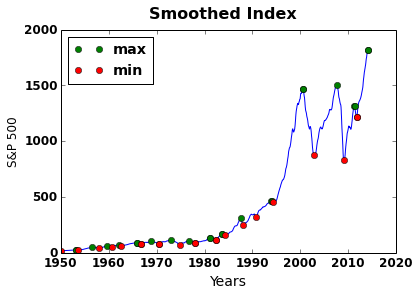
\includegraphics[max size={\textwidth}{\textheight}]{Final_Report_files/Final_Report_9_0.png}
    \par
    \end{center}
    
            \end{InvisibleVerbatim}
            
        
    
Based on dates when crises start, we cut off two different eras
supposedly possessing different characteristics. The first period was
from Jun 16th, 2000 to August 10th, 2007. The index during this period
was closely related to so-called the Dot-com bubble. The other period
started from August 11th, 2007 to May 2nd, 2011. That was related to the
recent financial crisis mainly because of the serial credit defaults in
the subprime mortgages.\subsection{Movements of S\&P 500 Daily
Price}\label{movements-of-sp-500-daily-price}

    % Make sure that atleast 4 lines are below the HR
    \needspace{4\baselineskip}

    
        \vspace{6pt}
        \makebox[0.1\linewidth]{\smaller\hfill\tt\color{nbframe-in-prompt}In\hspace{4pt}{[}60{]}:\hspace{4pt}}\\*
        \vspace{-2.65\baselineskip}
        \begin{ColorVerbatim}
            \vspace{-0.7\baselineskip}
            \begin{Verbatim}[commandchars=\\\{\}]
\PY{n}{rreturn} \PY{o}{=} \PY{n+nb}{range}\PY{p}{(}\PY{n+nb}{len}\PY{p}{(}\PY{n}{price}\PY{p}{)}\PY{o}{\PYZhy{}}\PY{l+m+mi}{1}\PY{p}{)}
\PY{k}{for} \PY{n}{i} \PY{o+ow}{in} \PY{n+nb}{range}\PY{p}{(}\PY{n+nb}{len}\PY{p}{(}\PY{n}{price}\PY{p}{)}\PY{o}{\PYZhy{}}\PY{l+m+mi}{1}\PY{p}{)}\PY{p}{:}
	\PY{n}{rreturn}\PY{p}{[}\PY{n}{i}\PY{p}{]}\PY{o}{=}\PY{p}{(}\PY{n}{price}\PY{p}{[}\PY{n}{i}\PY{o}{+}\PY{l+m+mi}{1}\PY{p}{]} \PY{o}{\PYZhy{}} \PY{n}{price}\PY{p}{[}\PY{n}{i}\PY{p}{]}\PY{p}{)}\PY{o}{/}\PY{n}{price}\PY{p}{[}\PY{n}{i}\PY{p}{]}

\PY{n}{preev} \PY{o}{=} \PY{n}{price}\PY{p}{[}\PY{l+m+mi}{12697}\PY{p}{:}\PY{l+m+mi}{14493}\PY{p}{]}
\PY{n}{postev} \PY{o}{=} \PY{n}{price}\PY{p}{[}\PY{l+m+mi}{14494}\PY{p}{:}\PY{l+m+mi}{15431}\PY{p}{]}

\PY{n}{prerr} \PY{o}{=} \PY{n}{rreturn}\PY{p}{[}\PY{l+m+mi}{12697}\PY{p}{:}\PY{l+m+mi}{14493}\PY{p}{]}
\PY{n}{postrr} \PY{o}{=} \PY{n}{rreturn}\PY{p}{[}\PY{l+m+mi}{14494}\PY{p}{:}\PY{l+m+mi}{15430}\PY{p}{]}

\PY{n}{predate} \PY{o}{=} \PY{n}{numdate}\PY{p}{[}\PY{l+m+mi}{12697}\PY{p}{:}\PY{l+m+mi}{14493}\PY{p}{]}
\PY{n}{postdate} \PY{o}{=} \PY{n}{numdate}\PY{p}{[}\PY{l+m+mi}{14494}\PY{p}{:}\PY{l+m+mi}{15431}\PY{p}{]}

\PY{n}{fig} \PY{o}{=} \PY{n}{plt}\PY{o}{.}\PY{n}{figure}\PY{p}{(}\PY{p}{)}
\PY{n}{plt}\PY{o}{.}\PY{n}{plot}\PY{p}{(}\PY{n}{predate}\PY{o}{+}\PY{n}{postdate}\PY{p}{,}\PY{n}{preev}\PY{o}{+}\PY{n}{postev}\PY{p}{)}
\PY{n}{plt}\PY{o}{.}\PY{n}{axvline}\PY{p}{(}\PY{n}{maxdate}\PY{p}{[}\PY{n+nb}{len}\PY{p}{(}\PY{n}{maxdate}\PY{p}{)}\PY{o}{\PYZhy{}}\PY{l+m+mi}{5}\PY{p}{]}\PY{p}{,} \PY{n}{color}\PY{o}{=}\PY{l+s}{\PYZsq{}}\PY{l+s}{k}\PY{l+s}{\PYZsq{}}\PY{p}{)}
\PY{n}{fig}\PY{o}{.}\PY{n}{suptitle}\PY{p}{(}\PY{l+s}{\PYZsq{}}\PY{l+s}{Truncated Index}\PY{l+s}{\PYZsq{}}\PY{p}{,} \PY{n}{fontsize}\PY{o}{=}\PY{l+m+mi}{16}\PY{p}{)}
\PY{n}{plt}\PY{o}{.}\PY{n}{xlabel}\PY{p}{(}\PY{l+s}{\PYZsq{}}\PY{l+s}{Years}\PY{l+s}{\PYZsq{}}\PY{p}{,} \PY{n}{fontsize}\PY{o}{=}\PY{l+m+mi}{14}\PY{p}{)}
\PY{n}{plt}\PY{o}{.}\PY{n}{ylabel}\PY{p}{(}\PY{l+s}{\PYZsq{}}\PY{l+s}{S\PYZam{}P 500}\PY{l+s}{\PYZsq{}}\PY{p}{,} \PY{n}{fontsize}\PY{o}{=}\PY{l+m+mi}{12}\PY{p}{)}
\PY{n}{fig}\PY{o}{.}\PY{n}{savefig}\PY{p}{(}\PY{l+s}{\PYZsq{}}\PY{l+s}{test.jpg}\PY{l+s}{\PYZsq{}}\PY{p}{)}
\end{Verbatim}

            
                \vspace{-0.2\baselineskip}
            
        \end{ColorVerbatim}
    

    

        % If the first block is an image, minipage the image.  Else
        % request a certain amount of space for the input text.
        \needspace{4\baselineskip}
        
        

            % Add document contents.
            
                \begin{InvisibleVerbatim}
                \vspace{-0.5\baselineskip}
    \begin{center}
    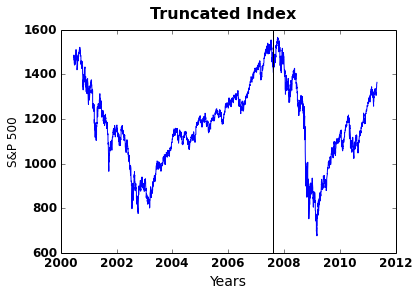
\includegraphics[max size={\textwidth}{\textheight}]{Final_Report_files/Final_Report_12_0.png}
    \par
    \end{center}
    
            \end{InvisibleVerbatim}
            
        
    
This plot shows the index during the two partitioned periods. Just
looking the two periods does not give many intuitive ideas whether they
are different in any senses, for example, the second period might be
more volatile than the other. We only can claim that from this plot that
the economic cycle was going to be short. In other words, the economy
may encounter crisis and bubble more frequently than before. We are now
using some time series data for further analysis.As we can see form the plot of stock prices, price movement doesn't have
an apparent pattern. The index really screwed up and hit the buttom
during the 2008 crisis. After that, it started to go up again. I almost
climbed over 1400 near the starting point but still carried with big
fluctuations. The variance of the stock price seems more volatile for
post-event.\subsection{Implementation of Autoregressive Integrated Moving Average
Model}\label{implementation-of-autoregressive-integrated-moving-average-model}We want, at this step, to get a general view and better understanding of
pre-event and post-event time series, to see if they are indeed of
different nature. We intend to implement the Autoregressive Integrated
Moving Average Model. In this way, not only could we get specific
formulas describing each of the time series that serve as an accurate
foundation for our argument, and it would allow us to do some
predictions and simulations on each data set. To simplify, we take just
one level of difference, d=1, in ARIMA Model.

    % Make sure that atleast 4 lines are below the HR
    \needspace{4\baselineskip}

    
        \vspace{6pt}
        \makebox[0.1\linewidth]{\smaller\hfill\tt\color{nbframe-in-prompt}In\hspace{4pt}{[}61{]}:\hspace{4pt}}\\*
        \vspace{-2.65\baselineskip}
        \begin{ColorVerbatim}
            \vspace{-0.7\baselineskip}
            \begin{Verbatim}[commandchars=\\\{\}]
\PY{k+kn}{import} \PY{n+nn}{statsmodels.api} \PY{k+kn}{as} \PY{n+nn}{sm}
\PY{k+kn}{from} \PY{n+nn}{statsmodels} \PY{k+kn}{import} \PY{o}{*}
\PY{n}{modelpre} \PY{o}{=} \PY{n}{tsa}\PY{o}{.}\PY{n}{arima\PYZus{}model}\PY{o}{.}\PY{n}{ARIMA}\PY{p}{(}\PY{n}{preev}\PY{p}{,} \PY{p}{[}\PY{l+m+mi}{1}\PY{p}{,} \PY{l+m+mi}{0}\PY{p}{,} \PY{l+m+mi}{1}\PY{p}{]}\PY{p}{,}\PY{n}{freq}\PY{o}{=}\PY{l+s}{\PYZsq{}}\PY{l+s}{M}\PY{l+s}{\PYZsq{}}\PY{p}{)}\PY{o}{.}\PY{n}{fit}\PY{p}{(}\PY{p}{)}
\PY{n}{modelpost} \PY{o}{=} \PY{n}{tsa}\PY{o}{.}\PY{n}{arima\PYZus{}model}\PY{o}{.}\PY{n}{ARIMA}\PY{p}{(}\PY{n}{postev}\PY{p}{,} \PY{p}{[}\PY{l+m+mi}{1}\PY{p}{,} \PY{l+m+mi}{1}\PY{p}{,} \PY{l+m+mi}{1}\PY{p}{]}\PY{p}{,}\PY{n}{freq}\PY{o}{=}\PY{l+s}{\PYZsq{}}\PY{l+s}{M}\PY{l+s}{\PYZsq{}}\PY{p}{)}\PY{o}{.}\PY{n}{fit}\PY{p}{(}\PY{p}{)}
\end{Verbatim}

            
                \vspace{-0.2\baselineskip}
            
        \end{ColorVerbatim}
    


    % Make sure that atleast 4 lines are below the HR
    \needspace{4\baselineskip}

    
        \vspace{6pt}
        \makebox[0.1\linewidth]{\smaller\hfill\tt\color{nbframe-in-prompt}In\hspace{4pt}{[}62{]}:\hspace{4pt}}\\*
        \vspace{-2.65\baselineskip}
        \begin{ColorVerbatim}
            \vspace{-0.7\baselineskip}
            \begin{Verbatim}[commandchars=\\\{\}]
\PY{n}{modelpre}\PY{o}{.}\PY{n}{summary}\PY{p}{(}\PY{p}{)} \PY{c}{\PYZsh{} Pre\PYZhy{}event model summary}
\end{Verbatim}

            
                \vspace{-0.2\baselineskip}
            
        \end{ColorVerbatim}
    

    

        % If the first block is an image, minipage the image.  Else
        % request a certain amount of space for the input text.
        \needspace{4\baselineskip}
        
        

            % Add document contents.
            
                \makebox[0.1\linewidth]{\smaller\hfill\tt\color{nbframe-out-prompt}Out\hspace{4pt}{[}62{]}:\hspace{4pt}}\\*
                \vspace{-2.55\baselineskip}\begin{InvisibleVerbatim}
                \vspace{-0.5\baselineskip}
\begin{alltt}<class 'statsmodels.iolib.summary.Summary'>
"""
                              ARMA Model Results
======================================================================
========
Dep. Variable:                      y   No. Observations:
1796
Model:                     ARMA(1, 1)   Log Likelihood
-7004.452
Method:                       css-mle   S.D. of innovations
11.936
Date:                Fri, 09 May 2014   AIC
14016.904
Time:                        03:19:54   BIC
14038.877
Sample:                             0   HQIC
14025.016

======================================================================
========
                 coef    std err          z      P>|z|      [95.0\%
Conf. Int.]
----------------------------------------------------------------------
--------
const       1292.5804    132.923      9.724      0.000      1032.056
1553.105
ar.L1.y        0.9983      0.001    811.567      0.000         0.996
1.001
ma.L1.y       -0.0424      0.025     -1.691      0.091        -0.092
0.007
                                    Roots
======================================================================
=======
                 Real           Imaginary           Modulus
Frequency
----------------------------------------------------------------------
-------
AR.1            1.0017           +0.0000j            1.0017
0.0000
MA.1           23.5871           +0.0000j           23.5871
0.0000
----------------------------------------------------------------------
-------
"""\end{alltt}

            \end{InvisibleVerbatim}
            
        
    


    % Make sure that atleast 4 lines are below the HR
    \needspace{4\baselineskip}

    
        \vspace{6pt}
        \makebox[0.1\linewidth]{\smaller\hfill\tt\color{nbframe-in-prompt}In\hspace{4pt}{[}63{]}:\hspace{4pt}}\\*
        \vspace{-2.65\baselineskip}
        \begin{ColorVerbatim}
            \vspace{-0.7\baselineskip}
            \begin{Verbatim}[commandchars=\\\{\}]
\PY{n}{modelpost}\PY{o}{.}\PY{n}{summary}\PY{p}{(}\PY{p}{)} \PY{c}{\PYZsh{}Post\PYZhy{}event model summary}
\end{Verbatim}

            
                \vspace{-0.2\baselineskip}
            
        \end{ColorVerbatim}
    

    

        % If the first block is an image, minipage the image.  Else
        % request a certain amount of space for the input text.
        \needspace{4\baselineskip}
        
        

            % Add document contents.
            
                \makebox[0.1\linewidth]{\smaller\hfill\tt\color{nbframe-out-prompt}Out\hspace{4pt}{[}63{]}:\hspace{4pt}}\\*
                \vspace{-2.55\baselineskip}\begin{InvisibleVerbatim}
                \vspace{-0.5\baselineskip}
\begin{alltt}<class 'statsmodels.iolib.summary.Summary'>
"""
                             ARIMA Model Results
======================================================================
========
Dep. Variable:                    D.y   No. Observations:
936
Model:                 ARIMA(1, 1, 1)   Log Likelihood
-4044.155
Method:                       css-mle   S.D. of innovations
18.206
Date:                Fri, 09 May 2014   AIC
8096.310
Time:                        03:19:56   BIC
8115.677
Sample:                             1   HQIC
8103.695

======================================================================
========
                 coef    std err          z      P>|z|      [95.0\%
Conf. Int.]
----------------------------------------------------------------------
--------
const         -0.0903      0.473     -0.191      0.849        -1.016
0.836
ar.L1.D.y      0.2611      0.153      1.712      0.087        -0.038
0.560
ma.L1.D.y     -0.4135      0.143     -2.893      0.004        -0.694
-0.133
                                    Roots
======================================================================
=======
                 Real           Imaginary           Modulus
Frequency
----------------------------------------------------------------------
-------
AR.1            3.8293           +0.0000j            3.8293
0.0000
MA.1            2.4186           +0.0000j            2.4186
0.0000
----------------------------------------------------------------------
-------
"""\end{alltt}

            \end{InvisibleVerbatim}
            
        
    
Actually, python has not enough packages to analyze time series data. So
we are using rpy2 to use some useful packages in R.

    % Make sure that atleast 4 lines are below the HR
    \needspace{4\baselineskip}

    
        \vspace{6pt}
        \makebox[0.1\linewidth]{\smaller\hfill\tt\color{nbframe-in-prompt}In\hspace{4pt}{[}64{]}:\hspace{4pt}}\\*
        \vspace{-2.65\baselineskip}
        \begin{ColorVerbatim}
            \vspace{-0.7\baselineskip}
            \begin{Verbatim}[commandchars=\\\{\}]
\PY{k+kn}{import} \PY{n+nn}{rpy2} \PY{k+kn}{as} \PY{n+nn}{rpy2}
\PY{o}{\PYZpc{}}\PY{k}{load\PYZus{}ext} \PY{n}{rmagic}
\end{Verbatim}

            
                \vspace{-0.2\baselineskip}
            
        \end{ColorVerbatim}
    

    

        % If the first block is an image, minipage the image.  Else
        % request a certain amount of space for the input text.
        \needspace{4\baselineskip}
        
        

            % Add document contents.
            
                \begin{InvisibleVerbatim}
                \vspace{-0.5\baselineskip}
\begin{alltt}The rmagic extension is already loaded. To reload it, use:
  \%reload\_ext rmagic
\end{alltt}

            \end{InvisibleVerbatim}
            
        
    


    % Make sure that atleast 4 lines are below the HR
    \needspace{4\baselineskip}

    
        \vspace{6pt}
        \makebox[0.1\linewidth]{\smaller\hfill\tt\color{nbframe-in-prompt}In\hspace{4pt}{[}65{]}:\hspace{4pt}}\\*
        \vspace{-2.65\baselineskip}
        \begin{ColorVerbatim}
            \vspace{-0.7\baselineskip}
            \begin{Verbatim}[commandchars=\\\{\}]
\PY{o}{\PYZpc{}\PYZpc{}}\PY{k}{R}
\PY{n}{install}\PY{o}{.}\PY{n}{packages}\PY{p}{(}\PY{l+s}{\PYZdq{}}\PY{l+s}{forecasting}\PY{l+s}{\PYZdq{}}\PY{p}{)}
\end{Verbatim}

            
                \vspace{-0.2\baselineskip}
            
        \end{ColorVerbatim}
    


    % Make sure that atleast 4 lines are below the HR
    \needspace{4\baselineskip}

    
        \vspace{6pt}
        \makebox[0.1\linewidth]{\smaller\hfill\tt\color{nbframe-in-prompt}In\hspace{4pt}{[}66{]}:\hspace{4pt}}\\*
        \vspace{-2.65\baselineskip}
        \begin{ColorVerbatim}
            \vspace{-0.7\baselineskip}
            \begin{Verbatim}[commandchars=\\\{\}]
\PY{o}{\PYZpc{}\PYZpc{}}\PY{k}{R}
\PY{n}{library}\PY{p}{(}\PY{l+s}{\PYZdq{}}\PY{l+s}{forecast}\PY{l+s}{\PYZdq{}}\PY{p}{)}
\end{Verbatim}

            
                \vspace{-0.2\baselineskip}
            
        \end{ColorVerbatim}
    
A list with component ar and/or ma giving the AR and MA coefficients
respectively. Optionally a component order can be used. An empty list
gives an ARIMA(0, 0, 0) model, that is white noise. n, length of output
series, before un-differencing. A strictly positive integer.

The ARIMA result tables are very detailed. The pre-event time series is
fitted with ARMA(1,1) model while ARIMA(1,1,1) is chosen for the
post-event time series. Each coefficient in both model has a very small
standard deviation error and p-value. We can see from the criteria that
the models fit pretty well. And since the resulting models are very
different, we can conclude that those two are indeed not similar time
series.\subsection{Forecast and Simulation}\label{forecast-and-simulation}The data sets in pre-event and post-event are both of limited sizes.
With the specific formulas obtained from the ARIMA model results, we
want to use the forecast and simulation functions to get a general
picture of the volatility difference between the two events in a larger
background of data.

    % Make sure that atleast 4 lines are below the HR
    \needspace{4\baselineskip}

    
        \vspace{6pt}
        \makebox[0.1\linewidth]{\smaller\hfill\tt\color{nbframe-in-prompt}In\hspace{4pt}{[}67{]}:\hspace{4pt}}\\*
        \vspace{-2.65\baselineskip}
        \begin{ColorVerbatim}
            \vspace{-0.7\baselineskip}
            \begin{Verbatim}[commandchars=\\\{\}]
\PY{o}{\PYZpc{}\PYZpc{}}\PY{k}{R} \PY{o}{\PYZhy{}}\PY{n}{o} \PY{n}{presim}
\PY{n}{presim} \PY{o}{\PYZlt{}}\PY{o}{\PYZhy{}} \PY{k}{as}\PY{o}{.}\PY{n}{vector}\PY{p}{(}\PY{n}{arima}\PY{o}{.}\PY{n}{sim}\PY{p}{(}\PY{n+nb}{list}\PY{p}{(}\PY{n}{order} \PY{o}{=} \PY{n}{c}\PY{p}{(}\PY{l+m+mi}{1}\PY{p}{,}\PY{l+m+mi}{0}\PY{p}{,}\PY{l+m+mi}{1}\PY{p}{)}\PY{p}{,} \PY{n}{ar} \PY{o}{=} \PY{l+m+mf}{0.9983}\PY{p}{,} \PY{n}{ma} \PY{o}{=} \PY{o}{\PYZhy{}}\PY{l+m+mf}{0.0424}\PY{p}{)}\PY{p}{,} \PY{n}{n} \PY{o}{=} \PY{l+m+mi}{200}\PY{p}{)}\PY{p}{)}
\end{Verbatim}

            
                \vspace{-0.2\baselineskip}
            
        \end{ColorVerbatim}
    


    % Make sure that atleast 4 lines are below the HR
    \needspace{4\baselineskip}

    
        \vspace{6pt}
        \makebox[0.1\linewidth]{\smaller\hfill\tt\color{nbframe-in-prompt}In\hspace{4pt}{[}68{]}:\hspace{4pt}}\\*
        \vspace{-2.65\baselineskip}
        \begin{ColorVerbatim}
            \vspace{-0.7\baselineskip}
            \begin{Verbatim}[commandchars=\\\{\}]
\PY{n}{plot}\PY{p}{(}\PY{n+nb}{range}\PY{p}{(}\PY{n+nb}{len}\PY{p}{(}\PY{n}{presim}\PY{p}{)}\PY{p}{)}\PY{p}{,} \PY{n}{presim}\PY{p}{)}
\end{Verbatim}

            
                \vspace{-0.2\baselineskip}
            
        \end{ColorVerbatim}
    

    

        % If the first block is an image, minipage the image.  Else
        % request a certain amount of space for the input text.
        \needspace{4\baselineskip}
        
        

            % Add document contents.
            
                \makebox[0.1\linewidth]{\smaller\hfill\tt\color{nbframe-out-prompt}Out\hspace{4pt}{[}68{]}:\hspace{4pt}}\\*
                \vspace{-2.55\baselineskip}\begin{InvisibleVerbatim}
                \vspace{-0.5\baselineskip}
\begin{alltt}[<matplotlib.lines.Line2D at 0x1084d3590>]\end{alltt}

            \end{InvisibleVerbatim}
            
                \begin{InvisibleVerbatim}
                \vspace{-0.5\baselineskip}
    \begin{center}
    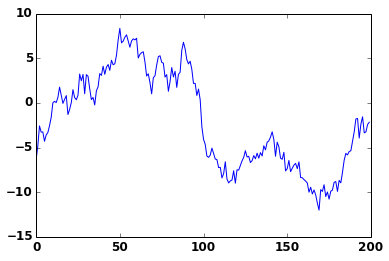
\includegraphics[max size={\textwidth}{\textheight}]{Final_Report_files/Final_Report_28_1.png}
    \par
    \end{center}
    
            \end{InvisibleVerbatim}
            
        
    


    % Make sure that atleast 4 lines are below the HR
    \needspace{4\baselineskip}

    
        \vspace{6pt}
        \makebox[0.1\linewidth]{\smaller\hfill\tt\color{nbframe-in-prompt}In\hspace{4pt}{[}69{]}:\hspace{4pt}}\\*
        \vspace{-2.65\baselineskip}
        \begin{ColorVerbatim}
            \vspace{-0.7\baselineskip}
            \begin{Verbatim}[commandchars=\\\{\}]
\PY{o}{\PYZpc{}\PYZpc{}}\PY{k}{R} \PY{o}{\PYZhy{}}\PY{n}{o} \PY{n}{postsim}
\PY{n}{postsim} \PY{o}{\PYZlt{}}\PY{o}{\PYZhy{}} \PY{k}{as}\PY{o}{.}\PY{n}{vector}\PY{p}{(}\PY{n}{arima}\PY{o}{.}\PY{n}{sim}\PY{p}{(}\PY{n+nb}{list}\PY{p}{(}\PY{n}{order} \PY{o}{=} \PY{n}{c}\PY{p}{(}\PY{l+m+mi}{1}\PY{p}{,}\PY{l+m+mi}{1}\PY{p}{,}\PY{l+m+mi}{1}\PY{p}{)}\PY{p}{,} \PY{n}{ar} \PY{o}{=} \PY{l+m+mf}{0.2611}\PY{p}{,} \PY{n}{ma} \PY{o}{=} \PY{o}{\PYZhy{}}\PY{l+m+mf}{0.4135}\PY{p}{)}\PY{p}{,} \PY{n}{n} \PY{o}{=} \PY{l+m+mi}{200}\PY{p}{)}\PY{p}{)}
\end{Verbatim}

            
                \vspace{-0.2\baselineskip}
            
        \end{ColorVerbatim}
    


    % Make sure that atleast 4 lines are below the HR
    \needspace{4\baselineskip}

    
        \vspace{6pt}
        \makebox[0.1\linewidth]{\smaller\hfill\tt\color{nbframe-in-prompt}In\hspace{4pt}{[}70{]}:\hspace{4pt}}\\*
        \vspace{-2.65\baselineskip}
        \begin{ColorVerbatim}
            \vspace{-0.7\baselineskip}
            \begin{Verbatim}[commandchars=\\\{\}]
\PY{n}{plot}\PY{p}{(}\PY{n+nb}{range}\PY{p}{(}\PY{n+nb}{len}\PY{p}{(}\PY{n}{postsim}\PY{p}{)}\PY{p}{)}\PY{p}{,} \PY{n}{postsim}\PY{p}{)}
\end{Verbatim}

            
                \vspace{-0.2\baselineskip}
            
        \end{ColorVerbatim}
    

    

        % If the first block is an image, minipage the image.  Else
        % request a certain amount of space for the input text.
        \needspace{4\baselineskip}
        
        

            % Add document contents.
            
                \makebox[0.1\linewidth]{\smaller\hfill\tt\color{nbframe-out-prompt}Out\hspace{4pt}{[}70{]}:\hspace{4pt}}\\*
                \vspace{-2.55\baselineskip}\begin{InvisibleVerbatim}
                \vspace{-0.5\baselineskip}
\begin{alltt}[<matplotlib.lines.Line2D at 0x111600dd0>]\end{alltt}

            \end{InvisibleVerbatim}
            
                \begin{InvisibleVerbatim}
                \vspace{-0.5\baselineskip}
    \begin{center}
    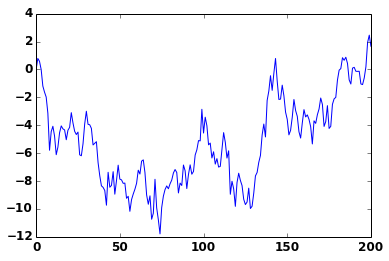
\includegraphics[max size={\textwidth}{\textheight}]{Final_Report_files/Final_Report_30_1.png}
    \par
    \end{center}
    
            \end{InvisibleVerbatim}
            
        
    
ARMA model in R environment from pre event data is made into the object
arimapre

    % Make sure that atleast 4 lines are below the HR
    \needspace{4\baselineskip}

    
        \vspace{6pt}
        \makebox[0.1\linewidth]{\smaller\hfill\tt\color{nbframe-in-prompt}In\hspace{4pt}{[}71{]}:\hspace{4pt}}\\*
        \vspace{-2.65\baselineskip}
        \begin{ColorVerbatim}
            \vspace{-0.7\baselineskip}
            \begin{Verbatim}[commandchars=\\\{\}]
\PY{o}{\PYZpc{}\PYZpc{}}\PY{k}{R} \PY{o}{\PYZhy{}}\PY{n}{i} \PY{n}{preev}
\PY{n}{library}\PY{p}{(}\PY{n}{stats}\PY{p}{)}
\PY{n}{arimapre} \PY{o}{\PYZlt{}}\PY{o}{\PYZhy{}} \PY{n}{arima}\PY{p}{(}\PY{n}{ts}\PY{p}{(}\PY{n}{preev}\PY{p}{)}\PY{p}{,}\PY{n}{c}\PY{p}{(}\PY{l+m+mi}{1}\PY{p}{,}\PY{l+m+mi}{0}\PY{p}{,}\PY{l+m+mi}{1}\PY{p}{)}\PY{p}{)}
\PY{k}{print}\PY{p}{(}\PY{n}{arimapre}\PY{p}{)}
\end{Verbatim}

            
                \vspace{-0.2\baselineskip}
            
        \end{ColorVerbatim}
    

    

        % If the first block is an image, minipage the image.  Else
        % request a certain amount of space for the input text.
        \needspace{4\baselineskip}
        
        

            % Add document contents.
            
                \begin{InvisibleVerbatim}
                \vspace{-0.5\baselineskip}
\begin{alltt}Series: ts(preev)
ARIMA(1,0,1) with non-zero mean

Coefficients:
         ar1      ma1  intercept
      0.9985  -0.0423  1185.8297
s.e.  0.0018   0.0251   187.6526

sigma\^{}2 estimated as 142.5:  log likelihood=-7004.82
AIC=14017.65   AICc=14017.67   BIC=14039.62
\end{alltt}

            \end{InvisibleVerbatim}
            
        
    
ARIMA model in R environment from post event data is made into the
object arimapost

    % Make sure that atleast 4 lines are below the HR
    \needspace{4\baselineskip}

    
        \vspace{6pt}
        \makebox[0.1\linewidth]{\smaller\hfill\tt\color{nbframe-in-prompt}In\hspace{4pt}{[}72{]}:\hspace{4pt}}\\*
        \vspace{-2.65\baselineskip}
        \begin{ColorVerbatim}
            \vspace{-0.7\baselineskip}
            \begin{Verbatim}[commandchars=\\\{\}]
\PY{o}{\PYZpc{}\PYZpc{}}\PY{k}{R} \PY{o}{\PYZhy{}}\PY{n}{i} \PY{n}{postev}
\PY{n}{arimapost} \PY{o}{\PYZlt{}}\PY{o}{\PYZhy{}} \PY{n}{arima}\PY{p}{(}\PY{n}{ts}\PY{p}{(}\PY{n}{postev}\PY{p}{)}\PY{p}{,}\PY{n}{c}\PY{p}{(}\PY{l+m+mi}{1}\PY{p}{,}\PY{l+m+mi}{1}\PY{p}{,}\PY{l+m+mi}{1}\PY{p}{)}\PY{p}{)}
\PY{k}{print}\PY{p}{(}\PY{n}{arimapost}\PY{p}{)}
\end{Verbatim}

            
                \vspace{-0.2\baselineskip}
            
        \end{ColorVerbatim}
    

    

        % If the first block is an image, minipage the image.  Else
        % request a certain amount of space for the input text.
        \needspace{4\baselineskip}
        
        

            % Add document contents.
            
                \begin{InvisibleVerbatim}
                \vspace{-0.5\baselineskip}
\begin{alltt}Series: ts(postev)
ARIMA(1,1,1)

Coefficients:
         ar1      ma1
      0.2610  -0.4133
s.e.  0.1525   0.1429

sigma\^{}2 estimated as 331.5:  log likelihood=-4044.17
AIC=8094.35   AICc=8094.37   BIC=8108.87
\end{alltt}

            \end{InvisibleVerbatim}
            
        
    
Here are plots to forecast from the two models

    % Make sure that atleast 4 lines are below the HR
    \needspace{4\baselineskip}

    
        \vspace{6pt}
        \makebox[0.1\linewidth]{\smaller\hfill\tt\color{nbframe-in-prompt}In\hspace{4pt}{[}73{]}:\hspace{4pt}}\\*
        \vspace{-2.65\baselineskip}
        \begin{ColorVerbatim}
            \vspace{-0.7\baselineskip}
            \begin{Verbatim}[commandchars=\\\{\}]
\PY{o}{\PYZpc{}\PYZpc{}}\PY{k}{R}
\PY{n}{library}\PY{p}{(}\PY{l+s}{\PYZdq{}}\PY{l+s}{forecast}\PY{l+s}{\PYZdq{}}\PY{p}{)}
\PY{n}{plot}\PY{p}{(}\PY{n}{forecast}\PY{p}{(}\PY{n+nb}{object}\PY{o}{=}\PY{n}{arimapre}\PY{p}{,} \PY{n}{h}\PY{o}{=}\PY{l+m+mi}{1000}\PY{p}{)}\PY{p}{)}
\PY{n}{plot}\PY{p}{(}\PY{n}{forecast}\PY{p}{(}\PY{n+nb}{object}\PY{o}{=}\PY{n}{arimapost}\PY{p}{,} \PY{n}{h}\PY{o}{=}\PY{l+m+mi}{1000}\PY{p}{)}\PY{p}{)}
\end{Verbatim}

            
                \vspace{-0.2\baselineskip}
            
        \end{ColorVerbatim}
    

    

        % If the first block is an image, minipage the image.  Else
        % request a certain amount of space for the input text.
        \needspace{4\baselineskip}
        
        

            % Add document contents.
            
                \begin{InvisibleVerbatim}
                \vspace{-0.5\baselineskip}
    \begin{center}
    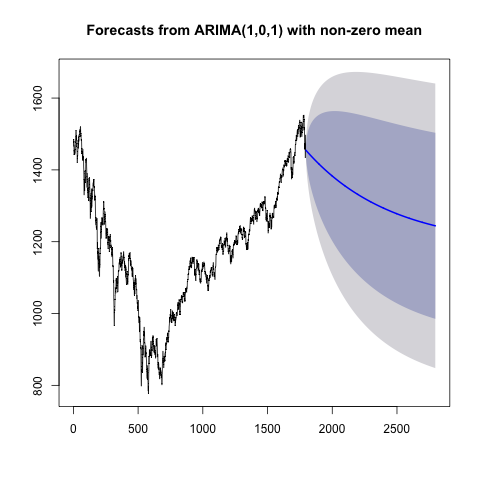
\includegraphics[max size={\textwidth}{\textheight}]{Final_Report_files/Final_Report_36_0.png}
    \par
    \end{center}
    
            \end{InvisibleVerbatim}
            
                \begin{InvisibleVerbatim}
                \vspace{-0.5\baselineskip}
    \begin{center}
    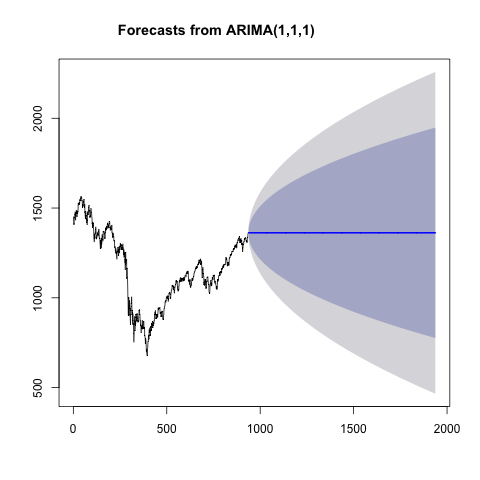
\includegraphics[max size={\textwidth}{\textheight}]{Final_Report_files/Final_Report_36_1.png}
    \par
    \end{center}
    
            \end{InvisibleVerbatim}
            
        
    
The forecast pictures clearly show an obvious difference in the standard
deviation of two events. The two forecast graphs are not in the same
unit. Pre-events' s standard errors is around 250 scale while
post-event's standard deviation is around 500. The simulation plots also
present post-event with larger volatility.\subsection{The Implementation of Generalized AutoRegressive Conditional
Heteroskedasticity
Model}\label{the-implementation-of-generalized-autoregressive-conditional-heteroskedasticity-model}As studies show, the asymmetric nature of information and pricing, the
heteroscedasticity, suggests the use of nonlinear time series structures
to model the attitude of investors toward risk and ex- pected return.
For example, Bera and Higgins (1993, p.315) remarked that ``a major
contribution of the ARCH literature is the finding that apparent changes
in the volatility of economic time series may be predictable and result
from a specific type of nonlinear dependence rather than exogenous
structural changes in variables.'' Here, in the case of financial data,
large and small errors tend to occur in clusters, i.e., large returns
are followed by more large returns, and small returns by more small
returns. This character of volatility clustering will be show in the
section of log return plots. This suggests that returns are serially
correlated.

To address the previous observed dynamic pattern volatility change, we
introduce the generalized autoregressive conditional heteroskedasticity
model. Shocks are assumed to be random, GARCH uses a nonlinear function
relating the observed time series and the underlying shocks. Since in
GARCH model conditional variance is dependent on its own previous lags,
the volatility clustering shown by the previous plots would be
characterized. The following resulting functions identify the different
nature of the events' volatilities.Summary statistics from GARCH model This shows volatility from pre event
data

    % Make sure that atleast 4 lines are below the HR
    \needspace{4\baselineskip}

    
        \vspace{6pt}
        \makebox[0.1\linewidth]{\smaller\hfill\tt\color{nbframe-in-prompt}In\hspace{4pt}{[}74{]}:\hspace{4pt}}\\*
        \vspace{-2.65\baselineskip}
        \begin{ColorVerbatim}
            \vspace{-0.7\baselineskip}
            \begin{Verbatim}[commandchars=\\\{\}]
\PY{o}{\PYZpc{}\PYZpc{}}\PY{k}{R}
\PY{n}{install}\PY{o}{.}\PY{n}{packages}\PY{p}{(}\PY{l+s}{\PYZdq{}}\PY{l+s}{tseries}\PY{l+s}{\PYZdq{}}\PY{p}{)}
\PY{n}{library}\PY{p}{(}\PY{l+s}{\PYZdq{}}\PY{l+s}{tseries}\PY{l+s}{\PYZdq{}}\PY{p}{)}
\PY{n}{dat1} \PY{o}{\PYZlt{}}\PY{o}{\PYZhy{}} \PY{n}{diff}\PY{p}{(}\PY{n}{log}\PY{p}{(}\PY{n}{preev}\PY{p}{)}\PY{p}{)}
\PY{n}{dat1} \PY{o}{\PYZlt{}}\PY{o}{\PYZhy{}} \PY{n}{ts}\PY{p}{(}\PY{n}{dat1}\PY{p}{)}
\PY{n}{dat1}\PY{o}{.}\PY{n}{garch} \PY{o}{\PYZlt{}}\PY{o}{\PYZhy{}} \PY{n}{garch}\PY{p}{(}\PY{n}{dat1}\PY{p}{)}
\PY{n}{summary}\PY{p}{(}\PY{n}{dat1}\PY{o}{.}\PY{n}{garch}\PY{p}{)}
\PY{n}{plot}\PY{p}{(}\PY{n}{dat1}\PY{o}{.}\PY{n}{garch}\PY{p}{)} 
\end{Verbatim}

            
                \vspace{-0.2\baselineskip}
            
        \end{ColorVerbatim}
    

    

        % If the first block is an image, minipage the image.  Else
        % request a certain amount of space for the input text.
        \needspace{4\baselineskip}
        
        

            % Add document contents.
            
                \begin{InvisibleVerbatim}
                \vspace{-0.5\baselineskip}
\begin{alltt}Hit <Return> to see next plot:
Hit <Return> to see next plot:
Hit <Return> to see next plot:
Hit <Return> to see next plot:
\end{alltt}

            \end{InvisibleVerbatim}
            
                \begin{InvisibleVerbatim}
                \vspace{-0.5\baselineskip}
\begin{alltt}trying URL 'http://cran.cnr.Berkeley.edu/bin/macosx/contrib/3.0/tserie
s\_0.10-32.tgz'
Content type 'application/x-gzip' length 308854 bytes (301 Kb)
opened URL
==================================================
downloaded 301 Kb


The downloaded binary packages are in
        /var/folders/vc/r5p1rx6x1275xdrjkcfv2mlc0000gn/T//RtmpAMAR0T/d
ownloaded\_packages

 ***** ESTIMATION WITH ANALYTICAL GRADIENT *****


     I     INITIAL X(I)        D(I)

     1     1.033614e-04     1.000e+00
     2     5.000000e-02     1.000e+00
     3     5.000000e-02     1.000e+00

    IT   NF      F         RELDF    PRELDF    RELDX   STPPAR   D*STEP
NPRELDF
     0    1 -7.270e+03
     1    7 -7.270e+03  5.41e-05  5.75e-04  1.0e-04  4.2e+10  1.0e-05
1.20e+07
     2    8 -7.271e+03  1.13e-04  1.30e-04  4.8e-05  2.0e+00  5.0e-06
1.32e+01
     3    9 -7.271e+03  1.58e-06  1.48e-06  4.9e-05  2.0e+00  5.0e-06
1.33e+01
     4   17 -7.296e+03  3.37e-03  4.95e-03  4.5e-01  2.0e+00  8.2e-02
1.33e+01
     5   20 -7.361e+03  8.89e-03  7.72e-03  7.2e-01  2.0e+00  3.3e-01
2.35e+00
     6   22 -7.383e+03  2.98e-03  2.31e-03  7.7e-02  2.0e+00  6.6e-02
4.02e+00
     7   24 -7.423e+03  5.36e-03  5.63e-03  1.3e-01  2.0e+00  1.3e-01
5.75e+01
     8   26 -7.435e+03  1.68e-03  2.19e-03  4.7e-02  2.0e+00  5.8e-02
4.07e+01
     9   27 -7.441e+03  7.64e-04  2.26e-03  4.3e-02  2.0e+00  5.8e-02
5.00e+00
    10   29 -7.443e+03  2.94e-04  9.30e-04  7.1e-03  2.0e+00  1.0e-02
5.96e-01
    11   30 -7.445e+03  2.81e-04  4.77e-04  7.1e-03  2.0e+00  1.0e-02
2.31e-03
    12   31 -7.445e+03  4.30e-05  6.41e-05  7.0e-03  2.0e+00  1.0e-02
8.77e-03
    13   33 -7.445e+03  7.87e-07  1.74e-05  1.9e-03  2.0e+00  2.7e-03
7.74e-03
    14   34 -7.446e+03  1.55e-05  1.90e-05  9.8e-04  2.0e+00  1.4e-03
1.49e-03
    15   38 -7.461e+03  2.06e-03  1.02e-03  3.9e-02  0.0e+00  7.3e-02
1.02e-03
    16   40 -7.463e+03  2.82e-04  4.63e-04  1.9e-02  1.9e+00  2.9e-02
1.49e-02
    17   43 -7.488e+03  3.29e-03  3.28e-03  5.6e-02  1.1e+00  1.2e-01
3.55e-02
    18   45 -7.490e+03  2.50e-04  8.52e-04  1.1e-02  1.9e+00  2.3e-02
1.64e-02
    19   46 -7.497e+03  9.62e-04  9.86e-04  1.1e-02  1.9e+00  2.3e-02
1.22e-02
    20   48 -7.500e+03  4.20e-04  4.78e-04  1.0e-02  1.3e+00  2.3e-02
6.38e-03
    21   49 -7.502e+03  2.42e-04  3.06e-04  1.1e-02  1.2e+00  2.3e-02
9.78e-04
    22   50 -7.503e+03  1.33e-04  2.65e-04  9.4e-03  9.4e-01  2.3e-02
4.48e-04
    23   51 -7.503e+03  6.81e-06  2.54e-05  1.4e-03  0.0e+00  3.1e-03
2.54e-05
    24   52 -7.503e+03  7.75e-06  1.53e-05  1.5e-03  6.5e-01  3.1e-03
1.60e-05
    25   53 -7.503e+03  1.57e-06  4.89e-06  7.2e-04  0.0e+00  1.4e-03
4.89e-06
    26   54 -7.503e+03  1.60e-06  1.59e-06  6.6e-04  2.7e-02  1.4e-03
1.59e-06
    27   55 -7.503e+03  4.77e-09  7.95e-09  4.0e-05  0.0e+00  9.5e-05
7.95e-09
    28   56 -7.503e+03  2.93e-10  4.73e-10  1.4e-05  0.0e+00  3.7e-05
4.73e-10
    29   57 -7.503e+03  5.21e-11  1.42e-12  9.9e-07  0.0e+00  2.2e-06
1.42e-12
    30   58 -7.503e+03 -4.37e-12  1.12e-14  6.1e-08  0.0e+00  1.3e-07
1.12e-14

 ***** RELATIVE FUNCTION CONVERGENCE *****

 FUNCTION    -7.502876e+03   RELDX        6.127e-08
 FUNC. EVALS      58         GRAD. EVALS      30
 PRELDF       1.120e-14      NPRELDF      1.120e-14

     I      FINAL X(I)        D(I)          G(I)

     1    1.120162e-06     1.000e+00     5.122e+01
     2    6.861711e-02     1.000e+00     7.346e-04
     3    9.211163e-01     1.000e+00     1.032e-03

\end{alltt}

            \end{InvisibleVerbatim}
            
                \begin{InvisibleVerbatim}
                \vspace{-0.5\baselineskip}
    \begin{center}
    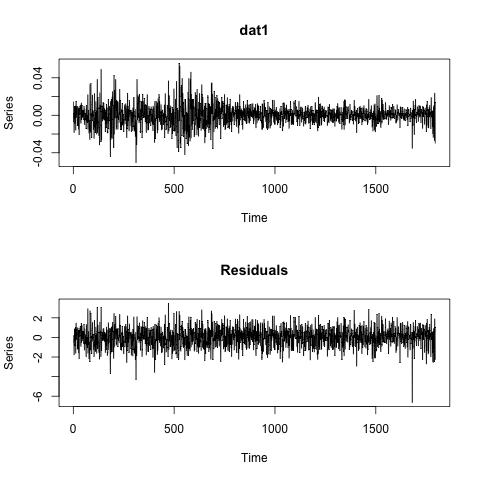
\includegraphics[max size={\textwidth}{\textheight}]{Final_Report_files/Final_Report_41_2.png}
    \par
    \end{center}
    
            \end{InvisibleVerbatim}
            
                \begin{InvisibleVerbatim}
                \vspace{-0.5\baselineskip}
    \begin{center}
    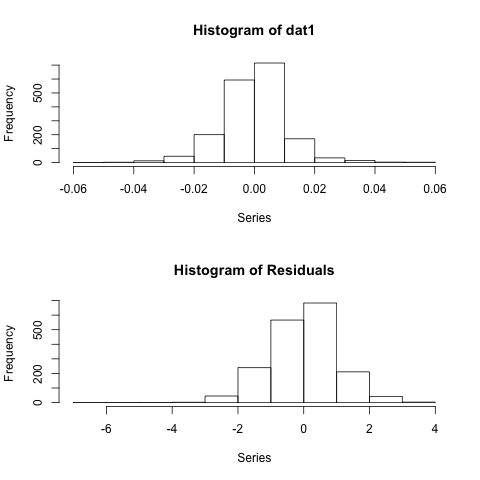
\includegraphics[max size={\textwidth}{\textheight}]{Final_Report_files/Final_Report_41_3.png}
    \par
    \end{center}
    
            \end{InvisibleVerbatim}
            
                \begin{InvisibleVerbatim}
                \vspace{-0.5\baselineskip}
    \begin{center}
    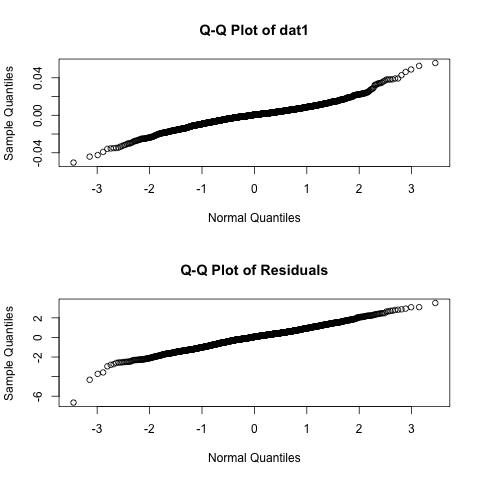
\includegraphics[max size={\textwidth}{\textheight}]{Final_Report_files/Final_Report_41_4.png}
    \par
    \end{center}
    
            \end{InvisibleVerbatim}
            
                \begin{InvisibleVerbatim}
                \vspace{-0.5\baselineskip}
    \begin{center}
    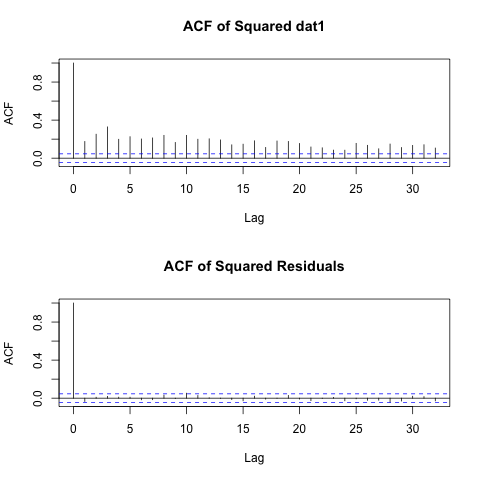
\includegraphics[max size={\textwidth}{\textheight}]{Final_Report_files/Final_Report_41_5.png}
    \par
    \end{center}
    
            \end{InvisibleVerbatim}
            
        
    
Summary statistics from GARCH model This shows volatility from pre event
data

    % Make sure that atleast 4 lines are below the HR
    \needspace{4\baselineskip}

    
        \vspace{6pt}
        \makebox[0.1\linewidth]{\smaller\hfill\tt\color{nbframe-in-prompt}In\hspace{4pt}{[}75{]}:\hspace{4pt}}\\*
        \vspace{-2.65\baselineskip}
        \begin{ColorVerbatim}
            \vspace{-0.7\baselineskip}
            \begin{Verbatim}[commandchars=\\\{\}]
\PY{o}{\PYZpc{}\PYZpc{}}\PY{k}{R}
\PY{n}{dat2} \PY{o}{\PYZlt{}}\PY{o}{\PYZhy{}} \PY{n}{diff}\PY{p}{(}\PY{n}{log}\PY{p}{(}\PY{n}{postev}\PY{p}{)}\PY{p}{)}
\PY{n}{dat2} \PY{o}{\PYZlt{}}\PY{o}{\PYZhy{}} \PY{n}{ts}\PY{p}{(}\PY{n}{dat2}\PY{p}{)}
\PY{n}{dat2}\PY{o}{.}\PY{n}{garch} \PY{o}{\PYZlt{}}\PY{o}{\PYZhy{}} \PY{n}{garch}\PY{p}{(}\PY{n}{dat2}\PY{p}{)}
\PY{n}{summary}\PY{p}{(}\PY{n}{dat2}\PY{o}{.}\PY{n}{garch}\PY{p}{)}    
\PY{n}{plot}\PY{p}{(}\PY{n}{dat2}\PY{o}{.}\PY{n}{garch}\PY{p}{)} 
\end{Verbatim}

            
                \vspace{-0.2\baselineskip}
            
        \end{ColorVerbatim}
    

    

        % If the first block is an image, minipage the image.  Else
        % request a certain amount of space for the input text.
        \needspace{4\baselineskip}
        
        

            % Add document contents.
            
                \begin{InvisibleVerbatim}
                \vspace{-0.5\baselineskip}
\begin{alltt}Hit <Return> to see next plot:
Hit <Return> to see next plot:
Hit <Return> to see next plot:
Hit <Return> to see next plot:
\end{alltt}

            \end{InvisibleVerbatim}
            
                \begin{InvisibleVerbatim}
                \vspace{-0.5\baselineskip}
\begin{alltt}
 ***** ESTIMATION WITH ANALYTICAL GRADIENT *****


     I     INITIAL X(I)        D(I)

     1     2.840482e-04     1.000e+00
     2     5.000000e-02     1.000e+00
     3     5.000000e-02     1.000e+00

    IT   NF      F         RELDF    PRELDF    RELDX   STPPAR   D*STEP
NPRELDF
     0    1 -3.325e+03
     1    7 -3.327e+03  4.16e-04  6.03e-04  1.6e-04  7.4e+09  1.6e-05
2.25e+06
     2    8 -3.327e+03  5.05e-05  6.09e-05  1.3e-04  2.0e+00  1.6e-05
1.88e+01
     3    9 -3.327e+03  3.58e-06  3.69e-06  1.6e-04  2.0e+00  1.6e-05
1.86e+01
     4   17 -3.358e+03  9.32e-03  1.63e-02  6.0e-01  2.0e+00  1.6e-01
1.85e+01
     5   19 -3.397e+03  1.16e-02  1.16e-02  3.0e-01  2.0e+00  1.6e-01
1.04e+01
     6   21 -3.457e+03  1.72e-02  1.43e-02  3.8e-01  1.8e+00  3.1e-01
2.83e-01
     7   33 -3.468e+03  3.24e-03  1.16e-02  2.3e-05  3.3e+00  2.4e-05
4.11e+01
     8   43 -3.481e+03  3.72e-03  3.53e-03  5.0e-02  2.0e+00  5.9e-02
2.14e+01
     9   49 -3.483e+03  4.09e-04  6.81e-04  4.1e-06  1.6e+03  4.6e-06
1.14e+00
    10   50 -3.483e+03  6.95e-06  9.09e-06  3.9e-06  2.0e+00  4.6e-06
3.10e-02
    11   51 -3.483e+03  7.00e-07  6.99e-07  4.0e-06  2.0e+00  4.6e-06
3.05e-02
    12   59 -3.494e+03  3.20e-03  4.14e-03  6.1e-02  1.6e+00  7.6e-02
3.04e-02
    13   60 -3.502e+03  2.27e-03  2.06e-03  5.2e-02  3.2e-01  7.6e-02
2.18e-03
    14   62 -3.514e+03  3.52e-03  3.41e-03  8.9e-02  0.0e+00  1.6e-01
3.41e-03
    15   64 -3.543e+03  8.20e-03  5.90e-03  8.4e-02  0.0e+00  1.6e-01
1.12e-02
    16   67 -3.543e+03  8.06e-05  9.10e-04  5.6e-03  2.0e+00  1.1e-02
4.43e-01
    17   68 -3.546e+03  5.71e-04  8.23e-04  2.8e-03  2.0e+00  5.7e-03
9.04e-02
    18   70 -3.547e+03  2.89e-04  3.76e-04  8.1e-03  2.0e+00  1.7e-02
6.47e-02
    19   72 -3.547e+03  2.47e-05  3.57e-05  1.6e-03  1.8e+00  3.1e-03
4.33e-04
    20   73 -3.547e+03  2.95e-05  6.25e-05  1.7e-03  1.5e+00  3.1e-03
2.35e-04
    21   74 -3.547e+03  6.21e-06  1.09e-05  8.0e-04  0.0e+00  1.4e-03
1.09e-05
    22   75 -3.547e+03  1.63e-06  2.02e-06  5.7e-04  1.1e+00  1.4e-03
3.78e-06
    23   76 -3.547e+03  5.60e-07  9.16e-07  3.5e-04  0.0e+00  6.3e-04
9.16e-07
    24   77 -3.547e+03  9.14e-08  7.30e-08  8.9e-05  0.0e+00  1.6e-04
7.30e-08
    25   78 -3.547e+03  2.30e-10  2.94e-10  1.2e-05  0.0e+00  2.9e-05
2.94e-10
    26   79 -3.547e+03 -9.18e-11  1.64e-12  9.2e-07  0.0e+00  2.3e-06
1.64e-12

 ***** RELATIVE FUNCTION CONVERGENCE *****

 FUNCTION    -3.546765e+03   RELDX        9.204e-07
 FUNC. EVALS      79         GRAD. EVALS      26
 PRELDF       1.637e-12      NPRELDF      1.637e-12

     I      FINAL X(I)        D(I)          G(I)

     1    2.373868e-06     1.000e+00     4.157e+01
     2    9.723640e-02     1.000e+00     4.273e-03
     3    8.941176e-01     1.000e+00    -1.297e-03

\end{alltt}

            \end{InvisibleVerbatim}
            
                \begin{InvisibleVerbatim}
                \vspace{-0.5\baselineskip}
    \begin{center}
    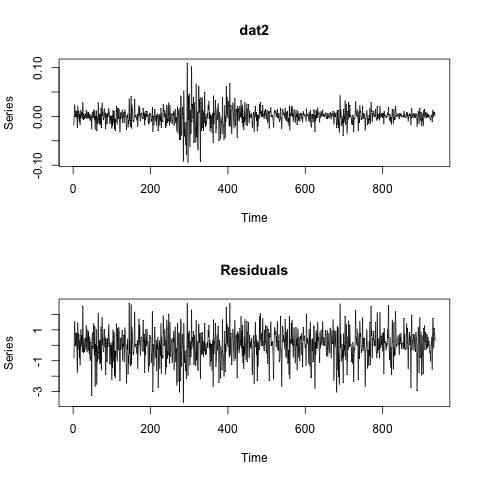
\includegraphics[max size={\textwidth}{\textheight}]{Final_Report_files/Final_Report_43_2.png}
    \par
    \end{center}
    
            \end{InvisibleVerbatim}
            
                \begin{InvisibleVerbatim}
                \vspace{-0.5\baselineskip}
    \begin{center}
    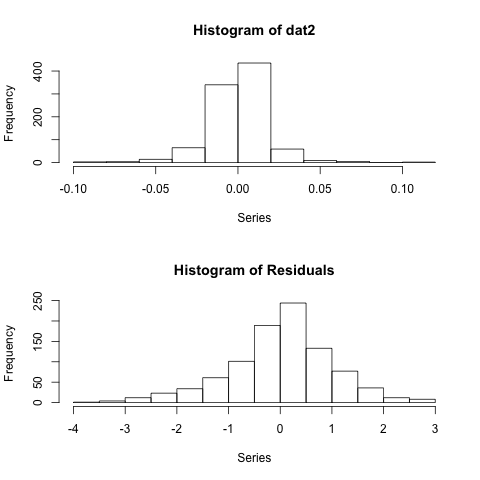
\includegraphics[max size={\textwidth}{\textheight}]{Final_Report_files/Final_Report_43_3.png}
    \par
    \end{center}
    
            \end{InvisibleVerbatim}
            
                \begin{InvisibleVerbatim}
                \vspace{-0.5\baselineskip}
    \begin{center}
    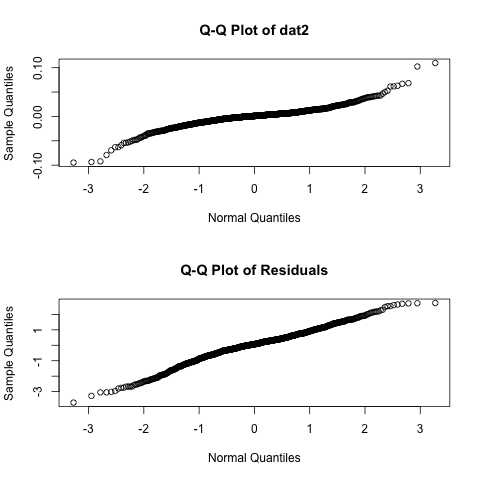
\includegraphics[max size={\textwidth}{\textheight}]{Final_Report_files/Final_Report_43_4.png}
    \par
    \end{center}
    
            \end{InvisibleVerbatim}
            
                \begin{InvisibleVerbatim}
                \vspace{-0.5\baselineskip}
    \begin{center}
    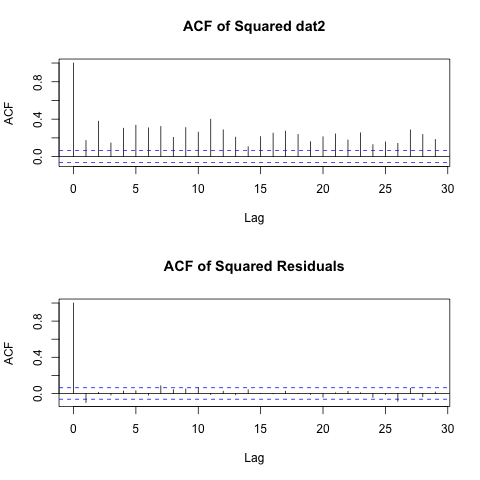
\includegraphics[max size={\textwidth}{\textheight}]{Final_Report_files/Final_Report_43_5.png}
    \par
    \end{center}
    
            \end{InvisibleVerbatim}
            
        
    
\subsection{Log Returns and Residuals}\label{log-returns-and-residuals}Since there're no observable mathematical patterns in the S\&P500 daily
price data, we use the first degree of difference on the price.
i.e.~returns. And then transform it into log returns to distinguish
between series values being uncorrelated and series values being
independent. Because if series values are truly independent from each
other, then nonlinear instantaneous transformations such as taking
logarithms preserves independence. However, those kind of transformation
could alter the characteristic of correlation, as correlation, by its
definition, is only a measure of linear dependence.

The first figures in pre-event and post-event illustrate how log returns
and residuals of S\&P500 daily price evolve through time. As we can see
from the plot log returns give us a more stabilized and a clearer view
of the variance over the time since the plot generally moves around a
horizontal line.

Now we take a closer look to observe the volatility character of the
shown plots. The post event plots exhibit larger fluctuations than the
pre event ones. Also, we observe from the plots of both event that
volatility clustering exists, i.e.~large changes tend to be followed by
large charges and small changes tend to be followed by small changes, of
either sign. This is also a ``stylized fact'' of many economic and
financial variables. In other words, volatility clustering means there
are times stock price is much more volatile than other times. Thus, the
conditional variance of the time series varies over time, that is, there
exists a dynamical pattern in the volatility of a time series.\subsection{Normality of the Data}\label{normality-of-the-data}Since the distributions of log returns and squared residuals of the
two-time periods, as shown in the histogram in the second part of the
figures, are all bell-shaped, the transformed data could be normally
distributed. To test the normality of transformed data. We get the
quatitiles of normal distribution plot through python.\subsection{The Quantiles of Normal Distribution
Plot}\label{the-quantiles-of-normal-distribution-plot}The third part of the figures presents the quantitiles of normal
distribution plots of the data. If the data set is perfectly normal the
points should all fall on the 45 degree y=x line.

The linearity of the pouts suggests the log returns and residuals from
both event are normally distributed. The QQ plot of log returns suggests
that its distribution of post event have a thicker tail than that of a
normal distribution and may be somewhat skewed to the right.\subsection{Autocorrelation Function
Plot}\label{autocorrelation-function-plot}Perform the autocorrelation function on squared log returns. Compare the
plot of autocorrelation function from log returns of pre and post event,
we can see that the ACF values of both event keep falling far out of the
range of two standard deviations away even after long lags, that is the
ACF values are not tailing off gradually. So the time series fit AR
Model. And almost all the ACF values from post event are around or
larger than 0.2 while more than half of ACF values from pre event are
smaller than 0.2.

As for autocorrelation function plot from residuals of pre and post
event, the ACF values of both event fall into the range of two standard
deviations gradually as the lag becomes large, that is the ACF values
tail off gradually. So the time series fit MA Model. And ACF values from
post event are also generally larger than pre event.

The time series from the post event are more autocorrelated than pre
event. The ACF results also collaborate with our point that the
post-event are more volatile than the previous one, i.e.~the effect of
financial crisis is persistent\section{Weekend Effect}\label{weekend-effect}\subsection{Introduction}\label{introduction}

The Weekend Effect is defined as, ``A phenomenon in financial markets in
which stock returns on Mondays are often significantly lower than those
of the immediate preceding Fridays.'' Some theories that explain the
effect attribute the tendency for companies to release bad news on
Friday after the markets close to depressed stock prices on Monday.
However, the others do not acknowledge such weekly tendencies and stated
that it may be a pure stochastic event.

In this module, we intend to employ a series of conventional statistical
methods to analyze whether or not the stock market, resembled by the
SP500 Index, exhibited a tendency against the weekend evenings. Our
intention is to change minds of the traders who believe in the Weekend
Effect.

To begin, we set the workspace, as well as retrive data locally stored
in the work space. Immediately next, we want to split the historical
SP500 data by the days of the week. Hence, append a new column in the
SP500 dataframe, and denote it ``Day.''

    % Make sure that atleast 4 lines are below the HR
    \needspace{4\baselineskip}

    
        \vspace{6pt}
        \makebox[0.1\linewidth]{\smaller\hfill\tt\color{nbframe-in-prompt}In\hspace{4pt}{[}76{]}:\hspace{4pt}}\\*
        \vspace{-2.65\baselineskip}
        \begin{ColorVerbatim}
            \vspace{-0.7\baselineskip}
            \begin{Verbatim}[commandchars=\\\{\}]
\PY{k+kn}{import} \PY{n+nn}{os}
\PY{k}{print} \PY{n}{os}\PY{o}{.}\PY{n}{getcwd}\PY{p}{(}\PY{p}{)}
\PY{n}{os}\PY{o}{.}\PY{n}{chdir}\PY{p}{(}\PY{l+s}{\PYZdq{}}\PY{l+s}{/Users/edwsurewin/Dropbox/Berkeley MA/222/STAT222\PYZhy{}SP500}\PY{l+s}{\PYZdq{}}\PY{p}{)} 
\PY{c}{\PYZsh{} or elsewhere at which \PYZdq{}daily.csv\PYZdq{} is stored}
\end{Verbatim}

            
                \vspace{-0.2\baselineskip}
            
        \end{ColorVerbatim}
    

    

        % If the first block is an image, minipage the image.  Else
        % request a certain amount of space for the input text.
        \needspace{4\baselineskip}
        
        

            % Add document contents.
            
                \begin{InvisibleVerbatim}
                \vspace{-0.5\baselineskip}
\begin{alltt}/Users/edwsurewin/Dropbox/Berkeley MA/222/STAT222-SP500
\end{alltt}

            \end{InvisibleVerbatim}
            
        
    


    % Make sure that atleast 4 lines are below the HR
    \needspace{4\baselineskip}

    
        \vspace{6pt}
        \makebox[0.1\linewidth]{\smaller\hfill\tt\color{nbframe-in-prompt}In\hspace{4pt}{[}77{]}:\hspace{4pt}}\\*
        \vspace{-2.65\baselineskip}
        \begin{ColorVerbatim}
            \vspace{-0.7\baselineskip}
            \begin{Verbatim}[commandchars=\\\{\}]
\PY{k+kn}{import} \PY{n+nn}{pandas} \PY{k+kn}{as} \PY{n+nn}{pd}

\PY{n}{SP500} \PY{o}{=} \PY{n}{pd}\PY{o}{.}\PY{n}{read\PYZus{}csv}\PY{p}{(}\PY{l+s}{\PYZdq{}}\PY{l+s}{daily.csv}\PY{l+s}{\PYZdq{}}\PY{p}{)}
\PY{n}{SP500}\PY{p}{[}\PY{l+s}{\PYZsq{}}\PY{l+s}{Day}\PY{l+s}{\PYZsq{}}\PY{p}{]} \PY{o}{=} \PY{n+nb+bp}{None} \PY{c}{\PYZsh{} create a Day of the Week column}
\PY{k}{print}\PY{p}{(}\PY{n}{SP500}\PY{o}{.}\PY{n}{head}\PY{p}{(}\PY{p}{)}\PY{p}{)}
\end{Verbatim}

            
                \vspace{-0.2\baselineskip}
            
        \end{ColorVerbatim}
    

    

        % If the first block is an image, minipage the image.  Else
        % request a certain amount of space for the input text.
        \needspace{4\baselineskip}
        
        

            % Add document contents.
            
                \begin{InvisibleVerbatim}
                \vspace{-0.5\baselineskip}
\begin{alltt}         Date     Open     High      Low    Close      Volume  Adj
Close   Day
0  2014-02-28  1855.12  1867.92  1847.67  1859.45  3917450000
1859.45  None
1  2014-02-27  1844.90  1854.53  1841.13  1854.29  3547460000
1854.29  None
2  2014-02-26  1845.79  1852.65  1840.66  1845.16  3716730000
1845.16  None
3  2014-02-25  1847.66  1852.91  1840.19  1845.12  3515560000
1845.12  None
4  2014-02-24  1836.78  1858.71  1836.78  1847.61  4014530000
1847.61  None

[5 rows x 8 columns]
\end{alltt}

            \end{InvisibleVerbatim}
            
        
    
\subsection{Quantity of interest}\label{quantity-of-interest}

First of all, we proceed by defining a quantity of interest. Since we
are interested in the overnight changes, we are interested in the
overnight returns by days of the week. Denote overnight return
$R_{today}= \frac{Next-Trading-Day-Opening}{Today's-Adjusted-Close}$.Therefore, during any given ordinary week without holidays
(i.e.~non-trading days), we have five overnight returns. Next, we
defined a function that automates computing the rate of return for any
two consecutive trading days. Then, we employed a built-in package in
python, which calculates the ``day of the week'' indicator for each row
observation.

Once we had the returns computed together with the indicators, we
construct five dynamic lists to store Monday, Tuesday, Wednesday,
Thursday, and Friday overnight returns, respectively.

    % Make sure that atleast 4 lines are below the HR
    \needspace{4\baselineskip}

    
        \vspace{6pt}
        \makebox[0.1\linewidth]{\smaller\hfill\tt\color{nbframe-in-prompt}In\hspace{4pt}{[}78{]}:\hspace{4pt}}\\*
        \vspace{-2.65\baselineskip}
        \begin{ColorVerbatim}
            \vspace{-0.7\baselineskip}
            \begin{Verbatim}[commandchars=\\\{\}]
\PY{c}{\PYZsh{} print(SP500.tail()) = 0 to 16146}
\PY{c}{\PYZsh{} len(SP500[\PYZsq{}Day\PYZsq{}]) = 16147`}

\PY{n}{rate} \PY{o}{=} \PY{p}{[}\PY{n+nb+bp}{None}\PY{p}{]}\PY{o}{*}\PY{p}{(}\PY{n+nb}{len}\PY{p}{(}\PY{n}{SP500}\PY{p}{[}\PY{l+s}{\PYZsq{}}\PY{l+s}{Day}\PY{l+s}{\PYZsq{}}\PY{p}{]}\PY{p}{)}\PY{o}{\PYZhy{}}\PY{l+m+mi}{1}\PY{p}{)}

\PY{c}{\PYZsh{}create an array and fill in }
\PY{k}{def} \PY{n+nf}{compute\PYZus{}rate}\PY{p}{(}\PY{n}{SP500}\PY{p}{,} \PY{n}{rate}\PY{p}{)}\PY{p}{:}
    \PY{k}{for} \PY{n}{i} \PY{o+ow}{in} \PY{n+nb}{range}\PY{p}{(}\PY{l+m+mi}{0}\PY{p}{,} \PY{n+nb}{len}\PY{p}{(}\PY{n}{SP500}\PY{p}{[}\PY{l+s}{\PYZsq{}}\PY{l+s}{Day}\PY{l+s}{\PYZsq{}}\PY{p}{]}\PY{p}{)}\PY{o}{\PYZhy{}}\PY{l+m+mi}{1}\PY{p}{)}\PY{p}{:}
        \PY{n}{rate}\PY{p}{[}\PY{n}{i}\PY{p}{]} \PY{o}{=} \PY{n}{SP500}\PY{p}{[}\PY{l+s}{\PYZsq{}}\PY{l+s}{Open}\PY{l+s}{\PYZsq{}}\PY{p}{]}\PY{p}{[}\PY{n}{i}\PY{p}{]}\PY{o}{/}\PY{n}{SP500}\PY{p}{[}\PY{l+s}{\PYZsq{}}\PY{l+s}{Adj Close}\PY{l+s}{\PYZsq{}}\PY{p}{]}\PY{p}{[}\PY{n}{i}\PY{o}{+}\PY{l+m+mi}{1}\PY{p}{]}
    \PY{k}{return} \PY{n}{rate}

\PY{n}{rate} \PY{o}{=} \PY{n}{compute\PYZus{}rate}\PY{p}{(}\PY{n}{SP500}\PY{p}{,} \PY{n}{rate}\PY{p}{)}

\PY{c}{\PYZsh{} first 5 items in open/close rate list}
\PY{k}{print}\PY{p}{(}\PY{n}{rate}\PY{p}{[}\PY{l+m+mi}{0}\PY{p}{:}\PY{l+m+mi}{5}\PY{p}{]}\PY{p}{)} 
\end{Verbatim}

            
                \vspace{-0.2\baselineskip}
            
        \end{ColorVerbatim}
    

    

        % If the first block is an image, minipage the image.  Else
        % request a certain amount of space for the input text.
        \needspace{4\baselineskip}
        
        

            % Add document contents.
            
                \begin{InvisibleVerbatim}
                \vspace{-0.5\baselineskip}
\begin{alltt}[1.0004476106757842, 0.99985909081055302, 1.0003631200138745,
1.0000270619881904, 1.0002886317222601]
\end{alltt}

            \end{InvisibleVerbatim}
            
        
    


    % Make sure that atleast 4 lines are below the HR
    \needspace{4\baselineskip}

    
        \vspace{6pt}
        \makebox[0.1\linewidth]{\smaller\hfill\tt\color{nbframe-in-prompt}In\hspace{4pt}{[}79{]}:\hspace{4pt}}\\*
        \vspace{-2.65\baselineskip}
        \begin{ColorVerbatim}
            \vspace{-0.7\baselineskip}
            \begin{Verbatim}[commandchars=\\\{\}]
\PY{k+kn}{import} \PY{n+nn}{datetime}

\PY{c}{\PYZsh{} fill out the days of the weeks}
\PY{c}{\PYZsh{} 1: Monday, 2: Tuesday, ..., 5: Friday}

\PY{k}{for} \PY{n}{i} \PY{o+ow}{in} \PY{n+nb}{range}\PY{p}{(}\PY{l+m+mi}{0}\PY{p}{,} \PY{n+nb}{len}\PY{p}{(}\PY{n}{SP500}\PY{p}{[}\PY{l+s}{\PYZsq{}}\PY{l+s}{Day}\PY{l+s}{\PYZsq{}}\PY{p}{]}\PY{p}{)}\PY{p}{)}\PY{p}{:}   
    \PY{n}{SP500}\PY{p}{[}\PY{l+s}{\PYZsq{}}\PY{l+s}{Day}\PY{l+s}{\PYZsq{}}\PY{p}{]}\PY{p}{[}\PY{n}{i}\PY{p}{]} \PY{o}{=} \PY{n}{datetime}\PY{o}{.}\PY{n}{date}\PY{p}{(}\PY{n+nb}{int}\PY{p}{(}\PY{n}{SP500}\PY{p}{[}\PY{l+s}{\PYZsq{}}\PY{l+s}{Date}\PY{l+s}{\PYZsq{}}\PY{p}{]}\PY{p}{[}\PY{n}{i}\PY{p}{]}\PY{p}{[}\PY{l+m+mi}{0}\PY{p}{:}\PY{l+m+mi}{4}\PY{p}{]}\PY{p}{)}\PY{p}{,} \PY{n+nb}{int}\PY{p}{(}\PY{n}{SP500}\PY{p}{[}\PY{l+s}{\PYZsq{}}\PY{l+s}{Date}\PY{l+s}{\PYZsq{}}\PY{p}{]}\PY{p}{[}\PY{n}{i}\PY{p}{]}\PY{p}{[}\PY{l+m+mi}{5}\PY{p}{:}\PY{l+m+mi}{7}\PY{p}{]}\PY{p}{)}\PY{p}{,} \PY{n+nb}{int}\PY{p}{(}\PY{n}{SP500}\PY{p}{[}\PY{l+s}{\PYZsq{}}\PY{l+s}{Date}\PY{l+s}{\PYZsq{}}\PY{p}{]}\PY{p}{[}\PY{n}{i}\PY{p}{]}\PY{p}{[}\PY{l+m+mi}{8}\PY{p}{:}\PY{l+m+mi}{10}\PY{p}{]}\PY{p}{)}\PY{p}{)}\PY{o}{.}\PY{n}{isoweekday}\PY{p}{(}\PY{p}{)}

\PY{k}{print}\PY{p}{(}\PY{n}{SP500}\PY{o}{.}\PY{n}{head}\PY{p}{(}\PY{p}{)}\PY{p}{)}
\end{Verbatim}

            
                \vspace{-0.2\baselineskip}
            
        \end{ColorVerbatim}
    

    

        % If the first block is an image, minipage the image.  Else
        % request a certain amount of space for the input text.
        \needspace{4\baselineskip}
        
        

            % Add document contents.
            
                \begin{InvisibleVerbatim}
                \vspace{-0.5\baselineskip}
\begin{alltt}         Date     Open     High      Low    Close      Volume  Adj
Close Day
0  2014-02-28  1855.12  1867.92  1847.67  1859.45  3917450000
1859.45   5
1  2014-02-27  1844.90  1854.53  1841.13  1854.29  3547460000
1854.29   4
2  2014-02-26  1845.79  1852.65  1840.66  1845.16  3716730000
1845.16   3
3  2014-02-25  1847.66  1852.91  1840.19  1845.12  3515560000
1845.12   2
4  2014-02-24  1836.78  1858.71  1836.78  1847.61  4014530000
1847.61   1

[5 rows x 8 columns]
\end{alltt}

            \end{InvisibleVerbatim}
            
        
    


    % Make sure that atleast 4 lines are below the HR
    \needspace{4\baselineskip}

    
        \vspace{6pt}
        \makebox[0.1\linewidth]{\smaller\hfill\tt\color{nbframe-in-prompt}In\hspace{4pt}{[}80{]}:\hspace{4pt}}\\*
        \vspace{-2.65\baselineskip}
        \begin{ColorVerbatim}
            \vspace{-0.7\baselineskip}
            \begin{Verbatim}[commandchars=\\\{\}]
\PY{c}{\PYZsh{} create dynamic lists to store overnight returns of corresponding days of the week}
\PY{c}{\PYZsh{} control group  Friday, whereas experiment group  any other day(s) of the week}

\PY{c}{\PYZsh{} e.g. a Monday\PYZsq{}s overnight is defined to be }
\PY{c}{\PYZsh{}      (the quotient of) Tuesday Opening / Monday\PYZsq{}s Adj Close}

\PY{n}{Monday} \PY{o}{=} \PY{p}{[}\PY{p}{]}       
\PY{n}{Tuesday} \PY{o}{=} \PY{p}{[}\PY{p}{]}      
\PY{n}{Wednesday} \PY{o}{=} \PY{p}{[}\PY{p}{]}    
\PY{n}{Thursday} \PY{o}{=} \PY{p}{[}\PY{p}{]}     
\PY{n}{Friday} \PY{o}{=} \PY{p}{[}\PY{p}{]}       

\PY{k}{for} \PY{n}{i} \PY{o+ow}{in} \PY{n+nb}{range}\PY{p}{(}\PY{l+m+mi}{1}\PY{p}{,} \PY{n+nb}{len}\PY{p}{(}\PY{n}{SP500}\PY{p}{[}\PY{l+s}{\PYZsq{}}\PY{l+s}{Day}\PY{l+s}{\PYZsq{}}\PY{p}{]}\PY{p}{)}\PY{p}{)}\PY{p}{:}
    \PY{k}{if} \PY{n}{SP500}\PY{p}{[}\PY{l+s}{\PYZsq{}}\PY{l+s}{Day}\PY{l+s}{\PYZsq{}}\PY{p}{]}\PY{p}{[}\PY{n}{i}\PY{p}{]} \PY{o}{==} \PY{l+m+mi}{1}\PY{p}{:}
        \PY{n}{Monday}\PY{o}{.}\PY{n}{append}\PY{p}{(}\PY{n}{rate}\PY{p}{[}\PY{n}{i}\PY{o}{\PYZhy{}}\PY{l+m+mi}{1}\PY{p}{]}\PY{p}{)}
    \PY{k}{else}\PY{p}{:}
        \PY{k}{if} \PY{n}{SP500}\PY{p}{[}\PY{l+s}{\PYZsq{}}\PY{l+s}{Day}\PY{l+s}{\PYZsq{}}\PY{p}{]}\PY{p}{[}\PY{n}{i}\PY{p}{]} \PY{o}{==} \PY{l+m+mi}{2}\PY{p}{:}
            \PY{n}{Tuesday}\PY{o}{.}\PY{n}{append}\PY{p}{(}\PY{n}{rate}\PY{p}{[}\PY{n}{i}\PY{o}{\PYZhy{}}\PY{l+m+mi}{1}\PY{p}{]}\PY{p}{)}
        \PY{k}{else}\PY{p}{:}
            \PY{k}{if} \PY{n}{SP500}\PY{p}{[}\PY{l+s}{\PYZsq{}}\PY{l+s}{Day}\PY{l+s}{\PYZsq{}}\PY{p}{]}\PY{p}{[}\PY{n}{i}\PY{p}{]} \PY{o}{==} \PY{l+m+mi}{3}\PY{p}{:}
                \PY{n}{Wednesday}\PY{o}{.}\PY{n}{append}\PY{p}{(}\PY{n}{rate}\PY{p}{[}\PY{n}{i}\PY{o}{\PYZhy{}}\PY{l+m+mi}{1}\PY{p}{]}\PY{p}{)}
            \PY{k}{else}\PY{p}{:}
                \PY{k}{if} \PY{n}{SP500}\PY{p}{[}\PY{l+s}{\PYZsq{}}\PY{l+s}{Day}\PY{l+s}{\PYZsq{}}\PY{p}{]}\PY{p}{[}\PY{n}{i}\PY{p}{]} \PY{o}{==} \PY{l+m+mi}{4}\PY{p}{:}
                    \PY{n}{Thursday}\PY{o}{.}\PY{n}{append}\PY{p}{(}\PY{n}{rate}\PY{p}{[}\PY{n}{i}\PY{o}{\PYZhy{}}\PY{l+m+mi}{1}\PY{p}{]}\PY{p}{)}
                \PY{k}{else}\PY{p}{:}
                    \PY{k}{if} \PY{n}{SP500}\PY{p}{[}\PY{l+s}{\PYZsq{}}\PY{l+s}{Day}\PY{l+s}{\PYZsq{}}\PY{p}{]}\PY{p}{[}\PY{n}{i}\PY{p}{]} \PY{o}{==} \PY{l+m+mi}{5}\PY{p}{:}
                        \PY{n}{Friday}\PY{o}{.}\PY{n}{append}\PY{p}{(}\PY{n}{rate}\PY{p}{[}\PY{n}{i}\PY{o}{\PYZhy{}}\PY{l+m+mi}{1}\PY{p}{]}\PY{p}{)}   
\PY{c}{\PYZsh{} recent 10 years}
\PY{n}{Monday} \PY{o}{=} \PY{n}{Monday}\PY{p}{[}\PY{l+m+mi}{0}\PY{p}{:}\PY{l+m+mi}{520}\PY{p}{]}      
\PY{n}{Tuesday} \PY{o}{=} \PY{n}{Tuesday}\PY{p}{[}\PY{l+m+mi}{0}\PY{p}{:}\PY{l+m+mi}{520}\PY{p}{]}      
\PY{n}{Wednesday} \PY{o}{=} \PY{n}{Wednesday}\PY{p}{[}\PY{l+m+mi}{0}\PY{p}{:}\PY{l+m+mi}{520}\PY{p}{]}     
\PY{n}{Thursday} \PY{o}{=} \PY{n}{Thursday}\PY{p}{[}\PY{l+m+mi}{0}\PY{p}{:}\PY{l+m+mi}{520}\PY{p}{]}       
\PY{n}{Friday} \PY{o}{=} \PY{n}{Friday}\PY{p}{[}\PY{l+m+mi}{0}\PY{p}{:}\PY{l+m+mi}{520}\PY{p}{]}     
                
\PY{c}{\PYZsh{} for exmaple, Friday vs. NonFriday}
\PY{n}{NonFri} \PY{o}{=} \PY{n}{Monday} \PY{o}{+} \PY{n}{Tuesday} \PY{o}{+} \PY{n}{Wednesday} \PY{o}{+} \PY{n}{Thursday}
\end{Verbatim}

            
                \vspace{-0.2\baselineskip}
            
        \end{ColorVerbatim}
    
\subsection{Quantity of Interest
Plots}\label{quantity-of-interest-plots}

Before moving on, we subset the first 520 elements in each list;
therefore, we have roughly the recent 10-year data to analyze upon. The
reason of subsetting is that the fundamentals of stock market might have
changed substantially over the last decades, and historical data from
the past could tell little about the current dynamics in today's market.
We want to rule out the noises due to a different financial regulation
settings happenend in the past, and want to solely pinpoint what's
happened recently.

With the data cleaned and sort, we would like to have a visual
impression how the data look like, and whether we could draw any
immediate preliminary conclusion from the pictures. We plotted the
following 4 pictures, with each of the Friday group and another day of
the week. Notice that the Friday group is the control group, and 4 other
groups are the treatment groups; in other words, we apply another day of
the week and try to observe possiblity of significance improvements.

On the x-axis, we have ``chronological number of weeks until March 6th,
2014'', when we lastly accessed the public data from Yahoo Faince. On
the y-axis, we have the quantitiy of interest being plotted, i.e.~the
overnight rates of return. The red dots are of the Friday group, the
black dots are of the respective treatement groups. We attempt to answer
these questions:

\begin{enumerate}
\def\labelenumi{\arabic{enumi})}
\itemsep1pt\parskip0pt\parsep0pt
\item
  Are all the red dots systematically lower than the black dots?
\item
  If so, which picture shows the most apparent difference?
\item
  Any patterns?
\end{enumerate}

To answer these questions, we take a closer look at each picture. It
seems that the answers for the first two questions are negative, while
we can say something about the 3). It appears that we experienced a
period of volatilities during Week 100 to Week 300; if we convert the
dates back to calendar, we will notice that that was the period we were
in the financial meltdown commercing 2007. Hence, the pictures
nevertheless showed we caputured the data correctly.

Yet, we are not able to make any statements with regards to the research
objective.

    % Make sure that atleast 4 lines are below the HR
    \needspace{4\baselineskip}

    
        \vspace{6pt}
        \makebox[0.1\linewidth]{\smaller\hfill\tt\color{nbframe-in-prompt}In\hspace{4pt}{[}81{]}:\hspace{4pt}}\\*
        \vspace{-2.65\baselineskip}
        \begin{ColorVerbatim}
            \vspace{-0.7\baselineskip}
            \begin{Verbatim}[commandchars=\\\{\}]
\PY{k+kn}{import} \PY{n+nn}{numpy}
\PY{k+kn}{import} \PY{n+nn}{matplotlib}

\PY{c}{\PYZsh{} overnight return: Monday vs. Friday}
\PY{c}{\PYZsh{} X\PYZhy{}axis is timeline in chronological order}

\PY{n}{plt}\PY{o}{.}\PY{n}{plot}\PY{p}{(}\PY{n}{Monday}\PY{p}{,} \PY{l+s}{\PYZsq{}}\PY{l+s}{ko}\PY{l+s}{\PYZsq{}}\PY{p}{,} \PY{n}{label}\PY{o}{=}\PY{l+s}{\PYZsq{}}\PY{l+s}{Monday}\PY{l+s}{\PYZsq{}}\PY{p}{)}
\PY{n}{plt}\PY{o}{.}\PY{n}{hold}\PY{p}{(}\PY{n+nb+bp}{True}\PY{p}{)}
\PY{n}{plt}\PY{o}{.}\PY{n}{plot}\PY{p}{(}\PY{n}{Friday}\PY{p}{,} \PY{l+s}{\PYZsq{}}\PY{l+s}{ro}\PY{l+s}{\PYZsq{}}\PY{p}{,} \PY{n}{label}\PY{o}{=}\PY{l+s}{\PYZsq{}}\PY{l+s}{Friday}\PY{l+s}{\PYZsq{}}\PY{p}{,} \PY{n}{alpha}\PY{o}{=}\PY{l+m+mf}{0.7}\PY{p}{)}
\PY{n}{plt}\PY{o}{.}\PY{n}{legend}\PY{p}{(}\PY{n}{loc}\PY{o}{=}\PY{l+m+mi}{0}\PY{p}{)}
\PY{n}{plt}\PY{o}{.}\PY{n}{title}\PY{p}{(}\PY{l+s}{\PYZsq{}}\PY{l+s}{Overnight Return Comparison, Fri vs. Mon}\PY{l+s}{\PYZsq{}}\PY{p}{)}
\PY{n}{plt}\PY{o}{.}\PY{n}{ylabel}\PY{p}{(}\PY{l+s}{\PYZsq{}}\PY{l+s}{Overnight Return}\PY{l+s}{\PYZsq{}}\PY{p}{)}
\PY{n}{plt}\PY{o}{.}\PY{n}{xlabel}\PY{p}{(}\PY{l+s}{\PYZsq{}}\PY{l+s}{Chronological \PYZsh{} of Weeks until Mar 06 2014}\PY{l+s}{\PYZsq{}}\PY{p}{)}
\end{Verbatim}

            
                \vspace{-0.2\baselineskip}
            
        \end{ColorVerbatim}
    

    

        % If the first block is an image, minipage the image.  Else
        % request a certain amount of space for the input text.
        \needspace{4\baselineskip}
        
        

            % Add document contents.
            
                \makebox[0.1\linewidth]{\smaller\hfill\tt\color{nbframe-out-prompt}Out\hspace{4pt}{[}81{]}:\hspace{4pt}}\\*
                \vspace{-2.55\baselineskip}\begin{InvisibleVerbatim}
                \vspace{-0.5\baselineskip}
\begin{alltt}<matplotlib.text.Text at 0x1125562d0>\end{alltt}

            \end{InvisibleVerbatim}
            
                \begin{InvisibleVerbatim}
                \vspace{-0.5\baselineskip}
    \begin{center}
    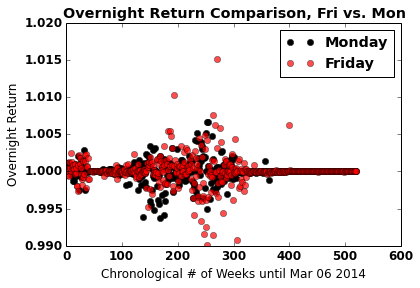
\includegraphics[max size={\textwidth}{\textheight}]{Final_Report_files/Final_Report_62_1.png}
    \par
    \end{center}
    
            \end{InvisibleVerbatim}
            
        
    


    % Make sure that atleast 4 lines are below the HR
    \needspace{4\baselineskip}

    
        \vspace{6pt}
        \makebox[0.1\linewidth]{\smaller\hfill\tt\color{nbframe-in-prompt}In\hspace{4pt}{[}82{]}:\hspace{4pt}}\\*
        \vspace{-2.65\baselineskip}
        \begin{ColorVerbatim}
            \vspace{-0.7\baselineskip}
            \begin{Verbatim}[commandchars=\\\{\}]
\PY{c}{\PYZsh{} overnight return: Tuesday vs. Friday}
\PY{c}{\PYZsh{} X\PYZhy{}axis is timeline in chronological order}

\PY{n}{plt}\PY{o}{.}\PY{n}{plot}\PY{p}{(}\PY{n}{Tuesday}\PY{p}{,} \PY{l+s}{\PYZsq{}}\PY{l+s}{ko}\PY{l+s}{\PYZsq{}}\PY{p}{,} \PY{n}{label}\PY{o}{=}\PY{l+s}{\PYZsq{}}\PY{l+s}{Tuesday}\PY{l+s}{\PYZsq{}}\PY{p}{)}
\PY{n}{plt}\PY{o}{.}\PY{n}{hold}\PY{p}{(}\PY{n+nb+bp}{True}\PY{p}{)}
\PY{n}{plt}\PY{o}{.}\PY{n}{plot}\PY{p}{(}\PY{n}{Friday}\PY{p}{,} \PY{l+s}{\PYZsq{}}\PY{l+s}{ro}\PY{l+s}{\PYZsq{}}\PY{p}{,} \PY{n}{label}\PY{o}{=}\PY{l+s}{\PYZsq{}}\PY{l+s}{Friday}\PY{l+s}{\PYZsq{}}\PY{p}{,} \PY{n}{alpha}\PY{o}{=}\PY{l+m+mf}{0.7}\PY{p}{)}
\PY{n}{plt}\PY{o}{.}\PY{n}{title}\PY{p}{(}\PY{l+s}{\PYZsq{}}\PY{l+s}{Overnight Return Comparison, Fri vs. Tue}\PY{l+s}{\PYZsq{}}\PY{p}{)}
\PY{n}{plt}\PY{o}{.}\PY{n}{ylabel}\PY{p}{(}\PY{l+s}{\PYZsq{}}\PY{l+s}{Overnight Return}\PY{l+s}{\PYZsq{}}\PY{p}{)}
\PY{n}{plt}\PY{o}{.}\PY{n}{xlabel}\PY{p}{(}\PY{l+s}{\PYZsq{}}\PY{l+s}{Chronological \PYZsh{} of Weeks until Mar 06 2014}\PY{l+s}{\PYZsq{}}\PY{p}{)}
\PY{n}{plt}\PY{o}{.}\PY{n}{legend}\PY{p}{(}\PY{n}{loc}\PY{o}{=}\PY{l+m+mi}{0}\PY{p}{)}
\end{Verbatim}

            
                \vspace{-0.2\baselineskip}
            
        \end{ColorVerbatim}
    

    

        % If the first block is an image, minipage the image.  Else
        % request a certain amount of space for the input text.
        \needspace{4\baselineskip}
        
        

            % Add document contents.
            
                \makebox[0.1\linewidth]{\smaller\hfill\tt\color{nbframe-out-prompt}Out\hspace{4pt}{[}82{]}:\hspace{4pt}}\\*
                \vspace{-2.55\baselineskip}\begin{InvisibleVerbatim}
                \vspace{-0.5\baselineskip}
\begin{alltt}<matplotlib.legend.Legend at 0x10e0c3f10>\end{alltt}

            \end{InvisibleVerbatim}
            
                \begin{InvisibleVerbatim}
                \vspace{-0.5\baselineskip}
    \begin{center}
    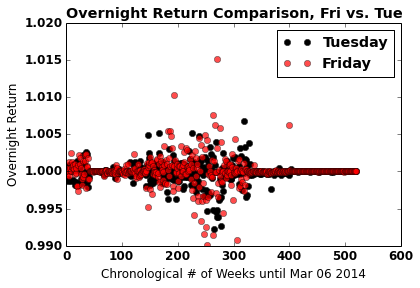
\includegraphics[max size={\textwidth}{\textheight}]{Final_Report_files/Final_Report_63_1.png}
    \par
    \end{center}
    
            \end{InvisibleVerbatim}
            
        
    


    % Make sure that atleast 4 lines are below the HR
    \needspace{4\baselineskip}

    
        \vspace{6pt}
        \makebox[0.1\linewidth]{\smaller\hfill\tt\color{nbframe-in-prompt}In\hspace{4pt}{[}83{]}:\hspace{4pt}}\\*
        \vspace{-2.65\baselineskip}
        \begin{ColorVerbatim}
            \vspace{-0.7\baselineskip}
            \begin{Verbatim}[commandchars=\\\{\}]
\PY{c}{\PYZsh{} overnight return: Wednesday vs. Friday}
\PY{c}{\PYZsh{} X\PYZhy{}axis is timeline in chronological order}

\PY{n}{plt}\PY{o}{.}\PY{n}{plot}\PY{p}{(}\PY{n}{Wednesday}\PY{p}{,} \PY{l+s}{\PYZsq{}}\PY{l+s}{ko}\PY{l+s}{\PYZsq{}}\PY{p}{,} \PY{n}{label}\PY{o}{=}\PY{l+s}{\PYZsq{}}\PY{l+s}{Wednesday}\PY{l+s}{\PYZsq{}}\PY{p}{)}
\PY{n}{plt}\PY{o}{.}\PY{n}{hold}\PY{p}{(}\PY{n+nb+bp}{True}\PY{p}{)}
\PY{n}{plt}\PY{o}{.}\PY{n}{plot}\PY{p}{(}\PY{n}{Friday}\PY{p}{,} \PY{l+s}{\PYZsq{}}\PY{l+s}{ro}\PY{l+s}{\PYZsq{}}\PY{p}{,} \PY{n}{label}\PY{o}{=}\PY{l+s}{\PYZsq{}}\PY{l+s}{Friday}\PY{l+s}{\PYZsq{}}\PY{p}{,} \PY{n}{alpha}\PY{o}{=}\PY{l+m+mf}{0.7}\PY{p}{)}
\PY{n}{plt}\PY{o}{.}\PY{n}{title}\PY{p}{(}\PY{l+s}{\PYZsq{}}\PY{l+s}{Overnight Return Comparison, Fri vs. Wed}\PY{l+s}{\PYZsq{}}\PY{p}{)}
\PY{n}{plt}\PY{o}{.}\PY{n}{ylabel}\PY{p}{(}\PY{l+s}{\PYZsq{}}\PY{l+s}{Overnight Return}\PY{l+s}{\PYZsq{}}\PY{p}{)}
\PY{n}{plt}\PY{o}{.}\PY{n}{xlabel}\PY{p}{(}\PY{l+s}{\PYZsq{}}\PY{l+s}{Chronological \PYZsh{} of Weeks until Mar 06 2014}\PY{l+s}{\PYZsq{}}\PY{p}{)}
\PY{n}{plt}\PY{o}{.}\PY{n}{legend}\PY{p}{(}\PY{n}{loc}\PY{o}{=}\PY{l+m+mi}{0}\PY{p}{)}
\end{Verbatim}

            
                \vspace{-0.2\baselineskip}
            
        \end{ColorVerbatim}
    

    

        % If the first block is an image, minipage the image.  Else
        % request a certain amount of space for the input text.
        \needspace{4\baselineskip}
        
        

            % Add document contents.
            
                \makebox[0.1\linewidth]{\smaller\hfill\tt\color{nbframe-out-prompt}Out\hspace{4pt}{[}83{]}:\hspace{4pt}}\\*
                \vspace{-2.55\baselineskip}\begin{InvisibleVerbatim}
                \vspace{-0.5\baselineskip}
\begin{alltt}<matplotlib.legend.Legend at 0x10e0fd3d0>\end{alltt}

            \end{InvisibleVerbatim}
            
                \begin{InvisibleVerbatim}
                \vspace{-0.5\baselineskip}
    \begin{center}
    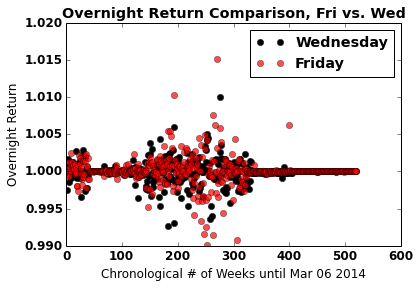
\includegraphics[max size={\textwidth}{\textheight}]{Final_Report_files/Final_Report_64_1.png}
    \par
    \end{center}
    
            \end{InvisibleVerbatim}
            
        
    


    % Make sure that atleast 4 lines are below the HR
    \needspace{4\baselineskip}

    
        \vspace{6pt}
        \makebox[0.1\linewidth]{\smaller\hfill\tt\color{nbframe-in-prompt}In\hspace{4pt}{[}84{]}:\hspace{4pt}}\\*
        \vspace{-2.65\baselineskip}
        \begin{ColorVerbatim}
            \vspace{-0.7\baselineskip}
            \begin{Verbatim}[commandchars=\\\{\}]
\PY{c}{\PYZsh{} overnight return: Thursday vs. Friday}
\PY{c}{\PYZsh{} X\PYZhy{}axis is timeline in chronological order}

\PY{n}{plt}\PY{o}{.}\PY{n}{plot}\PY{p}{(}\PY{n}{Thursday}\PY{p}{,} \PY{l+s}{\PYZsq{}}\PY{l+s}{ko}\PY{l+s}{\PYZsq{}}\PY{p}{,} \PY{n}{label}\PY{o}{=}\PY{l+s}{\PYZsq{}}\PY{l+s}{Thursday}\PY{l+s}{\PYZsq{}}\PY{p}{)}
\PY{n}{plt}\PY{o}{.}\PY{n}{hold}\PY{p}{(}\PY{n+nb+bp}{True}\PY{p}{)}
\PY{n}{plt}\PY{o}{.}\PY{n}{plot}\PY{p}{(}\PY{n}{Friday}\PY{p}{,} \PY{l+s}{\PYZsq{}}\PY{l+s}{ro}\PY{l+s}{\PYZsq{}}\PY{p}{,} \PY{n}{label}\PY{o}{=}\PY{l+s}{\PYZsq{}}\PY{l+s}{Friday}\PY{l+s}{\PYZsq{}}\PY{p}{,} \PY{n}{alpha}\PY{o}{=}\PY{l+m+mf}{0.7}\PY{p}{)}
\PY{n}{plt}\PY{o}{.}\PY{n}{title}\PY{p}{(}\PY{l+s}{\PYZsq{}}\PY{l+s}{Overnight Return Comparison, Fri vs. Thurs}\PY{l+s}{\PYZsq{}}\PY{p}{)}
\PY{n}{plt}\PY{o}{.}\PY{n}{ylabel}\PY{p}{(}\PY{l+s}{\PYZsq{}}\PY{l+s}{Overnight Return}\PY{l+s}{\PYZsq{}}\PY{p}{)}
\PY{n}{plt}\PY{o}{.}\PY{n}{xlabel}\PY{p}{(}\PY{l+s}{\PYZsq{}}\PY{l+s}{Chronological \PYZsh{} of Weeks until Mar 06 2014}\PY{l+s}{\PYZsq{}}\PY{p}{)}
\PY{n}{plt}\PY{o}{.}\PY{n}{legend}\PY{p}{(}\PY{n}{loc}\PY{o}{=}\PY{l+m+mi}{0}\PY{p}{)}
\end{Verbatim}

            
                \vspace{-0.2\baselineskip}
            
        \end{ColorVerbatim}
    

    

        % If the first block is an image, minipage the image.  Else
        % request a certain amount of space for the input text.
        \needspace{4\baselineskip}
        
        

            % Add document contents.
            
                \makebox[0.1\linewidth]{\smaller\hfill\tt\color{nbframe-out-prompt}Out\hspace{4pt}{[}84{]}:\hspace{4pt}}\\*
                \vspace{-2.55\baselineskip}\begin{InvisibleVerbatim}
                \vspace{-0.5\baselineskip}
\begin{alltt}<matplotlib.legend.Legend at 0x10e0b2910>\end{alltt}

            \end{InvisibleVerbatim}
            
                \begin{InvisibleVerbatim}
                \vspace{-0.5\baselineskip}
    \begin{center}
    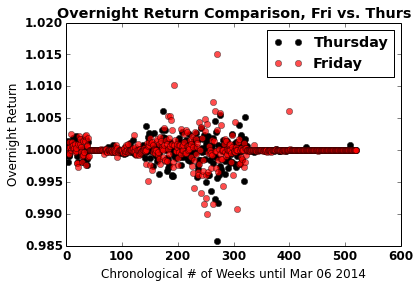
\includegraphics[max size={\textwidth}{\textheight}]{Final_Report_files/Final_Report_65_1.png}
    \par
    \end{center}
    
            \end{InvisibleVerbatim}
            
        
    
Naturally, we are going to empower our research by performing a series
of statistical tests, wherever applicable. Notice that most tests have a
distinct set of requirements under which the data have to suffice. For
the time being, we are willing to assume all required, although that
could lead us to an aggressive concludsion.\subsection{Mann--Whitney U Test}\label{mannwhitney-u-test}

More efficient than the T test in non-normal distribution, this test is
said to embrace a very general formulation which assumes that:

\begin{enumerate}
\def\labelenumi{\arabic{enumi}.}
\itemsep1pt\parskip0pt\parsep0pt
\item
  All the observations from both groups are independent of each other,
\item
  The responses are ordinal (i.e.~one can at least say, of any two
  observations, which is the greater),
\item
  The distributions of both groups are equal under the null hypothesis,
  so that the probability of an observation from one population (X)
  exceeding an observation from the second population (Y) equals the
  probability of an observation from Y exceeding an observation from X.
  That is, there is a symmetry between populations with respect to
  probability of random drawing of a larger observation.
\item
  Under the alternative hypothesis, the probability of an observation
  from one population (X) exceeding an observation from the second
  population (Y) (after exclusion of ties) is not equal to 0.5. The
  alternative may also be stated in terms of a one-sided test, for
  example: P(X~\textgreater{}~Y)~+~0.5 P(X~=~Y) ~is greater than~0.5.
\end{enumerate}

Thus, null is mean(Friday) = mean(nonFriday), and inequality otherwise.

    % Make sure that atleast 4 lines are below the HR
    \needspace{4\baselineskip}

    
        \vspace{6pt}
        \makebox[0.1\linewidth]{\smaller\hfill\tt\color{nbframe-in-prompt}In\hspace{4pt}{[}85{]}:\hspace{4pt}}\\*
        \vspace{-2.65\baselineskip}
        \begin{ColorVerbatim}
            \vspace{-0.7\baselineskip}
            \begin{Verbatim}[commandchars=\\\{\}]
\PY{k+kn}{import} \PY{n+nn}{scipy.stats} \PY{k+kn}{as} \PY{n+nn}{stats}
\PY{n}{u}\PY{p}{,} \PY{n}{MW\PYZus{}p\PYZus{}value} \PY{o}{=} \PY{n}{stats}\PY{o}{.}\PY{n}{mannwhitneyu}\PY{p}{(}\PY{n}{Friday}\PY{p}{,} \PY{n}{NonFri}\PY{p}{)}
\PY{k}{print}\PY{p}{(}\PY{l+s}{\PYZdq{}}\PY{l+s}{two\PYZhy{}sample wilcoxon\PYZhy{}test p\PYZhy{}value is}\PY{l+s}{\PYZdq{}}\PY{p}{,} \PY{n}{MW\PYZus{}p\PYZus{}value}\PY{p}{)}

\PY{c}{\PYZsh{} p\PYZus{}value \PYZlt{} 0.01 =\PYZgt{} alternative hypothesis:}
\PY{c}{\PYZsh{} they don\PYZsq{}t have the same mean at the 1\PYZpc{} significance level}
\end{Verbatim}

            
                \vspace{-0.2\baselineskip}
            
        \end{ColorVerbatim}
    

    

        % If the first block is an image, minipage the image.  Else
        % request a certain amount of space for the input text.
        \needspace{4\baselineskip}
        
        

            % Add document contents.
            
                \begin{InvisibleVerbatim}
                \vspace{-0.5\baselineskip}
\begin{alltt}('two-sample wilcoxon-test p-value is', 0.23750501845496358)
\end{alltt}

            \end{InvisibleVerbatim}
            
        
    
\subsection{Paired T-test}\label{paired-t-test}

The test assumes that the differences between pairs are normally
distributed; one can use the histogram spreadsheet on that page to check
the normality. The null hypothesis is that the mean difference between
paired observations is zero. In other words,

Null: mean(Friday) - mean(nonFriday) = 0, and Alternative: Otherwise.

    % Make sure that atleast 4 lines are below the HR
    \needspace{4\baselineskip}

    
        \vspace{6pt}
        \makebox[0.1\linewidth]{\smaller\hfill\tt\color{nbframe-in-prompt}In\hspace{4pt}{[}86{]}:\hspace{4pt}}\\*
        \vspace{-2.65\baselineskip}
        \begin{ColorVerbatim}
            \vspace{-0.7\baselineskip}
            \begin{Verbatim}[commandchars=\\\{\}]
\PY{n}{AvgNon} \PY{o}{=} \PY{p}{[}\PY{n+nb+bp}{None}\PY{p}{]}\PY{o}{*}\PY{n+nb}{len}\PY{p}{(}\PY{n}{Friday}\PY{p}{)}
\PY{k}{for} \PY{n}{i} \PY{o+ow}{in} \PY{n+nb}{range}\PY{p}{(}\PY{l+m+mi}{0}\PY{p}{,} \PY{n+nb}{len}\PY{p}{(}\PY{n}{AvgNon}\PY{p}{)}\PY{p}{)}\PY{p}{:}
    \PY{n}{AvgNon}\PY{p}{[}\PY{n}{i}\PY{p}{]} \PY{o}{=} \PY{p}{(}\PY{n}{Monday}\PY{p}{[}\PY{n}{i}\PY{p}{]}\PY{o}{+}\PY{n}{Tuesday}\PY{p}{[}\PY{n}{i}\PY{p}{]}\PY{o}{+}\PY{n}{Wednesday}\PY{p}{[}\PY{n}{i}\PY{p}{]}\PY{o}{+}\PY{n}{Thursday}\PY{p}{[}\PY{n}{i}\PY{p}{]}\PY{p}{)}\PY{o}{/}\PY{l+m+mi}{4}

\PY{n}{PT\PYZus{}diff} \PY{o}{=} \PY{p}{[}\PY{n+nb+bp}{None}\PY{p}{]}\PY{o}{*}\PY{n+nb}{len}\PY{p}{(}\PY{n}{Friday}\PY{p}{)}  
\PY{k}{for} \PY{n}{i} \PY{o+ow}{in} \PY{n+nb}{range}\PY{p}{(}\PY{l+m+mi}{0}\PY{p}{,} \PY{n+nb}{len}\PY{p}{(}\PY{n}{AvgNon}\PY{p}{)}\PY{p}{)}\PY{p}{:}
    \PY{n}{PT\PYZus{}diff}\PY{p}{[}\PY{n}{i}\PY{p}{]} \PY{o}{=} \PY{n}{Friday}\PY{p}{[}\PY{n}{i}\PY{p}{]} \PY{o}{\PYZhy{}} \PY{n}{AvgNon}\PY{p}{[}\PY{n}{i}\PY{p}{]}

\PY{n}{PT\PYZus{}tstats}\PY{o}{=}\PY{p}{(}\PY{p}{(}\PY{n}{mean}\PY{p}{(}\PY{n}{Friday}\PY{p}{)}\PY{o}{\PYZhy{}}\PY{n}{mean}\PY{p}{(}\PY{n}{AvgNon}\PY{p}{)}\PY{p}{)}\PY{o}{\PYZhy{}}\PY{l+m+mi}{0}\PY{p}{)}\PY{o}{/}\PY{p}{(}\PY{n}{std}\PY{p}{(}\PY{n}{PT\PYZus{}diff}\PY{p}{)}\PY{o}{*}\PY{n}{sqrt}\PY{p}{(}\PY{n+nb}{len}\PY{p}{(}\PY{n}{Friday}\PY{p}{)}\PY{o}{\PYZhy{}}\PY{l+m+mi}{1}\PY{p}{)}\PY{p}{)}

\PY{k}{print}\PY{p}{(}\PY{l+s}{\PYZdq{}}\PY{l+s}{Matched Pair T Test yields t\PYZhy{}stat}\PY{l+s}{\PYZdq{}}\PY{p}{,} \PY{n}{PT\PYZus{}tstats}\PY{p}{)}
\end{Verbatim}

            
                \vspace{-0.2\baselineskip}
            
        \end{ColorVerbatim}
    

    

        % If the first block is an image, minipage the image.  Else
        % request a certain amount of space for the input text.
        \needspace{4\baselineskip}
        
        

            % Add document contents.
            
                \begin{InvisibleVerbatim}
                \vspace{-0.5\baselineskip}
\begin{alltt}('Matched Pair T Test yields t-stat', 0.0021826026699113838)
\end{alltt}

            \end{InvisibleVerbatim}
            
        
    


    % Make sure that atleast 4 lines are below the HR
    \needspace{4\baselineskip}

    
        \vspace{6pt}
        \makebox[0.1\linewidth]{\smaller\hfill\tt\color{nbframe-in-prompt}In\hspace{4pt}{[}87{]}:\hspace{4pt}}\\*
        \vspace{-2.65\baselineskip}
        \begin{ColorVerbatim}
            \vspace{-0.7\baselineskip}
            \begin{Verbatim}[commandchars=\\\{\}]
\PY{n}{t\PYZus{}statistic}\PY{p}{,} \PY{n}{TSTAT\PYZus{}p\PYZus{}value} \PY{o}{=} \PY{n}{stats}\PY{o}{.}\PY{n}{ttest\PYZus{}ind}\PY{p}{(}\PY{n}{Friday}\PY{p}{,} \PY{n}{NonFri}\PY{p}{)}
\PY{k}{print}\PY{p}{(}\PY{l+s}{\PYZdq{}}\PY{l+s}{similarly in two\PYZhy{}sample t\PYZhy{}test, p\PYZhy{}value is}\PY{l+s}{\PYZdq{}}\PY{p}{,} \PY{n}{TSTAT\PYZus{}p\PYZus{}value}\PY{p}{)}
\end{Verbatim}

            
                \vspace{-0.2\baselineskip}
            
        \end{ColorVerbatim}
    

    

        % If the first block is an image, minipage the image.  Else
        % request a certain amount of space for the input text.
        \needspace{4\baselineskip}
        
        

            % Add document contents.
            
                \begin{InvisibleVerbatim}
                \vspace{-0.5\baselineskip}
\begin{alltt}('similarly in two-sample t-test, p-value is', 0.16235584887494622)
\end{alltt}

            \end{InvisibleVerbatim}
            
        
    


    % Make sure that atleast 4 lines are below the HR
    \needspace{4\baselineskip}

    
        \vspace{6pt}
        \makebox[0.1\linewidth]{\smaller\hfill\tt\color{nbframe-in-prompt}In\hspace{4pt}{[}88{]}:\hspace{4pt}}\\*
        \vspace{-2.65\baselineskip}
        \begin{ColorVerbatim}
            \vspace{-0.7\baselineskip}
            \begin{Verbatim}[commandchars=\\\{\}]
\PY{k}{print}\PY{p}{(}\PY{l+s}{\PYZdq{}}\PY{l+s}{Mean of Fridays is}\PY{l+s}{\PYZdq{}}\PY{p}{,} \PY{n}{mean}\PY{p}{(}\PY{n}{Friday}\PY{p}{)}\PY{p}{,} \PY{l+s}{\PYZdq{}}\PY{l+s}{and mean of NonFris is}\PY{l+s}{\PYZdq{}}\PY{p}{,} \PY{n}{mean}\PY{p}{(}\PY{n}{NonFri}\PY{p}{)}\PY{p}{)}
\end{Verbatim}

            
                \vspace{-0.2\baselineskip}
            
        \end{ColorVerbatim}
    

    

        % If the first block is an image, minipage the image.  Else
        % request a certain amount of space for the input text.
        \needspace{4\baselineskip}
        
        

            % Add document contents.
            
                \begin{InvisibleVerbatim}
                \vspace{-0.5\baselineskip}
\begin{alltt}('Mean of Fridays is', 1.0000457911663738, 'and mean of NonFris is',
0.99994432697442182)
\end{alltt}

            \end{InvisibleVerbatim}
            
        
    
\subsection{The Kruskal-Wallis H-test}\label{the-kruskal-wallis-h-test}

This test exams the null hypothesis that the population median of all of
the groups are equal. It is a non-parametric version of ANOVA.
Therefore,

Null: medium(Friday) - medium(nonFriday) = 0, and Alternative:
Otherwise.

    % Make sure that atleast 4 lines are below the HR
    \needspace{4\baselineskip}

    
        \vspace{6pt}
        \makebox[0.1\linewidth]{\smaller\hfill\tt\color{nbframe-in-prompt}In\hspace{4pt}{[}89{]}:\hspace{4pt}}\\*
        \vspace{-2.65\baselineskip}
        \begin{ColorVerbatim}
            \vspace{-0.7\baselineskip}
            \begin{Verbatim}[commandchars=\\\{\}]
\PY{n}{u}\PY{p}{,} \PY{n}{ANOVA\PYZus{}p\PYZus{}value} \PY{o}{=} \PY{n}{stats}\PY{o}{.}\PY{n}{mstats}\PY{o}{.}\PY{n}{kruskalwallis}\PY{p}{(}\PY{n}{Friday}\PY{p}{,} \PY{n}{NonFri}\PY{p}{)} 
\PY{c}{\PYZsh{} Chi\PYZhy{}square degree of freedom 1}
\PY{k}{print}\PY{p}{(}\PY{l+s}{\PYZdq{}}\PY{l+s}{one\PYZhy{}way ANOVA Kruskal Wallis test p\PYZhy{}value is}\PY{l+s}{\PYZdq{}}\PY{p}{,} \PY{n}{ANOVA\PYZus{}p\PYZus{}value}\PY{p}{)}
\end{Verbatim}

            
                \vspace{-0.2\baselineskip}
            
        \end{ColorVerbatim}
    

    

        % If the first block is an image, minipage the image.  Else
        % request a certain amount of space for the input text.
        \needspace{4\baselineskip}
        
        

            % Add document contents.
            
                \begin{InvisibleVerbatim}
                \vspace{-0.5\baselineskip}
\begin{alltt}('one-way ANOVA Kruskal Wallis test p-value is', 0.4749895027320612)
\end{alltt}

            \end{InvisibleVerbatim}
            
        
    
With a p value smaller than 0.01, we are able to claim that the
alternative hypothesis: The groups do not have the same median at the
1\% significance level. As a hindsight remark, the Mann--Whitney U Test
and the Kruskal-Wallis H-test suffer from a limitation that, the Friday
grouop might not be independent from the Non-friday group, especially
given the data is time-series.\subsection{The Friedman Test}\label{the-friedman-test}

This test exames the null hypothesis that repeated measurements of the
same individuals have the same distribution. However, it additionally
requires the groups have are paired and thus have the same size, which
our data satisfies.

    % Make sure that atleast 4 lines are below the HR
    \needspace{4\baselineskip}

    
        \vspace{6pt}
        \makebox[0.1\linewidth]{\smaller\hfill\tt\color{nbframe-in-prompt}In\hspace{4pt}{[}90{]}:\hspace{4pt}}\\*
        \vspace{-2.65\baselineskip}
        \begin{ColorVerbatim}
            \vspace{-0.7\baselineskip}
            \begin{Verbatim}[commandchars=\\\{\}]
\PY{c}{\PYZsh{} In order to apply Friedman test, measurements must have equal length, hence,}
\PY{c}{\PYZsh{} ASSUME that all the missing days are of no information}

\PY{c}{\PYZsh{}FridayFM = Friday + [NaN]*63}
\PY{c}{\PYZsh{}MondayFM = Monday + [NaN]*187}
\PY{c}{\PYZsh{}TuesdayFM = Tuesday + [NaN]*1}
\PY{c}{\PYZsh{}WednesdayFM = Wednesday}
\PY{c}{\PYZsh{}ThursdayFM = Thursday + [NaN]*43}

\PY{n}{FridayFM} \PY{o}{=} \PY{n}{Friday}
\PY{n}{MondayFM} \PY{o}{=} \PY{n}{Monday} 
\PY{n}{TuesdayFM} \PY{o}{=} \PY{n}{Tuesday} 
\PY{n}{WednesdayFM} \PY{o}{=} \PY{n}{Wednesday}
\PY{n}{ThursdayFM} \PY{o}{=} \PY{n}{Thursday} 

\PY{k}{print}\PY{p}{(}\PY{n+nb}{len}\PY{p}{(}\PY{n}{FridayFM}\PY{p}{)}\PY{p}{,} \PY{n+nb}{len}\PY{p}{(}\PY{n}{MondayFM}\PY{p}{)}\PY{p}{,} \PY{n+nb}{len}\PY{p}{(}\PY{n}{TuesdayFM}\PY{p}{)}\PY{p}{,} \PY{n+nb}{len}\PY{p}{(}\PY{n}{WednesdayFM}\PY{p}{)}\PY{p}{,} \PY{n+nb}{len}\PY{p}{(}\PY{n}{ThursdayFM}\PY{p}{)}\PY{p}{)}
\end{Verbatim}

            
                \vspace{-0.2\baselineskip}
            
        \end{ColorVerbatim}
    

    

        % If the first block is an image, minipage the image.  Else
        % request a certain amount of space for the input text.
        \needspace{4\baselineskip}
        
        

            % Add document contents.
            
                \begin{InvisibleVerbatim}
                \vspace{-0.5\baselineskip}
\begin{alltt}(520, 520, 520, 520, 520)
\end{alltt}

            \end{InvisibleVerbatim}
            
        
    


    % Make sure that atleast 4 lines are below the HR
    \needspace{4\baselineskip}

    
        \vspace{6pt}
        \makebox[0.1\linewidth]{\smaller\hfill\tt\color{nbframe-in-prompt}In\hspace{4pt}{[}91{]}:\hspace{4pt}}\\*
        \vspace{-2.65\baselineskip}
        \begin{ColorVerbatim}
            \vspace{-0.7\baselineskip}
            \begin{Verbatim}[commandchars=\\\{\}]
\PY{n}{u}\PY{p}{,} \PY{n}{fridman\PYZus{}p\PYZus{}value}\PY{o}{=}\PY{n}{stats}\PY{o}{.}\PY{n}{mstats}\PY{o}{.}\PY{n}{friedmanchisquare}\PY{p}{(}\PY{n}{FridayFM}\PY{p}{,} \PY{n}{MondayFM}\PY{p}{,} \PY{n}{TuesdayFM}\PY{p}{,} \PY{n}{WednesdayFM}\PY{p}{,} \PY{n}{ThursdayFM}\PY{p}{)}
\PY{k}{print}\PY{p}{(}\PY{l+s}{\PYZdq{}}\PY{l+s}{five\PYZhy{}measure Friedman test p\PYZhy{}value is}\PY{l+s}{\PYZdq{}}\PY{p}{,} \PY{n}{fridman\PYZus{}p\PYZus{}value}\PY{p}{)}

\PY{c}{\PYZsh{} p\PYZus{}value \PYZlt{} 0.01 =\PYZgt{} alternative hypothesis:}
\PY{c}{\PYZsh{} some of the measurements were taken differently at the 1\PYZpc{} significance level}
\end{Verbatim}

            
                \vspace{-0.2\baselineskip}
            
        \end{ColorVerbatim}
    

    

        % If the first block is an image, minipage the image.  Else
        % request a certain amount of space for the input text.
        \needspace{4\baselineskip}
        
        

            % Add document contents.
            
                \begin{InvisibleVerbatim}
                \vspace{-0.5\baselineskip}
\begin{alltt}('five-measure Friedman test p-value is', 6.6210477396613121e-07)
\end{alltt}

            \end{InvisibleVerbatim}
            
        
    


    % Make sure that atleast 4 lines are below the HR
    \needspace{4\baselineskip}

    
        \vspace{6pt}
        \makebox[0.1\linewidth]{\smaller\hfill\tt\color{nbframe-in-prompt}In\hspace{4pt}{[}92{]}:\hspace{4pt}}\\*
        \vspace{-2.65\baselineskip}
        \begin{ColorVerbatim}
            \vspace{-0.7\baselineskip}
            \begin{Verbatim}[commandchars=\\\{\}]
\PY{n}{u}\PY{p}{,} \PY{n}{p\PYZus{}value} \PY{o}{=} \PY{n}{stats}\PY{o}{.}\PY{n}{mstats}\PY{o}{.}\PY{n}{friedmanchisquare}\PY{p}{(}\PY{n}{MondayFM}\PY{p}{,} \PY{n}{TuesdayFM}\PY{p}{,} \PY{n}{WednesdayFM}\PY{p}{,} \PY{n}{ThursdayFM}\PY{p}{)}
\PY{k}{print}\PY{p}{(}\PY{l+s}{\PYZdq{}}\PY{l+s}{four\PYZhy{}measure (excluding Friday) Friedman test p\PYZhy{}value is}\PY{l+s}{\PYZdq{}}\PY{p}{,} \PY{n}{p\PYZus{}value}\PY{p}{)}

\PY{c}{\PYZsh{} p\PYZus{}value \PYZgt{} 0.01 =\PYZgt{} null hypothesis:}
\PY{c}{\PYZsh{} null is not rejected at the 1\PYZpc{} significance level, measurements consistant}
\end{Verbatim}

            
                \vspace{-0.2\baselineskip}
            
        \end{ColorVerbatim}
    

    

        % If the first block is an image, minipage the image.  Else
        % request a certain amount of space for the input text.
        \needspace{4\baselineskip}
        
        

            % Add document contents.
            
                \begin{InvisibleVerbatim}
                \vspace{-0.5\baselineskip}
\begin{alltt}('four-measure (excluding Friday) Friedman test p-value is',
3.0375578037409941e-07)
\end{alltt}

            \end{InvisibleVerbatim}
            
        
    
The limitation of Friedman Test is that, due to the assumption that the
test statistic has a chi squared distribution, the p value is only
reliable for n greater than 10 and more than 6 repeated measurements.
However, we only as well as could at most have 4 repeated measurements.\subsection{Statistical Tests Result
Table}\label{statistical-tests-result-table}

    % Make sure that atleast 4 lines are below the HR
    \needspace{4\baselineskip}

    
        \vspace{6pt}
        \makebox[0.1\linewidth]{\smaller\hfill\tt\color{nbframe-in-prompt}In\hspace{4pt}{[}93{]}:\hspace{4pt}}\\*
        \vspace{-2.65\baselineskip}
        \begin{ColorVerbatim}
            \vspace{-0.7\baselineskip}
            \begin{Verbatim}[commandchars=\\\{\}]
\PY{c}{\PYZsh{} put results in a table}

\PY{n}{data} \PY{o}{=} \PY{p}{\PYZob{}}\PY{l+s}{\PYZsq{}}\PY{l+s}{Test Name}\PY{l+s}{\PYZsq{}}\PY{p}{:} \PY{p}{[}\PY{l+s}{\PYZsq{}}\PY{l+s}{Wilcoxon rank}\PY{l+s}{\PYZsq{}}\PY{p}{,} \PY{l+s}{\PYZsq{}}\PY{l+s}{Matched Pair T}\PY{l+s}{\PYZsq{}}\PY{p}{,} \PY{l+s}{\PYZsq{}}\PY{l+s}{Kruskal\PYZhy{}Wallis}\PY{l+s}{\PYZsq{}}\PY{p}{,} \PY{l+s}{\PYZsq{}}\PY{l+s}{T Statistic}\PY{l+s}{\PYZsq{}}\PY{p}{,} \PY{l+s}{\PYZsq{}}\PY{l+s}{Fridman}\PY{l+s}{\PYZsq{}}\PY{p}{]}\PY{p}{,}
        \PY{l+s}{\PYZsq{}}\PY{l+s}{Requirements}\PY{l+s}{\PYZsq{}}\PY{p}{:} \PY{p}{[}\PY{l+s}{\PYZsq{}}\PY{l+s}{independent, dist equal under null}\PY{l+s}{\PYZsq{}}\PY{p}{,} \PY{l+s}{\PYZsq{}}\PY{l+s}{paired up, normal}\PY{l+s}{\PYZsq{}}\PY{p}{,} \PY{l+s}{\PYZsq{}}\PY{l+s}{one\PYZhy{}way ANOVA, iid, normal}\PY{l+s}{\PYZsq{}}\PY{p}{,} \PY{l+s}{\PYZsq{}}\PY{l+s}{student}\PY{l+s}{\PYZdq{}}\PY{l+s}{s t\PYZhy{}tests, dof \PYZgt{} 30}\PY{l+s}{\PYZsq{}}\PY{p}{,} \PY{l+s}{\PYZsq{}}\PY{l+s}{repeated measure same dist?}\PY{l+s}{\PYZsq{}}\PY{p}{]}\PY{p}{,}
        \PY{l+s}{\PYZsq{}}\PY{l+s}{P Value}\PY{l+s}{\PYZsq{}}\PY{p}{:} \PY{p}{[}\PY{n}{MW\PYZus{}p\PYZus{}value}\PY{p}{,} \PY{n}{PT\PYZus{}tstats}\PY{p}{,} \PY{n}{ANOVA\PYZus{}p\PYZus{}value}\PY{p}{,} \PY{n}{TSTAT\PYZus{}p\PYZus{}value}\PY{p}{,} \PY{n}{fridman\PYZus{}p\PYZus{}value}\PY{p}{]}\PY{p}{,}
        \PY{l+s}{\PYZsq{}}\PY{l+s}{Signif}\PY{l+s}{\PYZsq{}}\PY{p}{:} \PY{p}{[}\PY{l+s}{\PYZdq{}}\PY{l+s}{\PYZgt{}.05}\PY{l+s}{\PYZdq{}}\PY{p}{,} \PY{l+s}{\PYZdq{}}\PY{l+s}{\PYZlt{}.01}\PY{l+s}{\PYZdq{}}\PY{p}{,}\PY{l+s}{\PYZdq{}}\PY{l+s}{\PYZgt{}.05}\PY{l+s}{\PYZdq{}}\PY{p}{,} \PY{l+s}{\PYZdq{}}\PY{l+s}{\PYZgt{}.05}\PY{l+s}{\PYZdq{}}\PY{p}{,} \PY{l+s}{\PYZdq{}}\PY{l+s}{\PYZlt{}.01}\PY{l+s}{\PYZdq{}}\PY{p}{]}\PY{p}{\PYZcb{}}
\PY{n}{football} \PY{o}{=} \PY{n}{pd}\PY{o}{.}\PY{n}{DataFrame}\PY{p}{(}\PY{n}{data}\PY{p}{,} \PY{n}{columns}\PY{o}{=}\PY{p}{[}\PY{l+s}{\PYZsq{}}\PY{l+s}{Test Name}\PY{l+s}{\PYZsq{}}\PY{p}{,} \PY{l+s}{\PYZsq{}}\PY{l+s}{Requirements}\PY{l+s}{\PYZsq{}}\PY{p}{,} \PY{l+s}{\PYZsq{}}\PY{l+s}{P Value}\PY{l+s}{\PYZsq{}}\PY{p}{,} \PY{l+s}{\PYZsq{}}\PY{l+s}{Signif}\PY{l+s}{\PYZsq{}}\PY{p}{]}\PY{p}{)}
\PY{k}{print} \PY{p}{(}\PY{n}{football}\PY{p}{)}
\end{Verbatim}

            
                \vspace{-0.2\baselineskip}
            
        \end{ColorVerbatim}
    

    

        % If the first block is an image, minipage the image.  Else
        % request a certain amount of space for the input text.
        \needspace{4\baselineskip}
        
        

            % Add document contents.
            
                \begin{InvisibleVerbatim}
                \vspace{-0.5\baselineskip}
\begin{alltt}        Test Name                        Requirements   P Value Signif
0   Wilcoxon rank  independent, dist equal under null  0.237505   >.05
1  Matched Pair T                   paired up, normal  0.002183   <.01
2  Kruskal-Wallis          one-way ANOVA, iid, normal  0.474990   >.05
3     T Statistic         student"s t-tests, dof > 30  0.162356   >.05
4         Fridman         repeated measure same dist?  0.000001   <.01

[5 rows x 4 columns]
\end{alltt}

            \end{InvisibleVerbatim}
            
        
    
\subsection{Histogram}\label{histogram}

Among all the tests above, only two tests came up postivie at the 5\%
signficance level, indicating some confidence that the Friday returns
might have a different distribution pattern comparing to the rest of the
groups. Again, this observation is drawn under the assumptions that all
the required premises were met, unique to each individual test.

To better visually assess the how Friday group behaves in comparison to
the other groups, we plotted the histogram below. From which, we are
able to make reference on mean, medium and mode of each group. The
historgrams below are standardized, between the Friday group and the
non-friday group.

Looking at the histogram of Friday, we would attempt to think that
Friday in general has a smaller expected return among the days of a
week. However, when we explicitly computed out the mean of Friday group,
and compared that value of the non-friday group, we were bewildered that
Friday group actually had a larger expected return - or mean value -
however, the histogram suggested that the mode of Friday is smaller.

Then, we were confident to think that the Friday group is relatively
skewed to the left, with a heavier tail at the high-end values. That
perhaps was the reason that Friday group had a larger mean. We wish we
could reproduce the Friday groups many times as desired, and anlyze its
behaviors in a larger scale.

Hence, we consider Bootstrapping methods thereafter.

    % Make sure that atleast 4 lines are below the HR
    \needspace{4\baselineskip}

    
        \vspace{6pt}
        \makebox[0.1\linewidth]{\smaller\hfill\tt\color{nbframe-in-prompt}In\hspace{4pt}{[}94{]}:\hspace{4pt}}\\*
        \vspace{-2.65\baselineskip}
        \begin{ColorVerbatim}
            \vspace{-0.7\baselineskip}
            \begin{Verbatim}[commandchars=\\\{\}]
\PY{c}{\PYZsh{} By CLT, mean is asymptotically normal with var = /sigma\PYZca{}\PYZob{}2\PYZcb{} over n}
\PY{n}{z} \PY{o}{=} \PY{p}{(}\PY{n}{mean}\PY{p}{(}\PY{n}{Friday}\PY{p}{)}\PY{o}{\PYZhy{}}\PY{l+m+mi}{1}\PY{p}{)}\PY{o}{/}\PY{n}{sqrt}\PY{p}{(}\PY{n}{var}\PY{p}{(}\PY{n}{Friday}\PY{p}{)}\PY{o}{/}\PY{n+nb}{len}\PY{p}{(}\PY{n}{Friday}\PY{p}{)}\PY{p}{)}

\PY{c}{\PYZsh{} Null:    mean(Friday) = 1}
\PY{c}{\PYZsh{} Alter:   mean(Friday) != 1}

\PY{k}{print}\PY{p}{(}\PY{l+s}{\PYZdq{}}\PY{l+s}{z\PYZhy{}score is}\PY{l+s}{\PYZdq{}}\PY{p}{,} \PY{n}{z}\PY{p}{)}
\end{Verbatim}

            
                \vspace{-0.2\baselineskip}
            
        \end{ColorVerbatim}
    

    

        % If the first block is an image, minipage the image.  Else
        % request a certain amount of space for the input text.
        \needspace{4\baselineskip}
        
        

            % Add document contents.
            
                \begin{InvisibleVerbatim}
                \vspace{-0.5\baselineskip}
\begin{alltt}('z-score is', 0.57707808184650711)
\end{alltt}

            \end{InvisibleVerbatim}
            
        
    


    % Make sure that atleast 4 lines are below the HR
    \needspace{4\baselineskip}

    
        \vspace{6pt}
        \makebox[0.1\linewidth]{\smaller\hfill\tt\color{nbframe-in-prompt}In\hspace{4pt}{[}95{]}:\hspace{4pt}}\\*
        \vspace{-2.65\baselineskip}
        \begin{ColorVerbatim}
            \vspace{-0.7\baselineskip}
            \begin{Verbatim}[commandchars=\\\{\}]
\PY{c}{\PYZsh{} By CLT, mean is asymptotically normal with var = /sigma\PYZca{}\PYZob{}2\PYZcb{} over n}
\PY{n}{z}\PY{o}{=} \PY{p}{(}\PY{n}{mean}\PY{p}{(}\PY{n}{Friday}\PY{o}{+}\PY{n}{NonFri}\PY{p}{)}\PY{o}{\PYZhy{}}\PY{l+m+mi}{1}\PY{p}{)}\PY{o}{/}\PY{n}{sqrt}\PY{p}{(}\PY{n}{var}\PY{p}{(}\PY{n}{Friday}\PY{o}{+}\PY{n}{NonFri}\PY{p}{)}\PY{o}{/}\PY{n+nb}{len}\PY{p}{(}\PY{n}{Friday}\PY{o}{+}\PY{n}{NonFri}\PY{p}{)}\PY{p}{)}

\PY{c}{\PYZsh{} Null:    mean(weekdays) = 1}
\PY{c}{\PYZsh{} Alter:   mean(weekdays) != 1}

\PY{k}{print}\PY{p}{(}\PY{l+s}{\PYZdq{}}\PY{l+s}{z\PYZhy{}score is}\PY{l+s}{\PYZdq{}}\PY{p}{,} \PY{n}{z}\PY{p}{)}
\end{Verbatim}

            
                \vspace{-0.2\baselineskip}
            
        \end{ColorVerbatim}
    

    

        % If the first block is an image, minipage the image.  Else
        % request a certain amount of space for the input text.
        \needspace{4\baselineskip}
        
        

            % Add document contents.
            
                \begin{InvisibleVerbatim}
                \vspace{-0.5\baselineskip}
\begin{alltt}('z-score is', -1.2183461996897837)
\end{alltt}

            \end{InvisibleVerbatim}
            
        
    


    % Make sure that atleast 4 lines are below the HR
    \needspace{4\baselineskip}

    
        \vspace{6pt}
        \makebox[0.1\linewidth]{\smaller\hfill\tt\color{nbframe-in-prompt}In\hspace{4pt}{[}96{]}:\hspace{4pt}}\\*
        \vspace{-2.65\baselineskip}
        \begin{ColorVerbatim}
            \vspace{-0.7\baselineskip}
            \begin{Verbatim}[commandchars=\\\{\}]
\PY{c}{\PYZsh{} multi normalized histogram of Friday and NonFriday}

\PY{c}{\PYZsh{}setbins = [\PYZhy{}0.01, \PYZhy{}0.008, \PYZhy{}0.006, \PYZhy{}0.004, \PYZhy{}0.002, 0, 0.002, 0.004, 0.006, 0.008, 0.01]}
\PY{n}{plt}\PY{o}{.}\PY{n}{hist}\PY{p}{(}\PY{n}{Friday}\PY{p}{,} \PY{n}{bins}\PY{o}{=}\PY{l+m+mi}{25}\PY{p}{,} \PY{n}{label}\PY{o}{=}\PY{l+s}{\PYZdq{}}\PY{l+s}{Friday}\PY{l+s}{\PYZdq{}}\PY{p}{,}  \PY{n}{normed}\PY{o}{=}\PY{n+nb+bp}{True}\PY{p}{,}  \PY{n}{alpha}\PY{o}{=}\PY{o}{.}\PY{l+m+mi}{5}\PY{p}{)}
\PY{n}{plt}\PY{o}{.}\PY{n}{hist}\PY{p}{(}\PY{n}{NonFri}\PY{o}{+}\PY{n}{Friday}\PY{p}{,} \PY{n}{bins}\PY{o}{=}\PY{l+m+mi}{25}\PY{p}{,} \PY{n}{label}\PY{o}{=}\PY{l+s}{\PYZdq{}}\PY{l+s}{Pooled Sample}\PY{l+s}{\PYZdq{}}\PY{p}{,}  \PY{n}{normed}\PY{o}{=}\PY{n+nb+bp}{True}\PY{p}{,} \PY{n}{alpha}\PY{o}{=}\PY{o}{.}\PY{l+m+mi}{5}\PY{p}{)}
\PY{c}{\PYZsh{}plt.xlim((.9995,1.0005))}
\PY{n}{plt}\PY{o}{.}\PY{n}{title}\PY{p}{(}\PY{l+s}{\PYZsq{}}\PY{l+s}{Overnight Return Comparison, Fri vs. Thurs}\PY{l+s}{\PYZsq{}}\PY{p}{)}
\PY{n}{plt}\PY{o}{.}\PY{n}{ylabel}\PY{p}{(}\PY{l+s}{\PYZsq{}}\PY{l+s}{Normalized Histogram, in 1/1000 th}\PY{l+s}{\PYZsq{}}\PY{p}{)}
\PY{n}{plt}\PY{o}{.}\PY{n}{xlabel}\PY{p}{(}\PY{l+s}{\PYZsq{}}\PY{l+s}{Overnight Return}\PY{l+s}{\PYZsq{}}\PY{p}{)}
\PY{n}{plt}\PY{o}{.}\PY{n}{legend}\PY{p}{(}\PY{n}{loc}\PY{o}{=}\PY{l+m+mi}{0}\PY{p}{)}
\end{Verbatim}

            
                \vspace{-0.2\baselineskip}
            
        \end{ColorVerbatim}
    

    

        % If the first block is an image, minipage the image.  Else
        % request a certain amount of space for the input text.
        \needspace{4\baselineskip}
        
        

            % Add document contents.
            
                \makebox[0.1\linewidth]{\smaller\hfill\tt\color{nbframe-out-prompt}Out\hspace{4pt}{[}96{]}:\hspace{4pt}}\\*
                \vspace{-2.55\baselineskip}\begin{InvisibleVerbatim}
                \vspace{-0.5\baselineskip}
\begin{alltt}<matplotlib.legend.Legend at 0x110cdf3d0>\end{alltt}

            \end{InvisibleVerbatim}
            
                \begin{InvisibleVerbatim}
                \vspace{-0.5\baselineskip}
    \begin{center}
    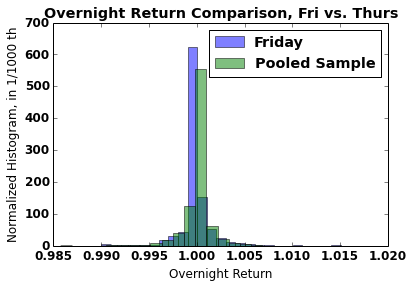
\includegraphics[max size={\textwidth}{\textheight}]{Final_Report_files/Final_Report_86_1.png}
    \par
    \end{center}
    
            \end{InvisibleVerbatim}
            
        
    


    % Make sure that atleast 4 lines are below the HR
    \needspace{4\baselineskip}

    
        \vspace{6pt}
        \makebox[0.1\linewidth]{\smaller\hfill\tt\color{nbframe-in-prompt}In\hspace{4pt}{[}97{]}:\hspace{4pt}}\\*
        \vspace{-2.65\baselineskip}
        \begin{ColorVerbatim}
            \vspace{-0.7\baselineskip}
            \begin{Verbatim}[commandchars=\\\{\}]
\PY{k}{print}\PY{p}{(}\PY{l+s}{\PYZdq{}}\PY{l+s}{Mean of Fridays is}\PY{l+s}{\PYZdq{}}\PY{p}{,} \PY{n}{mean}\PY{p}{(}\PY{n}{Friday}\PY{p}{)}\PY{p}{,} \PY{l+s}{\PYZdq{}}\PY{l+s}{and Mean of Pooled is}\PY{l+s}{\PYZdq{}}\PY{p}{,} \PY{n}{mean}\PY{p}{(}\PY{n}{NonFri}\PY{o}{+}\PY{n}{Friday}\PY{p}{)}\PY{p}{)}
\end{Verbatim}

            
                \vspace{-0.2\baselineskip}
            
        \end{ColorVerbatim}
    

    

        % If the first block is an image, minipage the image.  Else
        % request a certain amount of space for the input text.
        \needspace{4\baselineskip}
        
        

            % Add document contents.
            
                \begin{InvisibleVerbatim}
                \vspace{-0.5\baselineskip}
\begin{alltt}('Mean of Fridays is', 1.0000457911663738, 'and Mean of Pooled is',
0.99996461981281226)
\end{alltt}

            \end{InvisibleVerbatim}
            
        
    


    % Make sure that atleast 4 lines are below the HR
    \needspace{4\baselineskip}

    
        \vspace{6pt}
        \makebox[0.1\linewidth]{\smaller\hfill\tt\color{nbframe-in-prompt}In\hspace{4pt}{[}98{]}:\hspace{4pt}}\\*
        \vspace{-2.65\baselineskip}
        \begin{ColorVerbatim}
            \vspace{-0.7\baselineskip}
            \begin{Verbatim}[commandchars=\\\{\}]
\PY{k}{print}\PY{p}{(}\PY{l+s}{\PYZdq{}}\PY{l+s}{Mean of Pooled is}\PY{l+s}{\PYZdq{}}\PY{p}{,} \PY{n}{mean}\PY{p}{(}\PY{n}{NonFri}\PY{o}{+}\PY{n}{Friday}\PY{p}{)}\PY{p}{)}
\end{Verbatim}

            
                \vspace{-0.2\baselineskip}
            
        \end{ColorVerbatim}
    

    

        % If the first block is an image, minipage the image.  Else
        % request a certain amount of space for the input text.
        \needspace{4\baselineskip}
        
        

            % Add document contents.
            
                \begin{InvisibleVerbatim}
                \vspace{-0.5\baselineskip}
\begin{alltt}('Mean of Pooled is', 0.99996461981281226)
\end{alltt}

            \end{InvisibleVerbatim}
            
        
    
\subsection{Kernel Estimation}\label{kernel-estimation}

Before bootstrapping, we would need to train our kernels such that they
can catch the raw data's distributions closely. In other words, we want
them to be able to reproduce the raw data to the best capacity. Given
the underlying distributions were highly concentrated around 1, we were
not able to choose a Gaussian kernel but had to try a spike-like
``tophat'' kernel.

We start off by simulating the raw data set, and compare-and-constrat if
the reproduced data collide with the original data well. We scratched
new histograms, and observed that the shapes of two histograms almost
perfectly resembled each other, as well as the colors blended.

    % Make sure that atleast 4 lines are below the HR
    \needspace{4\baselineskip}

    
        \vspace{6pt}
        \makebox[0.1\linewidth]{\smaller\hfill\tt\color{nbframe-in-prompt}In\hspace{4pt}{[}99{]}:\hspace{4pt}}\\*
        \vspace{-2.65\baselineskip}
        \begin{ColorVerbatim}
            \vspace{-0.7\baselineskip}
            \begin{Verbatim}[commandchars=\\\{\}]
\PY{k+kn}{from} \PY{n+nn}{sklearn.neighbors} \PY{k+kn}{import} \PY{n}{KernelDensity}
\PY{n}{kde} \PY{o}{=} \PY{n}{KernelDensity}\PY{p}{(}\PY{n}{bandwidth}\PY{o}{=}\PY{o}{.}\PY{l+m+mo}{001}\PY{p}{,} \PY{n}{algorithm}\PY{o}{=}\PY{l+s}{\PYZsq{}}\PY{l+s}{auto}\PY{l+s}{\PYZsq{}}\PY{p}{,} \PY{n}{kernel}\PY{o}{=}\PY{l+s}{\PYZsq{}}\PY{l+s}{tophat}\PY{l+s}{\PYZsq{}}\PY{p}{,} \PY{n}{metric}\PY{o}{=}\PY{l+s}{\PYZsq{}}\PY{l+s}{euclidean}\PY{l+s}{\PYZsq{}}\PY{p}{,} \PY{n}{atol}\PY{o}{=}\PY{l+m+mi}{0}\PY{p}{,} \PY{n}{rtol}\PY{o}{=}\PY{l+m+mi}{0}\PY{p}{,} \PY{n}{breadth\PYZus{}first}\PY{o}{=}\PY{n+nb+bp}{True}\PY{p}{,} \PY{n}{leaf\PYZus{}size}\PY{o}{=}\PY{l+m+mi}{40}\PY{p}{,} \PY{n}{metric\PYZus{}params}\PY{o}{=}\PY{n+nb+bp}{None}\PY{p}{)}
\PY{c}{\PYZsh{} kernel estimation with tophat as spike\PYZhy{}like histogram}

\PY{c}{\PYZsh{} train the model}
\PY{n}{kde}\PY{o}{.}\PY{n}{fit}\PY{p}{(}\PY{n}{Friday}\PY{p}{)}

\PY{c}{\PYZsh{} 100 sample}
\PY{n}{ker100} \PY{o}{=} \PY{n}{kde}\PY{o}{.}\PY{n}{sample}\PY{p}{(}\PY{n}{n\PYZus{}samples}\PY{o}{=}\PY{l+m+mi}{2000}\PY{p}{,} \PY{n}{random\PYZus{}state}\PY{o}{=}\PY{n+nb+bp}{None}\PY{p}{)}

\PY{n}{sample} \PY{o}{=} \PY{p}{[}\PY{p}{]}
\PY{k}{for} \PY{n}{i} \PY{o+ow}{in} \PY{n+nb}{range}\PY{p}{(}\PY{l+m+mi}{0}\PY{p}{,} \PY{n+nb}{len}\PY{p}{(}\PY{n}{ker100}\PY{p}{)}\PY{p}{)}\PY{p}{:}
    \PY{n}{sample} \PY{o}{=} \PY{n}{sample} \PY{o}{+} \PY{n}{ker100}\PY{o}{.}\PY{n}{tolist}\PY{p}{(}\PY{p}{)}\PY{p}{[}\PY{l+m+mi}{0}\PY{p}{]}

\PY{n}{plt}\PY{o}{.}\PY{n}{hist}\PY{p}{(}\PY{n}{Friday}\PY{p}{,} \PY{n}{bins}\PY{o}{=}\PY{l+m+mi}{25}\PY{p}{,} \PY{n}{label}\PY{o}{=}\PY{l+s}{\PYZdq{}}\PY{l+s}{Original Friday}\PY{l+s}{\PYZdq{}}\PY{p}{,} \PY{n}{normed}\PY{o}{=}\PY{n+nb+bp}{True}\PY{p}{,} \PY{n}{alpha}\PY{o}{=}\PY{o}{.}\PY{l+m+mi}{5}\PY{p}{)}
\PY{n}{plt}\PY{o}{.}\PY{n}{hist}\PY{p}{(}\PY{n}{sample}\PY{p}{,} \PY{n}{bins}\PY{o}{=}\PY{l+m+mi}{25}\PY{p}{,} \PY{n}{normed}\PY{o}{=}\PY{n+nb+bp}{True}\PY{p}{,} \PY{n}{label}\PY{o}{=}\PY{l+s}{\PYZdq{}}\PY{l+s}{Kernel Sampled Friday}\PY{l+s}{\PYZdq{}}\PY{p}{,} \PY{n}{alpha}\PY{o}{=}\PY{o}{.}\PY{l+m+mi}{5}\PY{p}{)}  
\PY{c}{\PYZsh{} settled down to Friday\PYZsq{}s}

\PY{n}{plt}\PY{o}{.}\PY{n}{title}\PY{p}{(}\PY{l+s}{\PYZsq{}}\PY{l+s}{Bootstrapping on Friday, N=1000 sampled}\PY{l+s}{\PYZsq{}}\PY{p}{)}
\PY{n}{plt}\PY{o}{.}\PY{n}{ylabel}\PY{p}{(}\PY{l+s}{\PYZsq{}}\PY{l+s}{Normalized Histogram, in 1/1000 th}\PY{l+s}{\PYZsq{}}\PY{p}{)}
\PY{n}{plt}\PY{o}{.}\PY{n}{xlabel}\PY{p}{(}\PY{l+s}{\PYZsq{}}\PY{l+s}{Overnight Return}\PY{l+s}{\PYZsq{}}\PY{p}{)}
\PY{n}{plt}\PY{o}{.}\PY{n}{legend}\PY{p}{(}\PY{n}{loc}\PY{o}{=}\PY{l+m+mi}{0}\PY{p}{)}

\PY{c}{\PYZsh{} kernel estiamted collapse w/ original, so estimation worked}
\end{Verbatim}

            
                \vspace{-0.2\baselineskip}
            
        \end{ColorVerbatim}
    

    

        % If the first block is an image, minipage the image.  Else
        % request a certain amount of space for the input text.
        \needspace{4\baselineskip}
        
        

            % Add document contents.
            
                \makebox[0.1\linewidth]{\smaller\hfill\tt\color{nbframe-out-prompt}Out\hspace{4pt}{[}99{]}:\hspace{4pt}}\\*
                \vspace{-2.55\baselineskip}\begin{InvisibleVerbatim}
                \vspace{-0.5\baselineskip}
\begin{alltt}<matplotlib.legend.Legend at 0x10e08e350>\end{alltt}

            \end{InvisibleVerbatim}
            
                \begin{InvisibleVerbatim}
                \vspace{-0.5\baselineskip}
    \begin{center}
    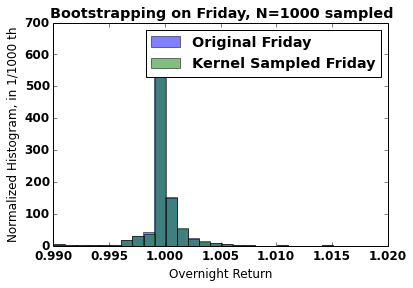
\includegraphics[max size={\textwidth}{\textheight}]{Final_Report_files/Final_Report_90_1.png}
    \par
    \end{center}
    
            \end{InvisibleVerbatim}
            
        
    


    % Make sure that atleast 4 lines are below the HR
    \needspace{4\baselineskip}

    
        \vspace{6pt}
        \makebox[0.1\linewidth]{\smaller\hfill\tt\color{nbframe-in-prompt}In\hspace{4pt}{[}100{]}:\hspace{4pt}}\\*
        \vspace{-2.65\baselineskip}
        \begin{ColorVerbatim}
            \vspace{-0.7\baselineskip}
            \begin{Verbatim}[commandchars=\\\{\}]
\PY{k+kn}{from} \PY{n+nn}{sklearn.neighbors} \PY{k+kn}{import} \PY{n}{KernelDensity}
\PY{n}{kde} \PY{o}{=} \PY{n}{KernelDensity}\PY{p}{(}\PY{n}{bandwidth}\PY{o}{=}\PY{o}{.}\PY{l+m+mo}{001}\PY{p}{,} \PY{n}{algorithm}\PY{o}{=}\PY{l+s}{\PYZsq{}}\PY{l+s}{auto}\PY{l+s}{\PYZsq{}}\PY{p}{,} \PY{n}{kernel}\PY{o}{=}\PY{l+s}{\PYZsq{}}\PY{l+s}{tophat}\PY{l+s}{\PYZsq{}}\PY{p}{,} \PY{n}{metric}\PY{o}{=}\PY{l+s}{\PYZsq{}}\PY{l+s}{euclidean}\PY{l+s}{\PYZsq{}}\PY{p}{,} \PY{n}{atol}\PY{o}{=}\PY{l+m+mi}{0}\PY{p}{,} \PY{n}{rtol}\PY{o}{=}\PY{l+m+mi}{0}\PY{p}{,} \PY{n}{breadth\PYZus{}first}\PY{o}{=}\PY{n+nb+bp}{True}\PY{p}{,} \PY{n}{leaf\PYZus{}size}\PY{o}{=}\PY{l+m+mi}{40}\PY{p}{,} \PY{n}{metric\PYZus{}params}\PY{o}{=}\PY{n+nb+bp}{None}\PY{p}{)}
\PY{c}{\PYZsh{} kernel estimation with tophat as spike\PYZhy{}like histogram}

\PY{c}{\PYZsh{} train the model}
\PY{n}{kde}\PY{o}{.}\PY{n}{fit}\PY{p}{(}\PY{n}{Friday}\PY{o}{+}\PY{n}{NonFri}\PY{p}{)}

\PY{c}{\PYZsh{} 100 sample}
\PY{n}{ker100} \PY{o}{=} \PY{n}{kde}\PY{o}{.}\PY{n}{sample}\PY{p}{(}\PY{n}{n\PYZus{}samples}\PY{o}{=}\PY{l+m+mi}{1000}\PY{p}{,} \PY{n}{random\PYZus{}state}\PY{o}{=}\PY{n+nb+bp}{None}\PY{p}{)}

\PY{n}{sample} \PY{o}{=} \PY{p}{[}\PY{p}{]}
\PY{k}{for} \PY{n}{i} \PY{o+ow}{in} \PY{n+nb}{range}\PY{p}{(}\PY{l+m+mi}{0}\PY{p}{,} \PY{n+nb}{len}\PY{p}{(}\PY{n}{ker100}\PY{p}{)}\PY{p}{)}\PY{p}{:}
    \PY{n}{sample} \PY{o}{=} \PY{n}{sample} \PY{o}{+} \PY{n}{ker100}\PY{o}{.}\PY{n}{tolist}\PY{p}{(}\PY{p}{)}\PY{p}{[}\PY{l+m+mi}{0}\PY{p}{]}

\PY{n}{plt}\PY{o}{.}\PY{n}{hist}\PY{p}{(}\PY{n}{Friday}\PY{o}{+}\PY{n}{NonFri}\PY{p}{,} \PY{n}{bins}\PY{o}{=}\PY{l+m+mi}{25}\PY{p}{,} \PY{n}{label}\PY{o}{=}\PY{l+s}{\PYZdq{}}\PY{l+s}{Original Pooled}\PY{l+s}{\PYZdq{}}\PY{p}{,} \PY{n}{normed}\PY{o}{=}\PY{n+nb+bp}{True}\PY{p}{,} \PY{n}{alpha}\PY{o}{=}\PY{o}{.}\PY{l+m+mi}{5}\PY{p}{)}
\PY{n}{plt}\PY{o}{.}\PY{n}{hist}\PY{p}{(}\PY{n}{sample}\PY{p}{,} \PY{n}{bins}\PY{o}{=}\PY{l+m+mi}{25}\PY{p}{,} \PY{n}{normed}\PY{o}{=}\PY{n+nb+bp}{True}\PY{p}{,} \PY{n}{label}\PY{o}{=}\PY{l+s}{\PYZdq{}}\PY{l+s}{Kernel Sampled}\PY{l+s}{\PYZdq{}}\PY{p}{,} \PY{n}{alpha}\PY{o}{=}\PY{o}{.}\PY{l+m+mi}{5}\PY{p}{)}  \PY{c}{\PYZsh{} settled down to Friday\PYZsq{}s}
\PY{n}{plt}\PY{o}{.}\PY{n}{title}\PY{p}{(}\PY{l+s}{\PYZsq{}}\PY{l+s}{Bootstrapping on Pooled, N=1000 sampled}\PY{l+s}{\PYZsq{}}\PY{p}{)}
\PY{n}{plt}\PY{o}{.}\PY{n}{ylabel}\PY{p}{(}\PY{l+s}{\PYZsq{}}\PY{l+s}{Normalized Histogram, in 1/1000 th}\PY{l+s}{\PYZsq{}}\PY{p}{)}
\PY{n}{plt}\PY{o}{.}\PY{n}{xlabel}\PY{p}{(}\PY{l+s}{\PYZsq{}}\PY{l+s}{Overnight Return}\PY{l+s}{\PYZsq{}}\PY{p}{)}
\PY{n}{plt}\PY{o}{.}\PY{n}{legend}\PY{p}{(}\PY{n}{loc}\PY{o}{=}\PY{l+m+mi}{0}\PY{p}{)}

\PY{c}{\PYZsh{} kernel estiamted collapse w/ original, so estimation worked}
\end{Verbatim}

            
                \vspace{-0.2\baselineskip}
            
        \end{ColorVerbatim}
    

    

        % If the first block is an image, minipage the image.  Else
        % request a certain amount of space for the input text.
        \needspace{4\baselineskip}
        
        

            % Add document contents.
            
                \makebox[0.1\linewidth]{\smaller\hfill\tt\color{nbframe-out-prompt}Out\hspace{4pt}{[}100{]}:\hspace{4pt}}\\*
                \vspace{-2.55\baselineskip}\begin{InvisibleVerbatim}
                \vspace{-0.5\baselineskip}
\begin{alltt}<matplotlib.legend.Legend at 0x10e09f350>\end{alltt}

            \end{InvisibleVerbatim}
            
                \begin{InvisibleVerbatim}
                \vspace{-0.5\baselineskip}
    \begin{center}
    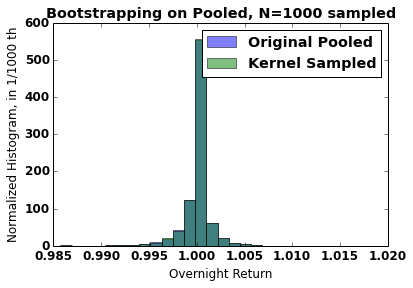
\includegraphics[max size={\textwidth}{\textheight}]{Final_Report_files/Final_Report_91_1.png}
    \par
    \end{center}
    
            \end{InvisibleVerbatim}
            
        
    
\subsection{Bootstrap}\label{bootstrap}

Then, we are able to bootstrap. We defined the bootstrap function to be
the sample mean. Therefore, for each boot, we compute and store the mean
of bootstrapped sample. We first plotted the bootstrapped sample means
of the Friday group and the population group.

The Central Limit Theorem dictates the histogram of boostrapped means to
be normal, which they are.

    % Make sure that atleast 4 lines are below the HR
    \needspace{4\baselineskip}

    
        \vspace{6pt}
        \makebox[0.1\linewidth]{\smaller\hfill\tt\color{nbframe-in-prompt}In\hspace{4pt}{[}101{]}:\hspace{4pt}}\\*
        \vspace{-2.65\baselineskip}
        \begin{ColorVerbatim}
            \vspace{-0.7\baselineskip}
            \begin{Verbatim}[commandchars=\\\{\}]
\PY{n}{MonteCarloBoot} \PY{o}{=} \PY{n}{kde}\PY{o}{.}\PY{n}{sample}\PY{p}{(}\PY{n}{n\PYZus{}samples}\PY{o}{=}\PY{l+m+mi}{1000}\PY{p}{,} \PY{n}{random\PYZus{}state}\PY{o}{=}\PY{n+nb+bp}{None}\PY{p}{)}
\end{Verbatim}

            
                \vspace{-0.2\baselineskip}
            
        \end{ColorVerbatim}
    


    % Make sure that atleast 4 lines are below the HR
    \needspace{4\baselineskip}

    
        \vspace{6pt}
        \makebox[0.1\linewidth]{\smaller\hfill\tt\color{nbframe-in-prompt}In\hspace{4pt}{[}102{]}:\hspace{4pt}}\\*
        \vspace{-2.65\baselineskip}
        \begin{ColorVerbatim}
            \vspace{-0.7\baselineskip}
            \begin{Verbatim}[commandchars=\\\{\}]
\PY{n}{BootMean} \PY{o}{=} \PY{p}{[}\PY{n+nb+bp}{None}\PY{p}{]}\PY{o}{*}\PY{n+nb}{len}\PY{p}{(}\PY{n}{MonteCarloBoot}\PY{p}{)}
\PY{k}{def} \PY{n+nf}{bootMean}\PY{p}{(}\PY{n}{MonteCarloBoot}\PY{p}{,} \PY{n}{BootMean}\PY{p}{)}\PY{p}{:}
    \PY{k}{for} \PY{n}{i} \PY{o+ow}{in} \PY{n+nb}{range}\PY{p}{(}\PY{l+m+mi}{0}\PY{p}{,} \PY{n+nb}{len}\PY{p}{(}\PY{n}{MonteCarloBoot}\PY{p}{)}\PY{p}{)}\PY{p}{:}
        \PY{n}{BootMean}\PY{p}{[}\PY{n}{i}\PY{p}{]} \PY{o}{=} \PY{n}{MonteCarloBoot}\PY{p}{[}\PY{n}{i}\PY{p}{]}\PY{o}{.}\PY{n}{mean}\PY{p}{(}\PY{p}{)}
    \PY{k}{return}\PY{p}{(}\PY{n}{BootMean}\PY{p}{)}

\PY{n}{BootMean} \PY{o}{=} \PY{n}{bootMean}\PY{p}{(}\PY{n}{MonteCarloBoot}\PY{p}{,} \PY{n}{BootMean}\PY{p}{)}

\PY{c}{\PYZsh{} Bootstrapping with T = mean(obs)}
\PY{c}{\PYZsh{} v\PYZus{}boot = 1/B * B\PYZus{}sum(T \PYZhy{} mean(T))\PYZca{}2}

\PY{n}{Boot\PYZus{}var} \PY{o}{=} \PY{n}{std}\PY{p}{(}\PY{n}{BootMean}\PY{p}{)}

\PY{k}{print}\PY{p}{(}\PY{l+s}{\PYZdq{}}\PY{l+s}{Monte Carlo Bootstrapping with mean}\PY{l+s}{\PYZdq{}}\PY{p}{,} \PY{n}{mean}\PY{p}{(}\PY{n}{BootMean}\PY{p}{)}\PY{p}{,} \PY{l+s}{\PYZdq{}}\PY{l+s}{variance}\PY{l+s}{\PYZdq{}}\PY{p}{,} \PY{n}{Boot\PYZus{}var}\PY{p}{)}
\end{Verbatim}

            
                \vspace{-0.2\baselineskip}
            
        \end{ColorVerbatim}
    

    

        % If the first block is an image, minipage the image.  Else
        % request a certain amount of space for the input text.
        \needspace{4\baselineskip}
        
        

            % Add document contents.
            
                \begin{InvisibleVerbatim}
                \vspace{-0.5\baselineskip}
\begin{alltt}('Monte Carlo Bootstrapping with mean', 0.99996463454836415,
'variance', 3.9317659582286139e-07)
\end{alltt}

            \end{InvisibleVerbatim}
            
        
    


    % Make sure that atleast 4 lines are below the HR
    \needspace{4\baselineskip}

    
        \vspace{6pt}
        \makebox[0.1\linewidth]{\smaller\hfill\tt\color{nbframe-in-prompt}In\hspace{4pt}{[}103{]}:\hspace{4pt}}\\*
        \vspace{-2.65\baselineskip}
        \begin{ColorVerbatim}
            \vspace{-0.7\baselineskip}
            \begin{Verbatim}[commandchars=\\\{\}]
\PY{n}{plt}\PY{o}{.}\PY{n}{hist}\PY{p}{(}\PY{n}{BootMean}\PY{p}{,} \PY{n}{bins}\PY{o}{=}\PY{l+m+mi}{25}\PY{p}{,}\PY{n}{normed}\PY{o}{=}\PY{n+nb+bp}{True}\PY{p}{)}
\end{Verbatim}

            
                \vspace{-0.2\baselineskip}
            
        \end{ColorVerbatim}
    

    

        % If the first block is an image, minipage the image.  Else
        % request a certain amount of space for the input text.
        \needspace{4\baselineskip}
        
        

            % Add document contents.
            
                \makebox[0.1\linewidth]{\smaller\hfill\tt\color{nbframe-out-prompt}Out\hspace{4pt}{[}103{]}:\hspace{4pt}}\\*
                \vspace{-2.55\baselineskip}\begin{InvisibleVerbatim}
                \vspace{-0.5\baselineskip}
\begin{alltt}(array([    9319.26375747,    18638.52751494,    27957.79127242,
          55915.58254483,    65234.8463698 ,   130469.69260461,
         214343.06642187,   419366.86908626,   559155.82544835,
         726902.57308285,   941245.63950472,  1081034.5958668 ,
        1108992.38828663,   792137.41938516,   792137.41938516,
         605752.14423571,   633709.93550813,   521878.77041846,
         279577.91272417,   149108.22011956,    83873.37390403,
          46596.31878736,    46596.31878736,        0.        ,
           9319.26375747]),
 array([ 0.99996329,  0.9999634 ,  0.9999635 ,  0.99996361,
0.99996372,
        0.99996382,  0.99996393,  0.99996404,  0.99996415,
0.99996425,
        0.99996436,  0.99996447,  0.99996458,  0.99996468,
0.99996479,
        0.9999649 ,  0.999965  ,  0.99996511,  0.99996522,
0.99996533,
        0.99996543,  0.99996554,  0.99996565,  0.99996576,
0.99996586,
        0.99996597]),
 <a list of 25 Patch objects>)\end{alltt}

            \end{InvisibleVerbatim}
            
                \begin{InvisibleVerbatim}
                \vspace{-0.5\baselineskip}
    \begin{center}
    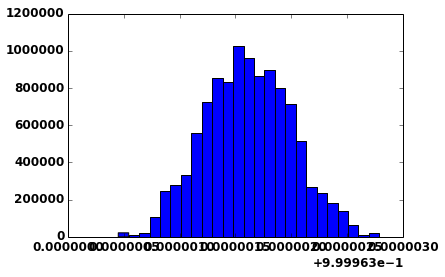
\includegraphics[max size={\textwidth}{\textheight}]{Final_Report_files/Final_Report_95_1.png}
    \par
    \end{center}
    
            \end{InvisibleVerbatim}
            
        
    


    % Make sure that atleast 4 lines are below the HR
    \needspace{4\baselineskip}

    
        \vspace{6pt}
        \makebox[0.1\linewidth]{\smaller\hfill\tt\color{nbframe-in-prompt}In\hspace{4pt}{[}104{]}:\hspace{4pt}}\\*
        \vspace{-2.65\baselineskip}
        \begin{ColorVerbatim}
            \vspace{-0.7\baselineskip}
            \begin{Verbatim}[commandchars=\\\{\}]
\PY{k+kn}{from} \PY{n+nn}{sklearn.neighbors} \PY{k+kn}{import} \PY{n}{KernelDensity}
\PY{c}{\PYZsh{} kernel estimation with tophat as spike\PYZhy{}like histogram}

\PY{c}{\PYZsh{}\PYZsh{}\PYZsh{}\PYZsh{}\PYZsh{}\PYZsh{}\PYZsh{}\PYZsh{}\PYZsh{}\PYZsh{}\PYZsh{}\PYZsh{}\PYZsh{}\PYZsh{}\PYZsh{}\PYZsh{}\PYZsh{}\PYZsh{}\PYZsh{}\PYZsh{}\PYZsh{}\PYZsh{}\PYZsh{}\PYZsh{}\PYZsh{}\PYZsh{}\PYZsh{}\PYZsh{} Friday \PYZsh{}\PYZsh{}\PYZsh{}\PYZsh{}\PYZsh{}\PYZsh{}\PYZsh{}\PYZsh{}\PYZsh{}\PYZsh{}\PYZsh{}\PYZsh{}\PYZsh{}\PYZsh{}\PYZsh{}\PYZsh{}\PYZsh{}\PYZsh{}\PYZsh{}\PYZsh{}\PYZsh{}\PYZsh{}\PYZsh{}\PYZsh{}\PYZsh{}\PYZsh{}\PYZsh{}\PYZsh{}}

\PY{n}{kdeF} \PY{o}{=} \PY{n}{KernelDensity}\PY{p}{(}\PY{n}{bandwidth}\PY{o}{=}\PY{o}{.}\PY{l+m+mo}{001}\PY{p}{,} \PY{n}{algorithm}\PY{o}{=}\PY{l+s}{\PYZsq{}}\PY{l+s}{auto}\PY{l+s}{\PYZsq{}}\PY{p}{,} \PY{n}{kernel}\PY{o}{=}\PY{l+s}{\PYZsq{}}\PY{l+s}{tophat}\PY{l+s}{\PYZsq{}}\PY{p}{,} \PY{n}{metric}\PY{o}{=}\PY{l+s}{\PYZsq{}}\PY{l+s}{euclidean}\PY{l+s}{\PYZsq{}}\PY{p}{,} \PY{n}{atol}\PY{o}{=}\PY{l+m+mi}{0}\PY{p}{,} \PY{n}{rtol}\PY{o}{=}\PY{l+m+mi}{0}\PY{p}{,} \PY{n}{breadth\PYZus{}first}\PY{o}{=}\PY{n+nb+bp}{True}\PY{p}{,} \PY{n}{leaf\PYZus{}size}\PY{o}{=}\PY{l+m+mi}{40}\PY{p}{,} \PY{n}{metric\PYZus{}params}\PY{o}{=}\PY{n+nb+bp}{None}\PY{p}{)}

\PY{n}{kdeF}\PY{o}{.}\PY{n}{fit}\PY{p}{(}\PY{n}{Friday}\PY{p}{)}
\PY{n}{FriBoot} \PY{o}{=} \PY{n}{kdeF}\PY{o}{.}\PY{n}{sample}\PY{p}{(}\PY{n}{n\PYZus{}samples}\PY{o}{=}\PY{l+m+mi}{1000}\PY{p}{,} \PY{n}{random\PYZus{}state}\PY{o}{=}\PY{n+nb+bp}{None}\PY{p}{)}

\PY{n}{FriBootMean} \PY{o}{=} \PY{p}{[}\PY{n+nb+bp}{None}\PY{p}{]}\PY{o}{*}\PY{n+nb}{len}\PY{p}{(}\PY{n}{FriBoot}\PY{p}{)}
\PY{n}{FriBootMean} \PY{o}{=} \PY{n}{bootMean}\PY{p}{(}\PY{n}{FriBoot}\PY{p}{,} \PY{n}{FriBootMean}\PY{p}{)}

\PY{c}{\PYZsh{}\PYZsh{}\PYZsh{}\PYZsh{}\PYZsh{}\PYZsh{}\PYZsh{}\PYZsh{}\PYZsh{}\PYZsh{}\PYZsh{}\PYZsh{}\PYZsh{}\PYZsh{}\PYZsh{}\PYZsh{}\PYZsh{}\PYZsh{}\PYZsh{}\PYZsh{}\PYZsh{}\PYZsh{}\PYZsh{}\PYZsh{}\PYZsh{}\PYZsh{}\PYZsh{}\PYZsh{} Thursday \PYZsh{}\PYZsh{}\PYZsh{}\PYZsh{}\PYZsh{}\PYZsh{}\PYZsh{}\PYZsh{}\PYZsh{}\PYZsh{}\PYZsh{}\PYZsh{}\PYZsh{}\PYZsh{}\PYZsh{}\PYZsh{}\PYZsh{}\PYZsh{}\PYZsh{}\PYZsh{}\PYZsh{}\PYZsh{}\PYZsh{}\PYZsh{}\PYZsh{}\PYZsh{}\PYZsh{}\PYZsh{}}

\PY{n}{kdeR} \PY{o}{=} \PY{n}{KernelDensity}\PY{p}{(}\PY{n}{bandwidth}\PY{o}{=}\PY{o}{.}\PY{l+m+mo}{001}\PY{p}{,} \PY{n}{algorithm}\PY{o}{=}\PY{l+s}{\PYZsq{}}\PY{l+s}{auto}\PY{l+s}{\PYZsq{}}\PY{p}{,} \PY{n}{kernel}\PY{o}{=}\PY{l+s}{\PYZsq{}}\PY{l+s}{tophat}\PY{l+s}{\PYZsq{}}\PY{p}{,} \PY{n}{metric}\PY{o}{=}\PY{l+s}{\PYZsq{}}\PY{l+s}{euclidean}\PY{l+s}{\PYZsq{}}\PY{p}{,} \PY{n}{atol}\PY{o}{=}\PY{l+m+mi}{0}\PY{p}{,} \PY{n}{rtol}\PY{o}{=}\PY{l+m+mi}{0}\PY{p}{,} \PY{n}{breadth\PYZus{}first}\PY{o}{=}\PY{n+nb+bp}{True}\PY{p}{,} \PY{n}{leaf\PYZus{}size}\PY{o}{=}\PY{l+m+mi}{40}\PY{p}{,} \PY{n}{metric\PYZus{}params}\PY{o}{=}\PY{n+nb+bp}{None}\PY{p}{)}

\PY{n}{kdeR}\PY{o}{.}\PY{n}{fit}\PY{p}{(}\PY{n}{Thursday}\PY{p}{)}
\PY{n}{ThrBoot} \PY{o}{=} \PY{n}{kdeR}\PY{o}{.}\PY{n}{sample}\PY{p}{(}\PY{n}{n\PYZus{}samples}\PY{o}{=}\PY{l+m+mi}{1000}\PY{p}{,} \PY{n}{random\PYZus{}state}\PY{o}{=}\PY{n+nb+bp}{None}\PY{p}{)}

\PY{n}{ThrBootMean} \PY{o}{=} \PY{p}{[}\PY{n+nb+bp}{None}\PY{p}{]}\PY{o}{*}\PY{n+nb}{len}\PY{p}{(}\PY{n}{ThrBoot}\PY{p}{)}
\PY{n}{ThrBootMean} \PY{o}{=} \PY{n}{bootMean}\PY{p}{(}\PY{n}{ThrBoot}\PY{p}{,} \PY{n}{ThrBootMean}\PY{p}{)}


\PY{c}{\PYZsh{}\PYZsh{}\PYZsh{}\PYZsh{}\PYZsh{}\PYZsh{}\PYZsh{}\PYZsh{}\PYZsh{}\PYZsh{}\PYZsh{}\PYZsh{}\PYZsh{}\PYZsh{}\PYZsh{}\PYZsh{}\PYZsh{}\PYZsh{}\PYZsh{}\PYZsh{}\PYZsh{}\PYZsh{}\PYZsh{}\PYZsh{}\PYZsh{}\PYZsh{}\PYZsh{}\PYZsh{} Wednesday \PYZsh{}\PYZsh{}\PYZsh{}\PYZsh{}\PYZsh{}\PYZsh{}\PYZsh{}\PYZsh{}\PYZsh{}\PYZsh{}\PYZsh{}\PYZsh{}\PYZsh{}\PYZsh{}\PYZsh{}\PYZsh{}\PYZsh{}\PYZsh{}\PYZsh{}\PYZsh{}\PYZsh{}\PYZsh{}\PYZsh{}\PYZsh{}\PYZsh{}\PYZsh{}\PYZsh{}\PYZsh{}}


\PY{n}{kdeW} \PY{o}{=} \PY{n}{KernelDensity}\PY{p}{(}\PY{n}{bandwidth}\PY{o}{=}\PY{o}{.}\PY{l+m+mo}{001}\PY{p}{,} \PY{n}{algorithm}\PY{o}{=}\PY{l+s}{\PYZsq{}}\PY{l+s}{auto}\PY{l+s}{\PYZsq{}}\PY{p}{,} \PY{n}{kernel}\PY{o}{=}\PY{l+s}{\PYZsq{}}\PY{l+s}{tophat}\PY{l+s}{\PYZsq{}}\PY{p}{,} \PY{n}{metric}\PY{o}{=}\PY{l+s}{\PYZsq{}}\PY{l+s}{euclidean}\PY{l+s}{\PYZsq{}}\PY{p}{,} \PY{n}{atol}\PY{o}{=}\PY{l+m+mi}{0}\PY{p}{,} \PY{n}{rtol}\PY{o}{=}\PY{l+m+mi}{0}\PY{p}{,} \PY{n}{breadth\PYZus{}first}\PY{o}{=}\PY{n+nb+bp}{True}\PY{p}{,} \PY{n}{leaf\PYZus{}size}\PY{o}{=}\PY{l+m+mi}{40}\PY{p}{,} \PY{n}{metric\PYZus{}params}\PY{o}{=}\PY{n+nb+bp}{None}\PY{p}{)}

\PY{n}{kdeW}\PY{o}{.}\PY{n}{fit}\PY{p}{(}\PY{n}{Wednesday}\PY{p}{)}
\PY{n}{WedBoot} \PY{o}{=} \PY{n}{kdeW}\PY{o}{.}\PY{n}{sample}\PY{p}{(}\PY{n}{n\PYZus{}samples}\PY{o}{=}\PY{l+m+mi}{1000}\PY{p}{,} \PY{n}{random\PYZus{}state}\PY{o}{=}\PY{n+nb+bp}{None}\PY{p}{)}

\PY{n}{WedBootMean} \PY{o}{=} \PY{p}{[}\PY{n+nb+bp}{None}\PY{p}{]}\PY{o}{*}\PY{n+nb}{len}\PY{p}{(}\PY{n}{WedBoot}\PY{p}{)}
\PY{n}{WedBootMean} \PY{o}{=} \PY{n}{bootMean}\PY{p}{(}\PY{n}{WedBoot}\PY{p}{,} \PY{n}{WedBootMean}\PY{p}{)}

\PY{c}{\PYZsh{}\PYZsh{}\PYZsh{}\PYZsh{}\PYZsh{}\PYZsh{}\PYZsh{}\PYZsh{}\PYZsh{}\PYZsh{}\PYZsh{}\PYZsh{}\PYZsh{}\PYZsh{}\PYZsh{}\PYZsh{}\PYZsh{}\PYZsh{}\PYZsh{}\PYZsh{}\PYZsh{}\PYZsh{}\PYZsh{}\PYZsh{}\PYZsh{}\PYZsh{}\PYZsh{}\PYZsh{} Tuesday \PYZsh{}\PYZsh{}\PYZsh{}\PYZsh{}\PYZsh{}\PYZsh{}\PYZsh{}\PYZsh{}\PYZsh{}\PYZsh{}\PYZsh{}\PYZsh{}\PYZsh{}\PYZsh{}\PYZsh{}\PYZsh{}\PYZsh{}\PYZsh{}\PYZsh{}\PYZsh{}\PYZsh{}\PYZsh{}\PYZsh{}\PYZsh{}\PYZsh{}\PYZsh{}\PYZsh{}\PYZsh{}}


\PY{n}{kdeT} \PY{o}{=} \PY{n}{KernelDensity}\PY{p}{(}\PY{n}{bandwidth}\PY{o}{=}\PY{o}{.}\PY{l+m+mo}{001}\PY{p}{,} \PY{n}{algorithm}\PY{o}{=}\PY{l+s}{\PYZsq{}}\PY{l+s}{auto}\PY{l+s}{\PYZsq{}}\PY{p}{,} \PY{n}{kernel}\PY{o}{=}\PY{l+s}{\PYZsq{}}\PY{l+s}{tophat}\PY{l+s}{\PYZsq{}}\PY{p}{,} \PY{n}{metric}\PY{o}{=}\PY{l+s}{\PYZsq{}}\PY{l+s}{euclidean}\PY{l+s}{\PYZsq{}}\PY{p}{,} \PY{n}{atol}\PY{o}{=}\PY{l+m+mi}{0}\PY{p}{,} \PY{n}{rtol}\PY{o}{=}\PY{l+m+mi}{0}\PY{p}{,} \PY{n}{breadth\PYZus{}first}\PY{o}{=}\PY{n+nb+bp}{True}\PY{p}{,} \PY{n}{leaf\PYZus{}size}\PY{o}{=}\PY{l+m+mi}{40}\PY{p}{,} \PY{n}{metric\PYZus{}params}\PY{o}{=}\PY{n+nb+bp}{None}\PY{p}{)}

\PY{n}{kdeT}\PY{o}{.}\PY{n}{fit}\PY{p}{(}\PY{n}{Wednesday}\PY{p}{)}
\PY{n}{TueBoot} \PY{o}{=} \PY{n}{kdeT}\PY{o}{.}\PY{n}{sample}\PY{p}{(}\PY{n}{n\PYZus{}samples}\PY{o}{=}\PY{l+m+mi}{1000}\PY{p}{,} \PY{n}{random\PYZus{}state}\PY{o}{=}\PY{n+nb+bp}{None}\PY{p}{)}

\PY{n}{TueBootMean} \PY{o}{=} \PY{p}{[}\PY{n+nb+bp}{None}\PY{p}{]}\PY{o}{*}\PY{n+nb}{len}\PY{p}{(}\PY{n}{TueBoot}\PY{p}{)}
\PY{n}{TueBootMean} \PY{o}{=} \PY{n}{bootMean}\PY{p}{(}\PY{n}{TueBoot}\PY{p}{,} \PY{n}{TueBootMean}\PY{p}{)}

\PY{c}{\PYZsh{}\PYZsh{}\PYZsh{}\PYZsh{}\PYZsh{}\PYZsh{}\PYZsh{}\PYZsh{}\PYZsh{}\PYZsh{}\PYZsh{}\PYZsh{}\PYZsh{}\PYZsh{}\PYZsh{}\PYZsh{}\PYZsh{}\PYZsh{}\PYZsh{}\PYZsh{}\PYZsh{}\PYZsh{}\PYZsh{}\PYZsh{}\PYZsh{}\PYZsh{}\PYZsh{}\PYZsh{} Monday \PYZsh{}\PYZsh{}\PYZsh{}\PYZsh{}\PYZsh{}\PYZsh{}\PYZsh{}\PYZsh{}\PYZsh{}\PYZsh{}\PYZsh{}\PYZsh{}\PYZsh{}\PYZsh{}\PYZsh{}\PYZsh{}\PYZsh{}\PYZsh{}\PYZsh{}\PYZsh{}\PYZsh{}\PYZsh{}\PYZsh{}\PYZsh{}\PYZsh{}\PYZsh{}\PYZsh{}\PYZsh{}}


\PY{n}{kdeM} \PY{o}{=} \PY{n}{KernelDensity}\PY{p}{(}\PY{n}{bandwidth}\PY{o}{=}\PY{o}{.}\PY{l+m+mo}{001}\PY{p}{,} \PY{n}{algorithm}\PY{o}{=}\PY{l+s}{\PYZsq{}}\PY{l+s}{auto}\PY{l+s}{\PYZsq{}}\PY{p}{,} \PY{n}{kernel}\PY{o}{=}\PY{l+s}{\PYZsq{}}\PY{l+s}{tophat}\PY{l+s}{\PYZsq{}}\PY{p}{,} \PY{n}{metric}\PY{o}{=}\PY{l+s}{\PYZsq{}}\PY{l+s}{euclidean}\PY{l+s}{\PYZsq{}}\PY{p}{,} \PY{n}{atol}\PY{o}{=}\PY{l+m+mi}{0}\PY{p}{,} \PY{n}{rtol}\PY{o}{=}\PY{l+m+mi}{0}\PY{p}{,} \PY{n}{breadth\PYZus{}first}\PY{o}{=}\PY{n+nb+bp}{True}\PY{p}{,} \PY{n}{leaf\PYZus{}size}\PY{o}{=}\PY{l+m+mi}{40}\PY{p}{,} \PY{n}{metric\PYZus{}params}\PY{o}{=}\PY{n+nb+bp}{None}\PY{p}{)}

\PY{n}{kdeM}\PY{o}{.}\PY{n}{fit}\PY{p}{(}\PY{n}{Monday}\PY{p}{)}
\PY{n}{MonBoot} \PY{o}{=} \PY{n}{kdeM}\PY{o}{.}\PY{n}{sample}\PY{p}{(}\PY{n}{n\PYZus{}samples}\PY{o}{=}\PY{l+m+mi}{1000}\PY{p}{,} \PY{n}{random\PYZus{}state}\PY{o}{=}\PY{n+nb+bp}{None}\PY{p}{)}

\PY{n}{MonBootMean} \PY{o}{=} \PY{p}{[}\PY{n+nb+bp}{None}\PY{p}{]}\PY{o}{*}\PY{n+nb}{len}\PY{p}{(}\PY{n}{MonBoot}\PY{p}{)}
\PY{n}{MonBootMean} \PY{o}{=} \PY{n}{bootMean}\PY{p}{(}\PY{n}{MonBoot}\PY{p}{,} \PY{n}{MonBootMean}\PY{p}{)}

    
\PY{c}{\PYZsh{} plt.hist(FriBootMean, bins=25,normed=True)}
\end{Verbatim}

            
                \vspace{-0.2\baselineskip}
            
        \end{ColorVerbatim}
    


    % Make sure that atleast 4 lines are below the HR
    \needspace{4\baselineskip}

    
        \vspace{6pt}
        \makebox[0.1\linewidth]{\smaller\hfill\tt\color{nbframe-in-prompt}In\hspace{4pt}{[}105{]}:\hspace{4pt}}\\*
        \vspace{-2.65\baselineskip}
        \begin{ColorVerbatim}
            \vspace{-0.7\baselineskip}
            \begin{Verbatim}[commandchars=\\\{\}]
\PY{n}{plt}\PY{o}{.}\PY{n}{hist}\PY{p}{(}\PY{n}{FriBootMean}\PY{p}{,} \PY{l+m+mi}{25}\PY{p}{,} \PY{n}{label}\PY{o}{=}\PY{l+s}{\PYZdq{}}\PY{l+s}{Fri}\PY{l+s}{\PYZdq{}}\PY{p}{,} \PY{n}{alpha}\PY{o}{=}\PY{o}{.}\PY{l+m+mi}{5}\PY{p}{,} \PY{n}{normed}\PY{o}{=}\PY{n+nb+bp}{True}\PY{p}{)}
\PY{c}{\PYZsh{}plt.hist(ThrBootMean, 25, label=\PYZdq{}Thr\PYZdq{}, alpha=.5, normed=True)}
\PY{c}{\PYZsh{}plt.hist(WedBootMean, 25, label=\PYZdq{}Wed\PYZdq{}, alpha=.5, normed=True)}
\PY{c}{\PYZsh{}plt.hist(TueBootMean, 25, label=\PYZdq{}Tue\PYZdq{}, alpha=.5, normed=True)}
\PY{c}{\PYZsh{}plt.hist(MonBootMean, 25, label=\PYZdq{}Mon\PYZdq{}, alpha=.5,normed=True)}
\PY{c}{\PYZsh{}plt.hist(BootMean, 25, label=\PYZdq{}Pooled\PYZdq{}, alpha=.5, normed=True)}
\PY{n}{plt}\PY{o}{.}\PY{n}{legend}\PY{p}{(}\PY{n}{loc}\PY{o}{=}\PY{l+m+mi}{0}\PY{p}{)}
\PY{n}{plt}\PY{o}{.}\PY{n}{ticklabel\PYZus{}format}\PY{p}{(}\PY{n}{style}\PY{o}{=}\PY{l+s}{\PYZsq{}}\PY{l+s}{plain}\PY{l+s}{\PYZsq{}}\PY{p}{,} \PY{n}{axis}\PY{o}{=}\PY{l+s}{\PYZsq{}}\PY{l+s}{x}\PY{l+s}{\PYZsq{}}\PY{p}{,} \PY{n}{scilimits}\PY{o}{=}\PY{p}{(}\PY{l+m+mi}{0}\PY{p}{,}\PY{l+m+mi}{0}\PY{p}{)}\PY{p}{)}
\PY{n}{plt}\PY{o}{.}\PY{n}{title}\PY{p}{(}\PY{l+s}{\PYZsq{}}\PY{l+s}{Bootstrap on g(T) = Sample Mean}\PY{l+s}{\PYZsq{}}\PY{p}{)}
\PY{n}{plt}\PY{o}{.}\PY{n}{ylabel}\PY{p}{(}\PY{l+s}{\PYZsq{}}\PY{l+s}{Normalized Histogram, in 1/10000000 th}\PY{l+s}{\PYZsq{}}\PY{p}{)}
\PY{n}{plt}\PY{o}{.}\PY{n}{xlabel}\PY{p}{(}\PY{l+s}{\PYZsq{}}\PY{l+s}{Overnight Return}\PY{l+s}{\PYZsq{}}\PY{p}{)}
\PY{c}{\PYZsh{}plt.ylim((0,300000))}
\PY{n}{show}\PY{p}{(}\PY{p}{)}
\end{Verbatim}

            
                \vspace{-0.2\baselineskip}
            
        \end{ColorVerbatim}
    

    

        % If the first block is an image, minipage the image.  Else
        % request a certain amount of space for the input text.
        \needspace{4\baselineskip}
        
        

            % Add document contents.
            
                \begin{InvisibleVerbatim}
                \vspace{-0.5\baselineskip}
    \begin{center}
    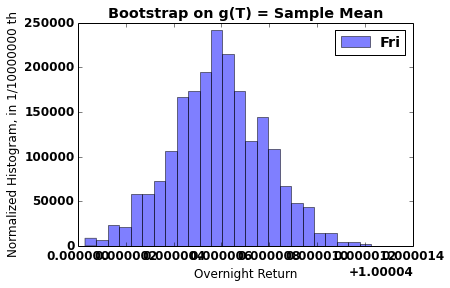
\includegraphics[max size={\textwidth}{\textheight}]{Final_Report_files/Final_Report_97_0.png}
    \par
    \end{center}
    
            \end{InvisibleVerbatim}
            
        
    
\subsection{Bootstrap Results}\label{bootstrap-results}

Monte Carlo Simulation indicates that Friday has different distribution
pattern from other days of the week combined. Surprisingly, the Friday
group came up the most positive.

To better understand the following plots, notice that

\begin{enumerate}
\def\labelenumi{\arabic{enumi})}
\itemsep1pt\parskip0pt\parsep0pt
\item
  There are six histograms being plotted on the same picture, but two of
  which overlapped.
\item
  The tallest and skinest one is the boot mean of the population. As it
  had five times as many size of the others, its standard error shrinks
  to by one over square root of five. Hence, it had a much smaller
  variability that results a different shape.
\item
  Among five ``day of the week'' individual boots, Friday had the
  highest boot means. In other words, Fridays over the last ten years
  were probably doing better than the rest weekdays.
\item
  To better see the comparison, notice a cleaner plot underneath the
  summary plot.
\end{enumerate}

    % Make sure that atleast 4 lines are below the HR
    \needspace{4\baselineskip}

    
        \vspace{6pt}
        \makebox[0.1\linewidth]{\smaller\hfill\tt\color{nbframe-in-prompt}In\hspace{4pt}{[}106{]}:\hspace{4pt}}\\*
        \vspace{-2.65\baselineskip}
        \begin{ColorVerbatim}
            \vspace{-0.7\baselineskip}
            \begin{Verbatim}[commandchars=\\\{\}]
\PY{n}{plt}\PY{o}{.}\PY{n}{hist}\PY{p}{(}\PY{n}{FriBootMean}\PY{p}{,} \PY{l+m+mi}{25}\PY{p}{,} \PY{n}{label}\PY{o}{=}\PY{l+s}{\PYZdq{}}\PY{l+s}{Fri}\PY{l+s}{\PYZdq{}}\PY{p}{,} \PY{n}{alpha}\PY{o}{=}\PY{o}{.}\PY{l+m+mi}{5}\PY{p}{,} \PY{n}{normed}\PY{o}{=}\PY{n+nb+bp}{True}\PY{p}{)}
\PY{n}{plt}\PY{o}{.}\PY{n}{hist}\PY{p}{(}\PY{n}{ThrBootMean}\PY{p}{,} \PY{l+m+mi}{25}\PY{p}{,} \PY{n}{label}\PY{o}{=}\PY{l+s}{\PYZdq{}}\PY{l+s}{Thr}\PY{l+s}{\PYZdq{}}\PY{p}{,}  \PY{n}{alpha}\PY{o}{=}\PY{o}{.}\PY{l+m+mi}{5}\PY{p}{,} \PY{n}{normed}\PY{o}{=}\PY{n+nb+bp}{True}\PY{p}{)}
\PY{n}{plt}\PY{o}{.}\PY{n}{hist}\PY{p}{(}\PY{n}{WedBootMean}\PY{p}{,} \PY{l+m+mi}{25}\PY{p}{,} \PY{n}{label}\PY{o}{=}\PY{l+s}{\PYZdq{}}\PY{l+s}{Wed}\PY{l+s}{\PYZdq{}}\PY{p}{,}  \PY{n}{alpha}\PY{o}{=}\PY{o}{.}\PY{l+m+mi}{5}\PY{p}{,} \PY{n}{normed}\PY{o}{=}\PY{n+nb+bp}{True}\PY{p}{)}
\PY{n}{plt}\PY{o}{.}\PY{n}{hist}\PY{p}{(}\PY{n}{TueBootMean}\PY{p}{,} \PY{l+m+mi}{25}\PY{p}{,} \PY{n}{label}\PY{o}{=}\PY{l+s}{\PYZdq{}}\PY{l+s}{Tue}\PY{l+s}{\PYZdq{}}\PY{p}{,}  \PY{n}{alpha}\PY{o}{=}\PY{o}{.}\PY{l+m+mi}{5}\PY{p}{,} \PY{n}{normed}\PY{o}{=}\PY{n+nb+bp}{True}\PY{p}{)}
\PY{n}{plt}\PY{o}{.}\PY{n}{hist}\PY{p}{(}\PY{n}{MonBootMean}\PY{p}{,} \PY{l+m+mi}{25}\PY{p}{,} \PY{n}{label}\PY{o}{=}\PY{l+s}{\PYZdq{}}\PY{l+s}{Mon}\PY{l+s}{\PYZdq{}}\PY{p}{,}  \PY{n}{alpha}\PY{o}{=}\PY{l+m+mf}{0.5}\PY{p}{,}\PY{n}{normed}\PY{o}{=}\PY{n+nb+bp}{True}\PY{p}{)}
\PY{n}{plt}\PY{o}{.}\PY{n}{hist}\PY{p}{(}\PY{n}{BootMean}\PY{p}{,} \PY{l+m+mi}{25}\PY{p}{,} \PY{n}{label}\PY{o}{=}\PY{l+s}{\PYZdq{}}\PY{l+s}{Pooled}\PY{l+s}{\PYZdq{}}\PY{p}{,}  \PY{n}{alpha}\PY{o}{=}\PY{o}{.}\PY{l+m+mi}{5}\PY{p}{,} \PY{n}{normed}\PY{o}{=}\PY{n+nb+bp}{True}\PY{p}{)}
\PY{n}{plt}\PY{o}{.}\PY{n}{title}\PY{p}{(}\PY{l+s}{\PYZsq{}}\PY{l+s}{Zoomed in Bootstrap}\PY{l+s}{\PYZsq{}}\PY{p}{)}
\PY{n}{plt}\PY{o}{.}\PY{n}{ylabel}\PY{p}{(}\PY{l+s}{\PYZsq{}}\PY{l+s}{Normalized Histogram, in 1/1000000 th}\PY{l+s}{\PYZsq{}}\PY{p}{)}
\PY{n}{plt}\PY{o}{.}\PY{n}{xlabel}\PY{p}{(}\PY{l+s}{\PYZsq{}}\PY{l+s}{Overnight Return}\PY{l+s}{\PYZsq{}}\PY{p}{)}
\PY{n}{plt}\PY{o}{.}\PY{n}{legend}\PY{p}{(}\PY{n}{loc}\PY{o}{=}\PY{l+m+mi}{0}\PY{p}{)}
\PY{c}{\PYZsh{}plt.ylim((0,300000))}
\PY{n}{show}\PY{p}{(}\PY{p}{)}
\end{Verbatim}

            
                \vspace{-0.2\baselineskip}
            
        \end{ColorVerbatim}
    

    

        % If the first block is an image, minipage the image.  Else
        % request a certain amount of space for the input text.
        \needspace{4\baselineskip}
        
        

            % Add document contents.
            
                \begin{InvisibleVerbatim}
                \vspace{-0.5\baselineskip}
    \begin{center}
    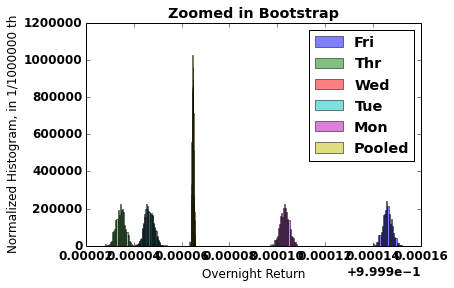
\includegraphics[max size={\textwidth}{\textheight}]{Final_Report_files/Final_Report_99_0.png}
    \par
    \end{center}
    
            \end{InvisibleVerbatim}
            
        
    


    % Make sure that atleast 4 lines are below the HR
    \needspace{4\baselineskip}

    
        \vspace{6pt}
        \makebox[0.1\linewidth]{\smaller\hfill\tt\color{nbframe-in-prompt}In\hspace{4pt}{[}107{]}:\hspace{4pt}}\\*
        \vspace{-2.65\baselineskip}
        \begin{ColorVerbatim}
            \vspace{-0.7\baselineskip}
            \begin{Verbatim}[commandchars=\\\{\}]
\PY{n}{plt}\PY{o}{.}\PY{n}{hist}\PY{p}{(}\PY{n}{FriBootMean}\PY{p}{,} \PY{l+m+mi}{25}\PY{p}{,} \PY{n}{label}\PY{o}{=}\PY{l+s}{\PYZdq{}}\PY{l+s}{Fri}\PY{l+s}{\PYZdq{}}\PY{p}{,} \PY{n}{alpha}\PY{o}{=}\PY{o}{.}\PY{l+m+mi}{5}\PY{p}{,} \PY{n}{normed}\PY{o}{=}\PY{n+nb+bp}{True}\PY{p}{)}
\PY{n}{plt}\PY{o}{.}\PY{n}{hist}\PY{p}{(}\PY{n}{ThrBootMean}\PY{p}{,} \PY{l+m+mi}{25}\PY{p}{,} \PY{n}{label}\PY{o}{=}\PY{l+s}{\PYZdq{}}\PY{l+s}{Thr}\PY{l+s}{\PYZdq{}}\PY{p}{,} \PY{n}{alpha}\PY{o}{=}\PY{o}{.}\PY{l+m+mi}{5}\PY{p}{,} \PY{n}{normed}\PY{o}{=}\PY{n+nb+bp}{True}\PY{p}{)}
\PY{c}{\PYZsh{}plt.hist(WedBootMean, 25, label=\PYZdq{}Wed\PYZdq{}, alpha=.5, normed=True)}
\PY{c}{\PYZsh{}plt.hist(TueBootMean, 25, label=\PYZdq{}Tue\PYZdq{}, alpha=.5, normed=True)}
\PY{c}{\PYZsh{}plt.hist(MonBootMean, 25, label=\PYZdq{}Mon\PYZdq{}, alpha=0.5,normed=True)}
\PY{n}{plt}\PY{o}{.}\PY{n}{hist}\PY{p}{(}\PY{n}{BootMean}\PY{p}{,} \PY{l+m+mi}{25}\PY{p}{,} \PY{n}{label}\PY{o}{=}\PY{l+s}{\PYZdq{}}\PY{l+s}{Pooled}\PY{l+s}{\PYZdq{}}\PY{p}{,} \PY{n}{alpha}\PY{o}{=}\PY{o}{.}\PY{l+m+mi}{5}\PY{p}{,} \PY{n}{normed}\PY{o}{=}\PY{n+nb+bp}{True}\PY{p}{)}
\PY{n}{plt}\PY{o}{.}\PY{n}{title}\PY{p}{(}\PY{l+s}{\PYZsq{}}\PY{l+s}{Reduced Bootstrap}\PY{l+s}{\PYZsq{}}\PY{p}{)}
\PY{n}{plt}\PY{o}{.}\PY{n}{ylabel}\PY{p}{(}\PY{l+s}{\PYZsq{}}\PY{l+s}{Normalized Histogram, in 1/1000000 th}\PY{l+s}{\PYZsq{}}\PY{p}{)}
\PY{n}{plt}\PY{o}{.}\PY{n}{xlabel}\PY{p}{(}\PY{l+s}{\PYZsq{}}\PY{l+s}{Overnight Return}\PY{l+s}{\PYZsq{}}\PY{p}{)}
\PY{n}{plt}\PY{o}{.}\PY{n}{legend}\PY{p}{(}\PY{n}{loc}\PY{o}{=}\PY{l+m+mi}{0}\PY{p}{)}
\PY{n}{plt}\PY{o}{.}\PY{n}{ylim}\PY{p}{(}\PY{p}{(}\PY{l+m+mi}{0}\PY{p}{,}\PY{l+m+mi}{300000}\PY{p}{)}\PY{p}{)}
\PY{n}{show}\PY{p}{(}\PY{p}{)}
\end{Verbatim}

            
                \vspace{-0.2\baselineskip}
            
        \end{ColorVerbatim}
    

    

        % If the first block is an image, minipage the image.  Else
        % request a certain amount of space for the input text.
        \needspace{4\baselineskip}
        
        

            % Add document contents.
            
                \begin{InvisibleVerbatim}
                \vspace{-0.5\baselineskip}
    \begin{center}
    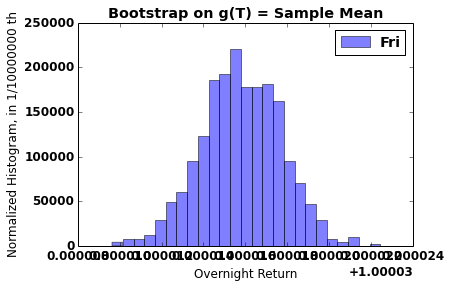
\includegraphics[max size={\textwidth}{\textheight}]{Final_Report_files/Final_Report_100_0.png}
    \par
    \end{center}
    
            \end{InvisibleVerbatim}
            
        
    
\section{Conclusions and Limitations}\label{conclusions-and-limitations}

By now via conventional statistical methods, our group has shown that
Friday evenings over the past decade were not necessarily resulting a
signficiant lower return. However, we acknowledge there are many
aggressive assumptions - and perhaps, loopholes - in our research.

The main difficulty of the research was that we utilized conventional
statistical methods on a time-series finanical data. Oftentimes, as seen
eariler, the methods require each comparison group to possess certain
properties, such as normality, independence among each observations,
IID, and pairwise movements. However, we perhaps shall assume none of
those.

The bootstrapping method was distribution free, meaning that if the data
were correctly accessed, the bootstrap summary yet predicts some
valuable information of the data structure, regardless correlation
within the data set. It is our hope that our audience, at this point,
are somewhat convinced that the Weekend Effect might be just a myth.
        

        \renewcommand{\indexname}{Index}
        \printindex

    % End of document
    \end{document}


